% NIRNAY technical report. Build: latexmk -pdf main.tex (after python gen_data.py).
\documentclass[11pt,a4paper]{article}

% ------------------------------------------------------------------ fonts and page
\usepackage[T1]{fontenc}
\usepackage[utf8]{inputenc}
\usepackage{amsmath}
\usepackage{mathtools}
\usepackage{libertinus}
\usepackage{libertinust1math}
\usepackage[scale=0.93]{sourcesanspro}
\usepackage[scale=0.86]{sourcecodepro}
\usepackage{bm}
\usepackage[a4paper,top=26mm,bottom=28mm,left=26mm,right=26mm,headheight=22pt,headsep=14pt]{geometry}
\usepackage[final]{microtype}
\usepackage{xcolor}
\usepackage{graphicx}

% ------------------------------------------------------------------ branding (from the idea deck)
\definecolor{navy}{HTML}{1F2A44}
\definecolor{saffron}{HTML}{E8702A}
\definecolor{igreen}{HTML}{1E8C45}
\definecolor{ink}{HTML}{2B2F36}
\definecolor{muted}{HTML}{5B6770}
\definecolor{card}{HTML}{F2F4F7}
\definecolor{rule}{HTML}{D5DAE1}
\definecolor{sky}{HTML}{3A6EA5}
\definecolor{plum}{HTML}{8E4585}

% ------------------------------------------------------------------ figures and plots
\usepackage{tikz}
\usetikzlibrary{positioning,arrows.meta,shapes.geometric,shapes.misc,fit,calc,backgrounds,matrix,
  decorations.pathreplacing,patterns}
\usepackage{pgfplots}
\pgfplotsset{compat=1.18}
\usepgfplotslibrary{groupplots,fillbetween}
\usepackage{pgfplotstable}
\usepackage[linguistics]{forest}

% ------------------------------------------------------------------ tables, numbers, boxes, code
\usepackage{booktabs}
\usepackage{tabularx}
\usepackage{longtable}
\usepackage{multirow}
\usepackage{array}
\usepackage[detect-all]{siunitx}
\sisetup{exponent-product=\cdot, retain-zero-exponent=false, group-minimum-digits=5}
\usepackage[most]{tcolorbox}
\usepackage{listings}
\usepackage[ruled,vlined,linesnumbered]{algorithm2e}
\usepackage{enumitem}
\usepackage{caption}
\usepackage{subcaption}
\usepackage[section]{placeins}
\usepackage{titlesec}
\usepackage{fancyhdr}
\usepackage{xurl}
\usepackage[numbers,sort&compress]{natbib}

% hyperref and cleveref last
\usepackage[colorlinks=true,linkcolor=navy,citecolor=igreen,urlcolor=sky,
  pdftitle={NIRNAY: an indigenous LP/MILP/QP solver (SIH26119 technical report)},
  pdfauthor={Team ZeroCloud}]{hyperref}
\usepackage{doi}
\usepackage[capitalise,noabbrev]{cleveref}
\crefname{algocf}{Algorithm}{Algorithms}
\Crefname{algocf}{Algorithm}{Algorithms}

% Layout, colours and drawing styles for the NIRNAY report.

% ------------------------------------------------------------------ headings
\titleformat{\section}{\sffamily\Large\bfseries\color{navy}}{\color{saffron}\thesection}{0.8em}{}
\titleformat{\subsection}{\sffamily\large\bfseries\color{navy}}{\color{saffron}\thesubsection}{0.7em}{}
\titleformat{\subsubsection}{\sffamily\normalsize\bfseries\color{navy}}{\thesubsubsection}{0.6em}{}
\titleformat{\paragraph}[runin]{\sffamily\normalsize\bfseries\color{navy}}{}{0pt}{}[.]
\titlespacing*{\section}{0pt}{3.2ex plus 1ex minus .2ex}{1.6ex plus .2ex}
\titlespacing*{\subsection}{0pt}{2.6ex plus 1ex minus .2ex}{1.1ex plus .2ex}
\titlespacing*{\paragraph}{0pt}{1.4ex plus .5ex minus .2ex}{0.8em}
% sections run on (no \sectionbreak), which keeps floats close to their text

% ------------------------------------------------------------------ header and footer
\pagestyle{fancy}
\fancyhf{}
\renewcommand{\headrulewidth}{0.4pt}
\renewcommand{\headrule}{\hbox to\headwidth{\color{rule}\leaders\hrule height \headrulewidth\hfill}}
\fancyhead[L]{\sffamily\footnotesize\color{muted}NIRNAY \textperiodcentered{} Technical report}
\fancyhead[R]{\sffamily\footnotesize\color{muted}SIH26119 \textperiodcentered{} Team ZeroCloud}
\fancyfoot[C]{\sffamily\footnotesize\color{muted}\thepage}
\fancypagestyle{plain}{\fancyhf{}\renewcommand{\headrulewidth}{0pt}\fancyfoot[C]{\sffamily\footnotesize\color{muted}\thepage}}

% ------------------------------------------------------------------ captions, lists, spacing
\captionsetup{font=small,labelfont={bf,sf,color=navy},format=hang,margin=4pt}
\setlength{\emergencystretch}{3em}
\setlist{itemsep=2pt,topsep=4pt,parsep=0pt}
\setlength{\parindent}{0pt}
\setlength{\parskip}{0.55em plus 0.15em}
\renewcommand{\arraystretch}{1.12}
\setlength{\LTpre}{6pt}
\setlength{\LTpost}{4pt}

% generated table rows: the primitive \input is expandable, so \bottomrule after it still follows a \cr
\makeatletter
\newcommand{\rows}[1]{\@@input #1 }
\makeatother

% ------------------------------------------------------------------ maths shorthands
\newcommand{\R}{\mathbb{R}}
\newcommand{\Z}{\mathbb{Z}}
\newcommand{\T}{^{\mathsf{T}}}
\newcommand{\mT}{^{-\mathsf{T}}}
\newcommand{\diag}{\operatorname{diag}}
\newcommand{\proj}{\operatorname{proj}}
\newcommand{\nnz}{\operatorname{nnz}}
\newcommand{\sign}{\operatorname{sign}}
\newcommand{\fr}{\operatorname{frac}}
\newcommand{\code}[1]{\texttt{#1}}
\newcommand{\file}[1]{\texttt{\small #1}}
\newcommand{\nirnay}{\textsc{Nirnay}}
\DeclareMathOperator{\clip}{clip}

% ------------------------------------------------------------------ boxes
\tcbset{
  nbox/.style={enhanced,colback=card,colframe=navy,boxrule=0.6pt,arc=2pt,left=8pt,right=8pt,top=6pt,bottom=6pt,
    fonttitle=\sffamily\bfseries,coltitle=white,colbacktitle=navy},
  lesson/.style={enhanced,colback=saffron!6,colframe=saffron,boxrule=0.6pt,arc=2pt,left=8pt,right=8pt,top=5pt,bottom=5pt,
    fonttitle=\sffamily\bfseries,coltitle=white,colbacktitle=saffron},
  honest/.style={enhanced,colback=igreen!5,colframe=igreen,boxrule=0.6pt,arc=2pt,left=8pt,right=8pt,top=5pt,bottom=5pt,
    fonttitle=\sffamily\bfseries,coltitle=white,colbacktitle=igreen},
}
\newtcolorbox{keybox}[1][]{nbox,title={#1}}
\newtcolorbox{lessonbox}[1][]{lesson,title={#1}}
\newtcolorbox{honestbox}[1][]{honest,title={#1}}

% a "big number" tile for the at-a-glance panel
\newcommand{\stat}[2]{\begin{minipage}[t]{0.23\linewidth}\centering
  {\sffamily\bfseries\LARGE\color{saffron}#1}\\[1pt]{\sffamily\scriptsize\color{ink}#2}\end{minipage}}

% ------------------------------------------------------------------ listings
\lstset{basicstyle=\ttfamily\small,columns=fullflexible,keepspaces=true,
  keywordstyle=\color{navy}\bfseries,commentstyle=\color{muted}\itshape,stringstyle=\color{igreen},
  frame=single,rulecolor=\color{rule},backgroundcolor=\color{card},xleftmargin=6pt,xrightmargin=6pt,
  framesep=4pt,breaklines=true,showstringspaces=false}

% ------------------------------------------------------------------ algorithm2e
\SetAlgoSkip{medskip}
\SetKwComment{Comment}{\color{muted}$\triangleright$\ }{}
\SetCommentSty{textit}
\SetKwInOut{Input}{input}
\SetKwInOut{Output}{output}
\SetAlFnt{\small}
\SetAlCapFnt{\small\sffamily\bfseries}
\SetAlCapNameFnt{\small}
\renewcommand{\listalgorithmcfname}{List of Algorithms}

% ------------------------------------------------------------------ TikZ styles
\tikzset{
  >={Stealth[length=2.2mm]},
  blk/.style={draw=navy,fill=white,rounded corners=2pt,line width=0.6pt,align=center,
    font=\sffamily\footnotesize,minimum height=7mm,inner sep=3pt},
  blkn/.style={blk,fill=navy,text=white},
  blks/.style={blk,draw=saffron,fill=saffron!10},
  blkg/.style={blk,draw=igreen,fill=igreen!8},
  blkm/.style={blk,draw=muted,fill=card},
  dec/.style={diamond,aspect=2.1,draw=saffron,fill=saffron!10,line width=0.6pt,align=center,
    font=\sffamily\scriptsize,inner sep=1pt},
  term/.style={rounded rectangle,draw=navy,fill=navy,text=white,font=\sffamily\footnotesize\bfseries,
    minimum height=6.5mm,inner xsep=6pt},
  flow/.style={->,draw=ink,line width=0.6pt},
  lbl/.style={font=\sffamily\scriptsize,color=muted},
  layer/.style={draw=rule,fill=card,rounded corners=3pt,line width=0.5pt},
}

% ------------------------------------------------------------------ PGFPlots styles
\pgfplotsset{
  every axis/.append style={font=\sffamily\footnotesize, tick label style={font=\sffamily\scriptsize},
    label style={font=\sffamily\footnotesize}, legend style={font=\sffamily\scriptsize,draw=rule,fill=white,fill opacity=0.9,text opacity=1},
    axis line style={draw=muted}, tick style={draw=muted}, major grid style={draw=rule,line width=0.3pt},
    minor grid style={draw=rule!50,line width=0.2pt}},
  nspx/.style={color=saffron,line width=1.1pt},
  nipm/.style={color=sky,line width=1.1pt},
  nhighs/.style={color=navy,line width=1.1pt,dashed},
  nbest/.style={color=igreen,line width=1.1pt,dotted},
  npdlp/.style={color=plum,line width=1.1pt},
}

% generated by gen_data.py; do not edit
\newcommand{\CompLpInstances}{\texttt{25fv47}, \texttt{adlittle}, \texttt{afiro}, \texttt{blend}, \texttt{degen2}, \texttt{ex10}, \texttt{greenbea}, \texttt{pilot4}, \texttt{qap15}, \texttt{sc50a}, \texttt{share2b}, \texttt{stocfor1}}
\newcommand{\CompMipInstances}{\texttt{bell5}, \texttt{egout}, \texttt{flugpl}, \texttt{lseu}, \texttt{misc03}, \texttt{mod008}, \texttt{p0033}, \texttt{p0201}, \texttt{p0282}, \texttt{stein27}}
\newcommand{\CompQpInstances}{\texttt{CVXQP1\_S}, \texttt{DUALC1}, \texttt{HS21}, \texttt{HS35}, \texttt{PRIMALC1}, \texttt{QADLITTL}, \texttt{QAFIRO}, \texttt{QPCBLEND}, \texttt{QSC205}, \texttt{QSHARE2B}}
\newcommand{\barCount}{5}
\newcommand{\barLabels}{Netlib/simplex,Netlib/IPM,Netlib/PDLP,MIPLIB3/BnB,Maros/QP-IPM}
\newcommand{\bestOfTwoRatio}{2.2}
\newcommand{\censusColsPct}{4.8}
\newcommand{\censusMaxRowsName}{ship12s}
\newcommand{\censusMaxRowsPct}{60}
\newcommand{\censusMaxTime}{3.65}
\newcommand{\censusMaxTimeName}{dfl001}
\newcommand{\censusMedRowsPct}{7.7}
\newcommand{\censusNnzPct}{7.6}
\newcommand{\censusRowsPct}{10.5}
\newcommand{\censusSolved}{0}
\newcommand{\censusTime}{43.9}
\newcommand{\censusUntouched}{16}
\newcommand{\dualBadNames}{none}
\newcommand{\dualMaxY}{\num{2.5e-13}}
\newcommand{\dualMaxZ}{\num{2.0e-12}}
\newcommand{\dualStatusNames}{\texttt{dfl001} (time\_limit), \texttt{pilot87} (time\_limit)}
\newcommand{\fasterMipNames}{\texttt{air03}, \texttt{nw04}}
\newcommand{\fasterMipVoneNames}{\texttt{air03}}
\newcommand{\flTime}{592}
\newcommand{\genDate}{2026-09-30}
\newcommand{\gmrIpm}{3.4}
\newcommand{\gmrSpx}{6.8}
\newcommand{\haveCaseRuns}{1}
\newcommand{\haveCensus}{1}
\newcommand{\haveCompLp}{1}
\newcommand{\haveCompMip}{1}
\newcommand{\haveCompQp}{1}
\newcommand{\haveDualCheck}{1}
\newcommand{\haveInProgress}{0}
\newcommand{\haveIpm}{1}
\newcommand{\haveIpmNew}{0}
\newcommand{\haveLarge}{1}
\newcommand{\haveMip}{1}
\newcommand{\haveMipNew}{0}
\newcommand{\haveMipVtwo}{1}
\newcommand{\havePdlp}{1}
\newcommand{\havePdlpNew}{0}
\newcommand{\haveQp}{1}
\newcommand{\haveQpNew}{0}
\newcommand{\haveQpVone}{1}
\newcommand{\haveSpx}{1}
\newcommand{\haveSpxNew}{0}
\newcommand{\haveSpxPresolve}{1}
\newcommand{\inProgressList}{none}
\newcommand{\ipmComplete}{1}
\newcommand{\ipmFailNames}{\texttt{dfl001}, \texttt{greenbea}, \texttt{pilot}, \texttt{pilot87}}
\newcommand{\ipmFile}{netlib\_ipm\_v2.csv}
\newcommand{\ipmVer}{v2}
\newcommand{\ipmVerNum}{2}
\newcommand{\largeCpuHw}{Intel64 Family 6 Model 141 Stepping 1}
\newcommand{\largeGpuHw}{NVIDIA GeForce RTX 3050 Laptop GPU}
\newcommand{\largeGpuOnlyNames}{\texttt{rail02}, \texttt{s250r10}, \texttt{square41}}
\newcommand{\largeLimit}{300}
\newcommand{\largeNames}{datt256,ex10,neos-5052403-cygnet,qap15,rail01,rail02,rmine15,s100,s250r10,savsched1,square41}
\newcommand{\largeSpeedGm}{2.5}
\newcommand{\largeSpeedMax}{5.8}
\newcommand{\largeSpeedMin}{1.2}
\newcommand{\largeTol}{$10^{-4}$}
\newcommand{\largeVsHighsMax}{321}
\newcommand{\largeVsHighsMin}{0.3}
\newcommand{\locAll}{7416}
\newcommand{\locBench}{1316}
\newcommand{\locCases}{1938}
\newcommand{\locCore}{5063}
\newcommand{\locTests}{548}
\newcommand{\maxErrIpm}{7.2e-07}
\newcommand{\maxErrPdlp}{5.1e-02}
\newcommand{\maxErrSpx}{5.5e-09}
\newcommand{\maxItIpm}{67}
\newcommand{\maxItPdlp}{529152}
\newcommand{\maxItQp}{78}
\newcommand{\maxItSpx}{22000}
\newcommand{\maxNodesMip}{112067}
\newcommand{\maxNodesMipVone}{53129}
\newcommand{\maxrIpm}{159}
\newcommand{\maxrSpx}{26}
\newcommand{\maxtIpm}{184.5}
\newcommand{\maxtNameIpm}{fit2p}
\newcommand{\maxtNameSpx}{dfl001}
\newcommand{\maxtSpx}{22.7}
\newcommand{\medErrIpm}{9.0e-11}
\newcommand{\medErrPdlp}{3.4e-05}
\newcommand{\medErrQp}{1.7e-10}
\newcommand{\medErrSpx}{3.6e-16}
\newcommand{\medItIpm}{20}
\newcommand{\medItPdlp}{7392}
\newcommand{\medItQp}{14}
\newcommand{\medItSpx}{440}
\newcommand{\medNodesMip}{648}
\newcommand{\medNodesMipVone}{445}
\newcommand{\medrIpm}{2.8}
\newcommand{\medrSpx}{6.7}
\newcommand{\mipComplete}{1}
\newcommand{\mipFile}{miplib3\_bnb\_v2.csv}
\newcommand{\mipFoundNotProvedNames}{\texttt{bell3a}, \texttt{danoint}, \texttt{misc07}, \texttt{noswot}, \texttt{stein45}}
\newcommand{\mipGainedNames}{\texttt{bell5}, \texttt{fiber}, \texttt{gesa2\_o}, \texttt{mitre}, \texttt{mod008}, \texttt{nw04}, \texttt{p2756}, \texttt{qnet1}, \texttt{rentacar}}
\newcommand{\mipLostNames}{\texttt{gt2}}
\newcommand{\mipLpItersPerNode}{34}
\newcommand{\mipNewerDone}{64}
\newcommand{\mipNewerFile}{miplib3\_bnb\_v2.csv}
\newcommand{\mipNewerPartial}{0}
\newcommand{\mipNewerSolved}{33}
\newcommand{\mipNoIncumbentNames}{\texttt{10teams}, \texttt{air04}, \texttt{air05}, \texttt{dano3mip}, \texttt{fast0507}, \texttt{mkc}, \texttt{seymour}, \texttt{swath}}
\newcommand{\mipNodesPerSec}{141}
\newcommand{\mipOnlyUsNames}{\texttt{nw04}}
\newcommand{\mipOtherStatusNames}{none}
\newcommand{\mipVer}{v2}
\newcommand{\mipVerNum}{2}
\newcommand{\nBothSolved}{86}
\newcommand{\nCaseRuns}{7}
\newcommand{\nCaseRunsOptimal}{5}
\newcommand{\nCases}{7}
\newcommand{\nCensus}{90}
\newcommand{\nCompLpInst}{12}
\newcommand{\nCompLpSolvers}{20}
\newcommand{\nCompMipInst}{10}
\newcommand{\nCompMipSolvers}{9}
\newcommand{\nCompQpInst}{10}
\newcommand{\nCompQpSolvers}{5}
\newcommand{\nDualBad}{0}
\newcommand{\nDualOk}{88}
\newcommand{\nDualStatus}{2}
\newcommand{\nDualTot}{90}
\newcommand{\nFasterIpm}{6}
\newcommand{\nFasterMip}{2}
\newcommand{\nFasterMipVone}{1}
\newcommand{\nFasterQp}{9}
\newcommand{\nFasterSpx}{0}
\newcommand{\nFixedIpm}{6}
\newcommand{\nFixedIpmSpeedup}{8.8}
\newcommand{\nFixedIpmVOne}{80}
\newcommand{\nFixedIpmVOneRatio}{31.3}
\newcommand{\nFixedIpmVOneSgm}{1.37}
\newcommand{\nFixedIpmVOneTot}{90}
\newcommand{\nFixedSpx}{6}
\newcommand{\nFixedSpxSpeedup}{1.2}
\newcommand{\nFixedSpxVOne}{84}
\newcommand{\nFixedSpxVOneRatio}{4.6}
\newcommand{\nFixedSpxVOneSgm}{0.46}
\newcommand{\nFixedSpxVOneTot}{90}
\newcommand{\nIpm}{86}
\newcommand{\nIpmFasterThanSpx}{66}
\newcommand{\nIpmNear}{3}
\newcommand{\nIpmTot}{90}
\newcommand{\nLarge}{11}
\newcommand{\nLargeBothOk}{7}
\newcommand{\nLargeGpuOnly}{3}
\newcommand{\nLargeList}{11}
\newcommand{\nLargeNeither}{1}
\newcommand{\nMarosFiles}{138}
\newcommand{\nMip}{33}
\newcommand{\nMipBothOpt}{32}
\newcommand{\nMipCommon}{64}
\newcommand{\nMipCutsGained}{9}
\newcommand{\nMipCutsLost}{1}
\newcommand{\nMipFoundNotProved}{5}
\newcommand{\nMipGapBelowOnePct}{6}
\newcommand{\nMipGapBelowTenPct}{15}
\newcommand{\nMipIncumbent}{23}
\newcommand{\nMipList}{64}
\newcommand{\nMipNoIncumbent}{8}
\newcommand{\nMipOnlyUs}{1}
\newcommand{\nMipOtherStatus}{0}
\newcommand{\nMipRefOnly}{15}
\newcommand{\nMipRefOpt}{47}
\newcommand{\nMipRefTL}{17}
\newcommand{\nMipSmallInt}{23}
\newcommand{\nMipTot}{64}
\newcommand{\nMipVone}{25}
\newcommand{\nMipVoneFoundNotProved}{3}
\newcommand{\nMipVoneGapBelowOnePct}{3}
\newcommand{\nMipVoneGapBelowTenPct}{13}
\newcommand{\nMipVoneIncumbent}{26}
\newcommand{\nMipVoneNoIncumbent}{12}
\newcommand{\nMipVoneRefOpt}{45}
\newcommand{\nMipVoneRefTL}{19}
\newcommand{\nMipVoneSmallInt}{23}
\newcommand{\nMipVoneTot}{64}
\newcommand{\nMipVoneWrongOpt}{0}
\newcommand{\nMipWrongOpt}{0}
\newcommand{\nMiplibFiles}{64}
\newcommand{\nNetlibFiles}{90}
\newcommand{\nPdlp}{86}
\newcommand{\nPdlpIterLimit}{4}
\newcommand{\nPdlpLoose}{78}
\newcommand{\nPdlpStrict}{15}
\newcommand{\nPdlpTight}{59}
\newcommand{\nPdlpTimeLimit}{0}
\newcommand{\nPdlpTot}{90}
\newcommand{\nPresolveCommon}{90}
\newcommand{\nPresolveFail}{0}
\newcommand{\nProf}{90}
\newcommand{\nQp}{121}
\newcommand{\nQpAlmostRef}{9}
\newcommand{\nQpFail}{16}
\newcommand{\nQpList}{138}
\newcommand{\nQpLoose}{0}
\newcommand{\nQpLooseOrWrong}{0}
\newcommand{\nQpNumErr}{12}
\newcommand{\nQpOptimalStatus}{121}
\newcommand{\nQpOther}{4}
\newcommand{\nQpRefAnnotated}{4}
\newcommand{\nQpRefBad}{1}
\newcommand{\nQpRefFail}{1}
\newcommand{\nQpTot}{138}
\newcommand{\nQpVone}{111}
\newcommand{\nQpVoneTot}{138}
\newcommand{\nQpWrong}{0}
\newcommand{\nQpWrongBig}{0}
\newcommand{\nSpx}{90}
\newcommand{\nSpxTot}{90}
\newcommand{\nSpxVtwo}{90}
\newcommand{\nTestFunctions}{31}
\newcommand{\netlibMaxCols}{13525}
\newcommand{\netlibMaxName}{maros-r7}
\newcommand{\netlibMaxNnz}{144848}
\newcommand{\netlibMaxRows}{6071}
\newcommand{\netlibMinRows}{24}
\newcommand{\netlibTotNnz}{1093989}
\newcommand{\pdlpComplete}{1}
\newcommand{\pdlpFile}{netlib\_pdlp.csv}
\newcommand{\pdlpIterLimitNames}{\texttt{bnl1}, \texttt{greenbea}, \texttt{perold}, \texttt{pilot4}}
\newcommand{\pdlpTimeLimitNames}{none}
\newcommand{\pdlpVer}{v1}
\newcommand{\pdlpVerNum}{1}
\newcommand{\pdlpWorst}{\texttt{forplan} (\num{5.1e-02}), \texttt{ganges} (\num{1.8e-02}), \texttt{bnl2} (\num{5.6e-03}), \texttt{finnis} (\num{3.9e-03}), \texttt{scrs8} (\num{3.3e-03}), \texttt{pilot} (\num{1.7e-03})}
\newcommand{\presolveDone}{90}
\newcommand{\presolveFailNames}{none}
\newcommand{\presolveFaster}{1}
\newcommand{\presolveFile}{netlib\_simplex\_v4.csv}
\newcommand{\presolveGmrHighs}{6.8}
\newcommand{\presolveGmrHighsCommon}{6.8}
\newcommand{\presolveGmrHighsCommonVtwo}{6.3}
\newcommand{\presolveIterRatio}{1.13}
\newcommand{\presolveLoad}{0.8}
\newcommand{\presolvePartial}{0}
\newcommand{\presolveRatioHighs}{3.1}
\newcommand{\presolveRatioHighsVtwo}{3.7}
\newcommand{\presolveSmallWorse}{1}
\newcommand{\presolveSolved}{90}
\newcommand{\presolveSpeedup}{1.49}
\newcommand{\profTauMax}{238}
\newcommand{\qpAlmostRefNames}{\texttt{LISWET1}, \texttt{LISWET10}, \texttt{LISWET11}, \texttt{LISWET12}, \texttt{LISWET7}, \texttt{LISWET8}, \texttt{LISWET9}, \texttt{UBH1}, \texttt{YAO}}
\newcommand{\qpComplete}{1}
\newcommand{\qpFile}{maros\_qpipm\_v2.csv}
\newcommand{\qpLooseNames}{none}
\newcommand{\qpMaxN}{93263}
\newcommand{\qpMaxNName}{BOYD2}
\newcommand{\qpNumErrNames}{\texttt{HUES-MOD}, \texttt{HUESTIS}, \texttt{KSIP}, \texttt{LISWET1}, \texttt{LISWET10}, \texttt{LISWET11}, \texttt{LISWET12}, \texttt{LISWET7}, \texttt{LISWET8}, \texttt{LISWET9}, \texttt{UBH1}, \texttt{YAO}}
\newcommand{\qpOtherNames}{\texttt{CONT-300}, \texttt{CVXQP1\_L}, \texttt{CVXQP2\_L}, \texttt{CVXQP3\_L}}
\newcommand{\qpRefBadNames}{\texttt{BOYD2}}
\newcommand{\qpRefFailNames}{\texttt{BOYD2}}
\newcommand{\qpVer}{v2}
\newcommand{\qpVerNum}{2}
\newcommand{\qpWrongBigNames}{none}
\newcommand{\ratioIpm}{3.3}
\newcommand{\ratioIpmTenShift}{7.2}
\newcommand{\ratioMip}{4.4}
\newcommand{\ratioMipVone}{9.1}
\newcommand{\ratioPdlp}{4.6}
\newcommand{\ratioQp}{1.4}
\newcommand{\ratioSpx}{3.1}
\newcommand{\ratioSpxTenShift}{3.9}
\newcommand{\rhoOneHighs}{0.93}
\newcommand{\rhoOneIpm}{0.07}
\newcommand{\rhoOneSpx}{0.00}
\newcommand{\rhoTenIpm}{0.82}
\newcommand{\rhoTenSpx}{0.67}
\newcommand{\sgmIpm}{0.23}
\newcommand{\sgmIpmRef}{0.070}
\newcommand{\sgmMip}{6.67}
\newcommand{\sgmMipRef}{1.50}
\newcommand{\sgmMipVone}{10.91}
\newcommand{\sgmMipVoneRef}{1.19}
\newcommand{\sgmPdlp}{0.43}
\newcommand{\sgmPdlpRef}{0.094}
\newcommand{\sgmQp}{0.43}
\newcommand{\sgmQpRef}{0.30}
\newcommand{\sgmSpx}{0.28}
\newcommand{\sgmSpxRef}{0.090}
\newcommand{\shiftA}{1}
\newcommand{\shiftB}{10}
\newcommand{\spxComplete}{1}
\newcommand{\spxFile}{netlib\_simplex\_v4.csv}
\newcommand{\spxHasPresolve}{1}
\newcommand{\spxVer}{v4}
\newcommand{\spxVerNum}{4}
\newcommand{\sweepLoadRatio}{0.7}
\newcommand{\tauAllIpm}{159}
\newcommand{\tauAllSpx}{26}
\newcommand{\tlMip}{60}
\newcommand{\tlNetlib}{300}
\newcommand{\tlPdlp}{120}
\newcommand{\tlQp}{120}
\newcommand{\totIpm}{208}
\newcommand{\totRefIpm}{7.3}
\newcommand{\totRefSpx}{13.9}
\newcommand{\totSpx}{68}
\newcommand{\ucGap}{0.73}
\newcommand{\ucGapTarget}{1}
\newcommand{\verClarabel}{0.11.1}
\newcommand{\verCupy}{14.2.0}
\newcommand{\verHighs}{1.15.1}
\newcommand{\verNumba}{0.65.0}
\newcommand{\verNumpy}{2.4.6}
\newcommand{\verPython}{3.12.10}


\begin{document}

\pagenumbering{Alph}
% Title page with the SIH26119 identifiers.
\begin{titlepage}
\thispagestyle{empty}
\begin{tikzpicture}[remember picture,overlay]
  \fill[navy] (current page.north west) rectangle ([yshift=-88mm]current page.north east);
  \fill[saffron] ([yshift=-88mm]current page.north west) rectangle ([yshift=-91mm]current page.north east);
  \fill[igreen] ([yshift=-91mm]current page.north west) rectangle ([yshift=-92.5mm]current page.north east);
  % a small sparse-matrix motif in the band
  \begin{scope}[shift={([xshift=-62mm,yshift=-18mm]current page.north east)}]
    \foreach \i/\j in {0/0,1/1,2/2,3/3,4/4,5/5,6/6,0/3,3/0,1/5,5/1,2/6,6/2,4/6,6/4,0/6,6/0,3/5,5/3}{
      \fill[white,opacity=0.85] (\j*6mm,-\i*6mm) rectangle ++(4.6mm,-4.6mm);}
    \foreach \i/\j in {1/3,3/1,2/5,5/2}{\fill[saffron] (\j*6mm,-\i*6mm) rectangle ++(4.6mm,-4.6mm);}
  \end{scope}
  \node[anchor=north west,text=white,font=\sffamily\bfseries\small,align=left]
    at ([xshift=26mm,yshift=-18mm]current page.north west) {SMART INDIA HACKATHON 2026\\[1pt]
    \mdseries Problem statement SIH26119};
  \node[anchor=north west,text=white,font=\sffamily\bfseries,align=left]
    at ([xshift=25mm,yshift=-36mm]current page.north west) {\fontsize{46}{50}\selectfont NIRNAY};
  \node[anchor=north west,text=white,font=\sffamily\large,align=left,text width=105mm]
    at ([xshift=26mm,yshift=-58mm]current page.north west)
    {An indigenous LP\,/\,MILP\,/\,QP optimisation solver, written from the mathematics up};
\end{tikzpicture}

\vspace*{92mm}

{\sffamily\LARGE\bfseries\color{navy} Technical report}\par\vspace{2mm}
{\sffamily\large\color{muted} Algorithms, numerical safeguards, verification and benchmark results}\par
\vspace{14mm}

\renewcommand{\arraystretch}{1.45}
{\sffamily\small
\begin{tabularx}{\linewidth}{@{}>{\bfseries\color{navy}}l@{\hspace{8mm}}X@{}}
Problem statement ID & SIH26119\\
Problem statement title & Indigenous GPU-Accelerated Optimization Solver (Sovereign Alternative to \mbox{Xpress/CPLEX})\\
Organisation & Mangalore Refinery and Petrochemicals Limited (MRPL)\\
Theme & Smart Automation\\
Category & Software\\
Team & ZeroCloud\\
Software & \nirnay{} 0.1.0 (Python~\verPython, NumPy~\verNumpy, Numba~\verNumba, CuPy~\verCupy)\\
Date & \today\\
\end{tabularx}}

\vfill
{\sffamily\footnotesize\color{muted}
Every benchmark number in this report is read from the CSV files in \file{results/} by
\file{deliverables/report/gen\_data.py}; none is typed by hand. Rebuilding after a new sweep updates the
text, tables and plots together.}
\end{titlepage}


\pagenumbering{roman}
% Abstract and the at-a-glance panel.
\section*{Summary}
\addcontentsline{toc}{section}{Summary}

Problem statement SIH26119 asks for an optimisation solver that India owns: one that reads the
models refinery planners already write, solves linear, mixed-integer and quadratic programmes,
uses GPUs where they help, and is not built on Xpress, CPLEX or any other existing solver library.
\nirnay{} is our answer. Every algorithm and every factorisation in it is implemented in the
repository: an MPS/QPS reader, presolve with exact primal and dual postsolve, scaling, a
Gilbert--Peierls sparse LU with eta updates and basis repair, an up-looking sparse Cholesky, a
quasi-definite $LDL\T$, a minimum-degree ordering, a bounded dual simplex, a Mehrotra
interior-point method, a restarted primal--dual hybrid gradient method (PDLP) on CPU and GPU, a
branch-and-bound code with reliability branching, propagation, heuristics and Gomory cuts, and a
QP interior-point method. HiGHS and Clarabel appear only in the benchmark harness, as independent
references that check every answer.

This report describes each algorithm as the code implements it, with its equations and
pseudocode; the numerical failures we hit and how each fix works; how answers are verified; and
the benchmark results, failures included. \Cref{sec:results} states plainly where \nirnay{} is behind:
it is slower than HiGHS, and it proves fewer MIPLIB instances optimal.

\begin{keybox}[At a glance (generated from \file{results/})]
\centering
\stat{\nSpx/\nSpxTot}{Netlib LPs solved by the dual simplex (objective within $10^{-6}$ of HiGHS)}\hfill
\stat{\nIpm/\nIpmTot}{Netlib LPs solved by the interior-point method}\hfill
\stat{\nQp/\nQpTot}{Maros--Mészáros convex QPs solved (within $10^{-6}$ of Clarabel)}\hfill
\stat{\nMip/\nMipTot}{MIPLIB\,3 instances proven optimal in \tlMip\,s\ifnum\nMipTot<\nMipList{} (sweep in progress)\fi}
\par\medskip
\stat{\ratioSpx$\times$}{dual simplex time vs.\ HiGHS, shifted geometric mean (shift \shiftA\,s)}\hfill
\stat{\gmrSpx$\times$}{dual simplex vs.\ HiGHS, geometric mean of per-instance ratios}\hfill
\stat{\largeSpeedMax$\times$}{largest GPU-over-CPU speed-up of our PDLP on the large LPs\ifnum\nLarge<\nLargeList{} run so far\fi}\hfill
\stat{\nDualBad}{dual-feasibility failures in \nDualOk{} Netlib solutions checked after postsolve}
\end{keybox}

\begin{honestbox}[Where we stand]
\nirnay{} is correct on the standard LP and QP test sets and substantially slower than a mature
open-source solver: the dual simplex takes \ratioSpx{} times as long as HiGHS in shifted geometric
mean over the \nSpxTot{} Netlib problems (\ratioSpxTenShift{} times with a \shiftB\,s shift, and
\gmrSpx{} times as the geometric mean of per-instance ratios). On MIPLIB\,3 with a \tlMip\,s limit,
branch-and-bound proves \nMip{} of the \nMipTot{} instances\ifnum\nMipTot<\nMipList{} run so far\fi{} optimal, against
\nMipRefOpt{} for HiGHS under the same limit. The engines are compiled with Numba inside the
inner loops, but the iteration drivers are Python, and the MIP code lacks most of the presolve,
cut families and heuristics that close gaps in production solvers.
\end{honestbox}

\clearpage
\tableofcontents
\clearpage
\listoffigures
\listoftables
\listofalgorithms
\clearpage
\pagenumbering{arabic}

% Section 1: problem statement and motivation.
\section{Problem statement and motivation}\label{sec:intro}

\subsection{The problem statement}
MRPL's problem statement SIH26119, \emph{Indigenous GPU-Accelerated Optimization Solver (Sovereign
Alternative to Xpress/CPLEX)}, starts from a practical dependency. Refinery crude selection,
blending, production planning, scheduling and product distribution in India are formulated as
linear and mixed-integer programmes and solved with a small number of foreign commercial solvers.
Those solvers are closed: their licences cost money every year, their algorithms cannot be
inspected or adapted, and their availability depends on vendors outside the country. The
statement asks for a solver that is developed here, handles the same problem classes, can use
GPUs, and does not build on any existing solver library.

We read four requirements out of it:
\begin{enumerate}[label=\textbf{R\arabic*}]
  \item \textbf{Problem classes:} linear programmes (LP), mixed-integer linear programmes (MILP)
        and convex quadratic programmes (QP), the classes that planning and scheduling models
        fall into.
  \item \textbf{Independence:} no dependence on an existing optimisation solver or sparse direct
        solver library. The factorisations, orderings and algorithms must be our own code.
  \item \textbf{Interoperability:} read the MPS and QPS files that modelling tools and every
        public benchmark library already produce.
  \item \textbf{Acceleration:} use a GPU where the algorithm can exploit one.
\end{enumerate}

\subsection{What \nirnay{} is}
\nirnay{} (Sanskrit/Hindi \emph{nirṇay}, ``decision'') is a Python package whose compute
kernels are compiled to machine code with Numba and, for the GPU path, to CUDA with CuPy. It has
three LP engines, which suit different problem shapes:
\begin{itemize}
  \item a \textbf{bounded dual simplex} (\cref{sec:simplex}), which produces vertex solutions and
        re-solves quickly after a bound change: this is the engine branch-and-bound uses;
  \item a \textbf{primal--dual interior-point method} (\cref{sec:ipm}), whose iteration count
        grows only slowly with problem size;
  \item \textbf{PDLP}, a restarted primal--dual hybrid gradient method (\cref{sec:pdlp}). It needs
        only products with $A$ and $A\T$, so it runs on a GPU and scales to LPs too large to
        factorise.
\end{itemize}
On top of these sit a \textbf{branch-and-bound} MILP solver (\cref{sec:mip}) and a \textbf{QP
interior-point} method (\cref{sec:qp}). \Cref{fig:arch} shows how the parts fit together.

\subsection{Design principles}
\begin{description}[style=nextline,leftmargin=1.2em,font=\sffamily\bfseries\color{navy}]
  \item[Implement, do not wrap.] Every factorisation (LU, Cholesky, $LDL\T$), ordering and
        solver loop is in the repository. The code depends on NumPy arrays and the Numba
        compiler, plus CuPy for the GPU path. It depends on no optimisation or sparse-direct
        library. \Cref{tab:modules} lists the modules with their sizes.
  \item[Follow the primary literature.] Each module's docstring cites the papers its algorithm
        comes from, and this report follows those citations. Where the code departs from a
        paper, the report says so.
  \item[Verify every answer independently.] Benchmarks run every instance in its own process
        and re-solve it with a reference solver (HiGHS for LP and MILP, Clarabel for QP) that
        reads the file with its own parser (\cref{sec:verification}).
  \item[Report failures.] Tables in this report list every instance, solved or not, and
        \cref{sec:results} analyses the failures.
\end{description}

\subsection{Contributions and outline}
\Cref{sec:formulation} fixes the mathematical forms. \Cref{sec:architecture} describes the system
and the path of a solve, and \cref{sec:presolve} the presolve and postsolve. \Cref{sec:linalg}
covers the sparse linear algebra on which every engine rests. \Cref{sec:simplex,sec:ipm,sec:pdlp}
describe the three LP engines, \cref{sec:mip} branch-and-bound and \cref{sec:qp} the QP method.
\Cref{sec:safeguards} collects the numerical failures we met and how each was fixed.
\Cref{sec:verification} explains how answers are checked, \cref{sec:results} gives the benchmark
results, \cref{sec:cases} the industrial case studies built from Indian public data,
\cref{sec:competitors} a hands-on comparison with other solvers, and \cref{sec:roadmap} the
limitations and next steps. The appendices list every benchmark instance and the typesetting
toolchain of this report.

% Section 2: mathematical formulations.
\section{Mathematical formulations}\label{sec:formulation}

\subsection{The model every engine reads}
All engines read one problem form (\file{nirnay/model.py}):
\begin{equation}\label{eq:model}
\begin{aligned}
  \min_{x\in\R^n}\quad & c\T x + \tfrac12 x\T Q x + c_0\\
  \text{s.t.}\quad & r^{l} \le A x \le r^{u},\\
  & \ell \le x \le u,\\
  & x_j\in\Z \quad (j\in\mathcal{I}),
\end{aligned}
\end{equation}
with $A\in\R^{m\times n}$ sparse, $Q\in\R^{n\times n}$ symmetric positive semidefinite (absent for
LP and MILP), and bounds that may be infinite. A row with $r^l_i=r^u_i$ is an equality, a row with
both bounds finite and different is a ranged row, and a row with neither bound is free. A
maximisation is stored negated with a flag \code{sense}$=-1$, so every engine minimises and the
reported objective and duals come back in the sense of the file. The problem is an LP when
$Q=0$ and $\mathcal{I}=\emptyset$, a MILP when $\mathcal{I}\ne\emptyset$, and a QP when $Q\ne0$.

$A$ is held in compressed sparse column (CSC) form: \code{colptr} (length $n+1$), \code{rowidx}
and \code{vals} (length $\nnz(A)$). The simplex, the LU factorisation and presolve all traverse
columns. Row access, which propagation and the pivot row need, uses $A\T$ in CSC form (that is,
$A$ in CSR form), built once and cached. The arrays are plain NumPy arrays so that Numba kernels
can take them directly.

\subsection{Duality and optimality conditions}
For the LP case ($Q=0$) of \eqref{eq:model}, let $y\in\R^m$ be the row duals and
$z = c - A\T y$ the reduced costs. A primal feasible $x$ is optimal if and only if there is a $y$
with
\begin{equation}\label{eq:kkt-lp}
\begin{aligned}
  y_i > 0 &\Rightarrow a_i\T x = r^l_i, & y_i < 0 &\Rightarrow a_i\T x = r^u_i,\\
  z_j > 0 &\Rightarrow x_j = \ell_j,    & z_j < 0 &\Rightarrow x_j = u_j .
\end{aligned}
\end{equation}
The dual objective is
\begin{equation}\label{eq:dualobj}
  \phi(y) = \sum_i \bigl( r^l_i\, y_i^+ - r^u_i\, y_i^- \bigr)
          + \sum_j \bigl( \ell_j\, z_j^+ - u_j\, z_j^- \bigr) + c_0,
  \qquad t^+=\max(t,0),\; t^-=\max(-t,0),
\end{equation}
and weak duality $c\T x + c_0 \ge \phi(y)$ holds for every primal feasible $x$ and every $y$ for
which \eqref{eq:dualobj} is finite. \Cref{sec:verification} tests \eqref{eq:kkt-lp} on the
solutions \nirnay{} returns, after postsolve and in the original, unscaled variables.

For QP the reduced cost becomes $z = c + Qx - A\T y$ and the dual objective gains the term
$-\tfrac12 x\T Q x$.

\subsection{Computational forms}
Each engine converts \eqref{eq:model} into the form its algebra needs. Each conversion is exact,
and each engine maps its solution back itself.

\paragraph{Simplex: logicals for every row}
The dual simplex (\cref{sec:simplex}) gives every row a logical variable $s_i = a_i\T x$:
\begin{equation}\label{eq:simplex-form}
  \min\; c\T x \quad \text{s.t.}\quad A x - s = 0,\qquad \ell\le x\le u,\qquad r^l\le s\le r^u .
\end{equation}
There are $n+m$ variables and every constraint is an equality with right-hand side zero. The
constraint matrix is $[A\;\; {-I}]$, so the all-logical basis $B=-I$ is always available and
needs no factorisation. Each variable has one of five statuses: basic, at its lower bound, at its
upper bound, nonbasic free at zero, or fixed.

\paragraph{Interior point: bounded standard form}
The IPM (\cref{sec:ipm}) keeps equality rows as they are. It gives every inequality row a slack
column ($a_i\T x - s_i = 0$, $r^l_i\le s_i\le r^u_i$), drops free rows, and substitutes fixed
columns into the right-hand side. It then shifts every variable, and reflects the ones with only
an upper bound, so that each variable is free, nonnegative, or in a box $[0,U_j]$:
\begin{equation}\label{eq:ipm-form}
  \min\; c\T x\quad\text{s.t.}\quad Bx = b,\qquad x_j\ge0\ (j\in\mathcal{L}),\qquad
  x_j + w_j = U_j,\ w_j\ge0\ (j\in\mathcal{U}),
\end{equation}
where $\mathcal{U}\subseteq\mathcal{L}$ are the boxed variables and the rest are free. This is the
bounded standard form of Lustig, Marsten and Shanno~\cite{lustig1994}. The dual has $y$ for the
rows, $z\ge0$ on $x_{\mathcal{L}}\ge0$ and $s\ge0$ on $w\ge0$, and the optimality conditions are
\begin{equation}\label{eq:ipm-kkt}
  Bx=b,\quad x_{\mathcal U}+w=U,\quad B\T y + z - s = c,\quad
  x_j z_j = 0\ (j\in\mathcal L),\quad w_j s_j = 0\ (j\in\mathcal U).
\end{equation}

\paragraph{PDLP: the saddle point on the original rows}
PDLP (\cref{sec:pdlp}) uses the original rows and bounds, with no slack columns, and solves the
saddle-point problem
\begin{equation}\label{eq:saddle}
  \min_{x\in X}\;\max_{y\in Y}\; \mathcal{L}(x,y)= c\T x - y\T A x + p(y),\qquad
  p(y) = (r^l)\T y^+ - (r^u)\T y^-,
\end{equation}
where $X=\{\ell\le x\le u\}$ is the box and $Y$ is the sign cone of the rows: $y_i\ge0$ when
$r^u_i=+\infty$, $y_i\le0$ when $r^l_i=-\infty$, and $y_i=0$ on a free row.

\paragraph{QP: the augmented system}
The QP method (\cref{sec:qp}) uses the same bounded standard form \eqref{eq:ipm-form} with the
objective $c\T x+\frac12 x\T Qx$. $Q$ is carried through the shift and the reflection:
$x_{\text{model}} = x^0 + E\,\sigma\circ x'$ adds $Qx^0$ to $c$ and $\frac12 (x^0)\T Q x^0$ to
$c_0$, and $Q$ is conjugated by the signs~$\sigma$.

\paragraph{MILP}
A MILP node is the LP relaxation \eqref{eq:simplex-form} with tightened bounds on the integer
columns. Apart from the cutting planes added at the root, branch-and-bound therefore never changes
the matrix. It changes bounds, and the dual
simplex re-optimises from the parent's basis (\cref{sec:mip}).

% Section 3: system architecture and data flow.
\section{System architecture}\label{sec:architecture}

\subsection{Layers}
\Cref{fig:arch} shows the package in four layers. The input layer turns MPS/QPS files, the
case-study builders or Python arrays into a \code{Model}. Presolve reduces the model and
scaling equilibrates it. Five engines solve it. All engines share one layer of sparse kernels, and
nothing below the API calls code outside the repository except NumPy, Numba and (for the GPU)
CuPy. \code{nirnay.solve(model, method="auto")} picks branch-and-bound for a MILP, the QP
interior-point method for a QP and the dual simplex for an LP. The interior-point method and
PDLP are chosen by name.

\begin{figure}[tbp]
\centering
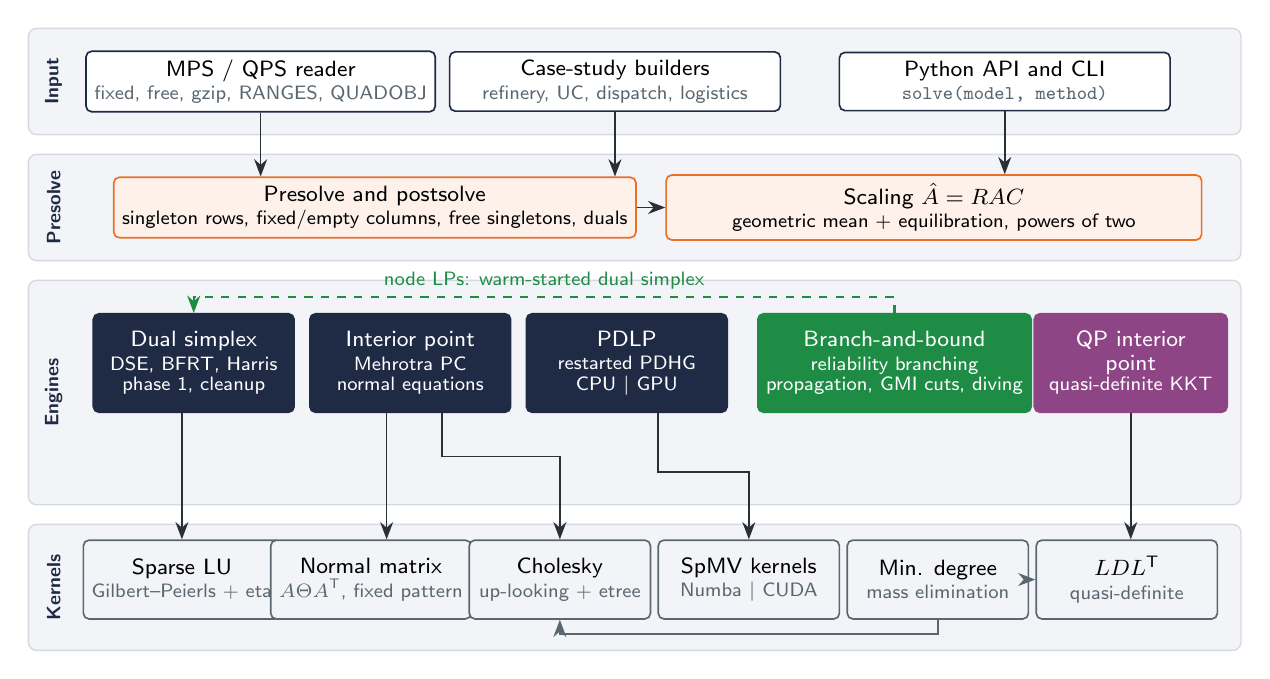
\begin{tikzpicture}[x=1cm,y=1cm]
  % layer bands
  \foreach \y/\h/\name in {0/1.35/Input, -1.6/1.35/Presolve, -3.2/2.85/Engines, -6.3/1.6/Kernels}{
    \draw[layer] (0,\y) rectangle (15.4,\y-\h);
    \node[rotate=90,font=\sffamily\scriptsize\bfseries,text=navy] at (0.32,\y-\h/2) {\name};
  }
  % input
  \node[blk,minimum width=3.9cm] (mps) at (2.95,-0.675) {MPS / QPS reader\\[-1pt]{\scriptsize\color{muted}fixed, free, gzip, RANGES, QUADOBJ}};
  \node[blk,minimum width=4.2cm] (cases) at (7.45,-0.675) {Case-study builders\\[-1pt]{\scriptsize\color{muted}refinery, UC, dispatch, logistics}};
  \node[blk,minimum width=4.2cm] (api) at (12.4,-0.675) {Python API and CLI\\[-1pt]{\scriptsize\color{muted}\code{solve(model, method)}}};
  % presolve
  \node[blks,minimum width=6.6cm] (pre) at (4.4,-2.275) {Presolve and postsolve\\[-1pt]{\scriptsize singleton rows, fixed/empty columns, free singletons, duals}};
  \node[blks,minimum width=6.8cm] (scal) at (11.5,-2.275) {Scaling $\hat A = RAC$\\[-1pt]{\scriptsize geometric mean + equilibration, powers of two}};
  % engines
  \node[blkn,minimum width=2.55cm,minimum height=1.25cm] (spx) at (2.1,-4.25) {Dual simplex\\[-1pt]{\scriptsize DSE, BFRT, Harris}\\[-2pt]{\scriptsize phase 1, cleanup}};
  \node[blkn,minimum width=2.55cm,minimum height=1.25cm] (ipm) at (4.85,-4.25) {Interior point\\[-1pt]{\scriptsize Mehrotra PC}\\[-2pt]{\scriptsize normal equations}};
  \node[blkn,minimum width=2.55cm,minimum height=1.25cm] (pdlp) at (7.6,-4.25) {PDLP\\[-1pt]{\scriptsize restarted PDHG}\\[-2pt]{\scriptsize CPU \textbar{} GPU}};
  \node[blk,draw=igreen,fill=igreen,text=white,minimum width=2.9cm,minimum height=1.25cm] (bnb) at (11.0,-4.25) {Branch-and-bound\\[-1pt]{\scriptsize reliability branching}\\[-2pt]{\scriptsize propagation, GMI cuts, diving}};
  \node[blk,draw=plum,fill=plum,text=white,minimum width=2.45cm,minimum height=1.25cm] (qp) at (14.0,-4.25) {QP interior\\[-1pt] point\\[-2pt]{\scriptsize quasi-definite KKT}};
  \draw[->,igreen,line width=0.8pt,dashed] (bnb.north) -- ++(0,0.2) -| node[pos=0.25,above,lbl,text=igreen,yshift=-1pt]{node LPs: warm-started dual simplex} (spx.north);
  % kernels, each under the engine that uses it
  \foreach \k/\x/\t/\s in {lu/1.95/Sparse LU/Gilbert--Peierls + eta,
                          nrm/4.35/Normal matrix/{$A\Theta A\T$, fixed pattern},
                          chol/6.75/Cholesky/up-looking + etree,
                          spmv/9.15/SpMV kernels/Numba \textbar{} CUDA,
                          amd/11.55/Min. degree/mass elimination,
                          ldl/13.95/$LDL\T$/quasi-definite}{
    \node[blkm,minimum width=2.3cm,minimum height=1.0cm] (\k) at (\x,-7.0) {\t\\[-1pt]{\scriptsize\color{muted}\s}};
  }
  % engine -> kernel
  \draw[flow] ([xshift=-1.5mm]spx.south) -- ([xshift=-1.5mm]spx.south |- lu.north);
  \draw[flow] ([xshift=-3mm]ipm.south) -- ([xshift=-3mm]ipm.south |- nrm.north);
  \draw[flow] ([xshift=4mm]ipm.south) -- ++(0,-0.55) -| (chol.north);
  \draw[flow] ([xshift=4mm]pdlp.south) -- ++(0,-0.75) -| (spmv.north);
  \draw[flow] (qp.south) -- (qp.south |- ldl.north);
  \draw[flow,muted] (amd.east) -- (ldl.west);
  \draw[flow,muted] (amd.south) -- ++(0,-0.18) -| (chol.south);
  % input -> presolve -> engines
  \draw[flow] (mps.south) -- (mps.south |- pre.north);
  \draw[flow] (cases.south) -- (cases.south |- pre.north);
  \draw[flow] (api.south) -- (api.south |- scal.north);
  \draw[flow] (pre.east) -- (scal.west);
\end{tikzpicture}
\caption[System architecture]{System architecture. Everything in the four bands is \nirnay{} code.
The dashed arrow shows that branch-and-bound solves its node LPs with the warm-started dual
simplex. Minimum degree orders both the Cholesky and the $LDL\T$ factorisations.}
\label{fig:arch}
\end{figure}

\begin{table}[tbp]
\centering\small
\caption[Solver modules]{Solver modules of \nirnay{} with their line counts (read from the
source files by \file{gen\_data.py}). The core solver is \locCore{} lines; the case-study builders
add \locCases{}.}
\label{tab:modules}
\begin{tabularx}{\linewidth}{@{}l r X@{}}
\toprule
Module (\file{nirnay/\dots}) & Lines & Role\\
\midrule
\rows{data/modules.tex}
\bottomrule
\end{tabularx}
\end{table}

\subsection{The path of a solve}
\Cref{fig:dataflow} follows one LP or MILP from file to answer. Each transformation on the way
in has an exact inverse on the way out, so the returned $x$, $y$ and $z$ satisfy the optimality
conditions \eqref{eq:kkt-lp} of the model in the file, not only those of the scaled, reduced
model the engine saw.

\begin{figure}[tbp]
\centering
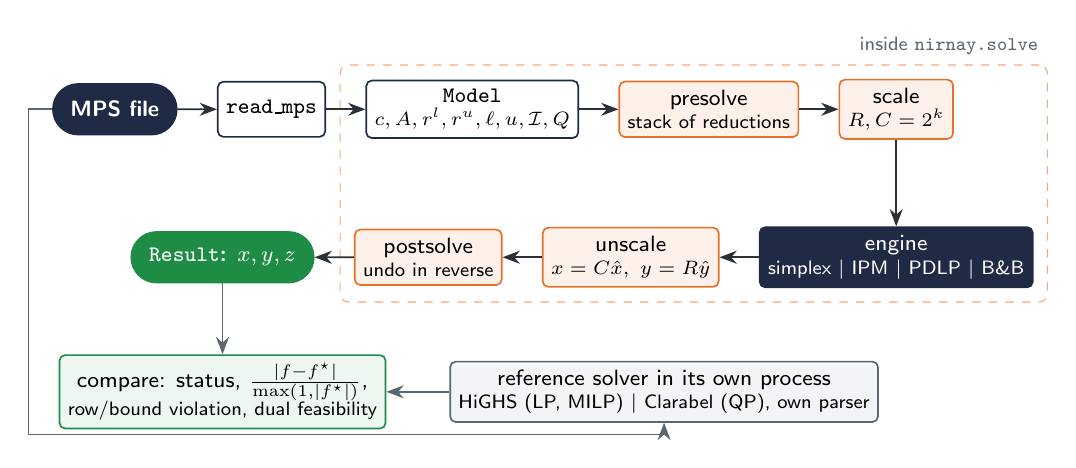
\begin{tikzpicture}[node distance=5mm and 5mm]
  \node[term] (file) {MPS file};
  \node[blk,right=of file] (read) {\code{read\_mps}};
  \node[blk,right=of read] (model) {\code{Model}\\[-1pt]{\scriptsize$c,A,r^l,r^u,\ell,u,\mathcal I,Q$}};
  \node[blks,right=of model] (pre) {presolve\\[-1pt]{\scriptsize stack of reductions}};
  \node[blks,right=of pre] (scale) {scale\\[-1pt]{\scriptsize$R,C=2^k$}};
  \node[blkn,below=11mm of scale,minimum width=2.6cm] (eng) {engine\\[-1pt]{\scriptsize simplex \textbar{} IPM \textbar{} PDLP \textbar{} B\&B}};
  \node[blks,left=of eng] (unscale) {unscale\\[-1pt]{\scriptsize$x=C\hat x,\ y=R\hat y$}};
  \node[blks,left=of unscale] (post) {postsolve\\[-1pt]{\scriptsize undo in reverse}};
  \node[term,fill=igreen,draw=igreen,left=of post] (res) {\code{Result}: $x,y,z$};
  \draw[flow] (file) -- (read);
  \draw[flow] (read) -- (model);
  \draw[flow] (model) -- (pre);
  \draw[flow] (pre) -- (scale);
  \draw[flow] (scale) -- (eng);
  \draw[flow] (eng) -- (unscale);
  \draw[flow] (unscale) -- (post);
  \draw[flow] (post) -- (res);
  % verification branch
  \node[blkg,below=9mm of res] (cmp) {compare: status, $\frac{|f-f^\star|}{\max(1,|f^\star|)}$,\\[-1pt]{\scriptsize row/bound violation, dual feasibility}};
  \node[blkm,right=8mm of cmp] (ref) {reference solver in its own process\\[-1pt]{\scriptsize HiGHS (LP, MILP) \textbar{} Clarabel (QP), own parser}};
  \draw[flow,muted] (file.west) -- ++(-0.3,0) |- ([yshift=-1.5mm]ref.south) -- (ref.south);
  \draw[flow,muted] (res.south) -- (cmp.north);
  \draw[flow,muted] (ref) -- (cmp);
  \begin{scope}[on background layer]
    \node[fit=(pre)(scale)(eng)(unscale)(post),draw=saffron!60,dashed,rounded corners=3pt,inner sep=5pt,
          label={[lbl,anchor=south east]north east:inside \code{nirnay.solve}}] {};
  \end{scope}
\end{tikzpicture}
\caption[Data flow of a solve]{Data flow of a solve. The upper row reduces and scales the model.
The engine solves it, and the lower row maps the solution back. The benchmark harness (bottom)
re-solves the same file with a reference solver in a separate process and checks the answer.}
\label{fig:dataflow}
\end{figure}

\subsection{Input: the MPS/QPS reader}
\file{nirnay/io/mps.py} reads fixed and free MPS, gzip-compressed files, \code{OBJSENSE},
integer \code{MARKER} blocks, \code{RANGES}, the bound types \code{UP LO FX FR MI PL BV LI UI},
an objective constant given as the RHS of the objective row, and the QP sections \code{QUADOBJ}
(one triangle), \code{QMATRIX} and \code{QSECTION} (both triangles). It follows the conventions the
benchmark libraries assume: an integer column in a \code{MARKER} block without bounds gets
$[0,\infty)$; \code{UP} with a negative value on a column whose lower bound is still $0$ sets
the lower bound to $-\infty$; \code{RANGES} on an equality row extend upward for $R>0$ and
downward for $R<0$; the objective constant is minus the RHS of the objective row. Fixed-format
files whose names contain spaces (Netlib's \code{forplan}) are detected and parsed by column
position. The earliest interior-point sweep failed to read \code{forplan} and \code{standgub}
(\cref{tab:fixes-ipm}); both read correctly now. A writer (\file{io/mps\_write.py}) emits
free MPS. Read, write and re-read reproduce the arrays of the benchmark files, and HiGHS reads the
original and the written file into the same model (\cref{sec:verification}).

\subsection{Scaling}\label{sec:scaling}
Industrial models mix units (tonnes, kilolitres, rupees, percentages), so the coefficients of
$A$ span many orders of magnitude and every factorisation loses digits to that spread.
\file{presolve/scaling.py} computes diagonal $R$ and $C$ and solves the scaled problem with
$\hat A=RAC$, $\hat c=Cc$, $\hat r = R r$ and $\hat\ell = C^{-1}\ell$, $\hat u = C^{-1}u$, in two
stages~\cite{elble2012}:
\begin{enumerate}
  \item \textbf{Geometric-mean passes.} Divide each row, then each column, by
        $\sqrt{\max_j|\hat a_{ij}|\cdot\min_j|\hat a_{ij}|}$. Stop after 8 passes, or earlier once
        a pass reduces the overall spread $\max|\hat a|/\min|\hat a|$ by less than 10\%. Entries
        below $10^{-12}$ of the largest in their row or column are left out of the minimum: they
        carry no information in double precision, but a geometric mean would let them dominate.
        The QP \code{KSIP} has an entry of order $10^{-30}$ next to entries of order~1, and scaling by
        it ruined every other entry of its line.
  \item \textbf{Equilibration.} A final column pass makes the largest entry of every column
        exactly~1.
\end{enumerate}
Each factor is then rounded to the nearest power of two, $R_i \leftarrow 2^{\operatorname{round}(\log_2 R_i)}$.
Multiplying by a power of two changes only the floating-point exponent, so scaling adds no rounding
error of its own, and unscaling ($x=C\hat x$, $y=R\hat y$, $z=C^{-1}\hat z$) returns exactly the
numbers the engine computed. PDLP uses its own preconditioner (Ruiz and Pock--Chambolle,
\cref{sec:pdlp}), because the convergence rate of a first-order method depends on the conditioning
of $A$ in a different way.

% Section 4: presolve and postsolve.
\section{Presolve and postsolve}\label{sec:presolve}

Presolve shrinks a model before any engine sees it. The reductions in
\file{nirnay/presolve/presolve.py} are the classical ones of Andersen and Andersen~\cite{andersen1995}
and Gondzio~\cite{gondzio1997}, restricted to those with an \emph{exact primal and dual}
postsolve. Postsolve therefore returns duals $y$ and reduced costs $z$ for the original model as
well as~$x$. \code{nirnay.solve} applies presolve by default to LPs and MILPs solved by the simplex,
the interior-point method and branch-and-bound. It is not applied to QPs or to PDLP, which works on the
original rows.

\subsection{Reductions}
Presolve runs over columns and rows repeatedly until a pass changes nothing (at most 20 passes). Every
reduction pushes a record onto a stack; postsolve pops the stack. With $\bar c$ the current
(possibly modified) cost vector and $[\bar r^l,\bar r^u]$ the current row bounds:

\begin{description}[style=nextline,leftmargin=1.2em,font=\sffamily\bfseries\color{navy}]
\item[Fixed column] ($\ell_j=u_j$). Substitute $x_j=\ell_j$: $\bar r\leftarrow \bar r - a_j\ell_j$,
  $c_0\leftarrow c_0+\bar c_j\ell_j$. Postsolve: $x_j=\ell_j$; $z_j$ follows from the final $y$.
\item[Empty column] (no nonzero in any live row). Set $x_j$ to the bound its cost prefers:
  $\ell_j$ if $\bar c_j>0$, $u_j$ if $\bar c_j<0$. If that bound is infinite the problem is
  unbounded. Postsolve: $z_j=\bar c_j$.
\item[Empty row] Drop it, or declare infeasibility if $0\notin[\bar r^l_i,\bar r^u_i]$. Postsolve: $y_i=0$.
\item[Redundant row] If the activity bounds $L_i=\sum_j \min(a_{ij}\ell_j,a_{ij}u_j)$ and
  $U_i=\sum_j\max(a_{ij}\ell_j,a_{ij}u_j)$ lie inside $[\bar r^l_i,\bar r^u_i]$, the row can never
  bind: drop it, $y_i=0$. If $[L_i,U_i]$ misses the row interval the problem is infeasible.
\item[Singleton row] ($a_{ij}x_j\in[\bar r^l_i,\bar r^u_i]$ with one live entry). The row becomes
  a bound on $x_j$:
  \begin{equation}\label{eq:singleton-bound}
     \ell_j \leftarrow \max\bigl(\ell_j,\; \lambda\bigr),\quad u_j\leftarrow \min\bigl(u_j,\;\mu\bigr),\qquad
     [\lambda,\mu] = \begin{cases} [\bar r^l_i/a_{ij},\ \bar r^u_i/a_{ij}] & a_{ij}>0,\\
                                   [\bar r^u_i/a_{ij},\ \bar r^l_i/a_{ij}] & a_{ij}<0,\end{cases}
  \end{equation}
  rounded inward for an integer column. The record keeps which of the two bounds the row
  supplied, and (see \cref{sec:presolve-bug}) the column's cost $\bar c_j$ and its live rows at this moment.
\item[Free column singleton] on an equality row. If $x_j$ appears only in row $i$, the row is
  $\sum_k a_{ik}x_k = b_i$, and the bounds of $x_j$ cannot bind (it is free, or the row and the
  other columns' bounds imply its bounds), then $x_j$ can be eliminated with the row:
  \begin{equation}\label{eq:free-singleton}
    x_j = \frac{b_i-\sum_{k\ne j}a_{ik}x_k}{a_{ij}},\qquad
    y_i = \frac{\bar c_j}{a_{ij}},\qquad
    \bar c_k \leftarrow \bar c_k - a_{ik}\,y_i\ (k\ne j),\qquad c_0\leftarrow c_0 + b_i\,y_i .
  \end{equation}
  The dual is known at removal time, because $x_j$ is basic (it is not at a bound), so its reduced
  cost $\bar c_j - a_{ij}y_i$ must be zero.
\item[Integer bounds] (MILP only). Round integer bounds inward and tighten them by
  activity-based propagation over the live rows (\cref{sec:propagation}); see
  Achterberg et al.~\cite{achterberg2020} for the MIP presolve reductions still missing. The LP dual is not needed
  for a MILP, so these reductions need no dual postsolve.
\end{description}

\subsection{Postsolve and dual recovery}
Postsolve starts from the reduced solution: $x$ on kept columns, $x_j$ of removed columns as
recorded, $y$ on kept rows and $y_i=0$ on removed rows. It maintains $z=c-A\T y$ over the
\emph{original} model and undoes the stack in reverse order:
\begin{itemize}
  \item a free column singleton restores $x_j$ and sets $y_i=\bar c_j/a_{ij}$ from \eqref{eq:free-singleton};
  \item a singleton row computes the reduced cost of $x_j$ \emph{in the problem as it was when
    the row was removed},
    \begin{equation}\label{eq:zbar}
      \bar z_j = \bar c_j^{\,\text{rec}} - \sum_{k\in\mathcal{R}_j^{\text{rec}}} a_{kj}\,y_k ,
    \end{equation}
    where $\bar c_j^{\,\text{rec}}$ and $\mathcal{R}_j^{\text{rec}}$ (the rows in which $x_j$ was
    still live) were recorded at removal. If the bound this row created is active and $\bar z_j$
    has the sign that bound can absorb, the reduced cost moves to the row:
    \begin{equation}\label{eq:singleton-dual}
      \bigl(x_j=\lambda \text{ and } \bar z_j>0\bigr)\ \text{or}\ \bigl(x_j=\mu\text{ and }\bar z_j<0\bigr)
      \quad\Longrightarrow\quad y_i = \frac{\bar z_j}{a_{ij}},\qquad z_j\leftarrow z_j - a_{ij}y_i .
    \end{equation}
    Otherwise $y_i=0$ and the bound's multiplier stays in~$z_j$.
  \item empty, redundant and fixed items need nothing: $y_i=0$, and $z_j$ is already correct.
\end{itemize}
Each assignment of $y_i$ subtracts $a_{i\cdot}y_i$ from the running $z$, so at the end
$z=c-A\T y$ holds exactly and \eqref{eq:kkt-lp} can be checked on the original model.

\subsection{An order-dependence bug in singleton-row duals}\label{sec:presolve-bug}
\begin{lessonbox}[Bug: singleton-row duals depended on the order of undoing]
\textbf{Symptom.} With presolve switched on, some postsolved solutions had an optimal $x$ but duals
that violated the sign conditions \eqref{eq:kkt-lp} of the original model. The violations sat on
columns that had lost singleton rows, and they depended on the order in which the reductions were
undone.

\textbf{Cause.} The first version decided \eqref{eq:singleton-dual} from the running reduced cost
$z_j = c_j - \sum_k a_{kj}y_k$ at the moment the record was undone. That value is wrong in two ways:
\begin{enumerate}[leftmargin=1.4em]
  \item it uses the original $c_j$, while the reduced problem that removed the row had cost
        $\bar c_j$, already modified by free-column-singleton substitutions
        \eqref{eq:free-singleton} made \emph{earlier};
  \item it sums over all rows of $x_j$, including rows removed \emph{before} this one. Their duals
        are assigned \emph{later} in postsolve (the stack is undone in reverse), so they are still
        zero. Another singleton row on the same column is the typical case.
\end{enumerate}
Both errors depend on the order of reductions, so the answer depended on that order too.

\textbf{Fix.} Record $\bar c_j$ and the live rows of column $j$ (indices and coefficients) when
the row is removed, and evaluate \eqref{eq:zbar} from the record. Every row in
$\mathcal{R}_j^{\text{rec}}$ is either kept (its dual comes from the engine) or removed
\emph{after} this row, and so undone \emph{before} it. Its dual is therefore final when
\eqref{eq:zbar} is evaluated. By induction over the stack, each undo step turns an optimal
primal--dual pair of the smaller problem into one of the larger problem.
\end{lessonbox}

The simplex was changed at the same time to recompute $y=B\mT c_B$ exactly for the true costs
when it returns an optimal basis (\file{lp/simplex.py}, \code{\_result}). Its iteration loop
updates reduced costs incrementally and refreshes $y$ only at refactorisation, and the dual
loop may shift costs (\cref{sec:simplex-safeguards}), so the $y$ held at the end is not exactly the
dual of the final basis for the original costs. Postsolve needs exact duals.

\ifnum\haveDualCheck=1
\paragraph{Check} \file{tools/dual\_check.py} solves every Netlib LP with presolve and the dual
simplex (\SI{60}{s} limit) and tests primal feasibility and the sign conditions
\eqref{eq:kkt-lp} on the original model, relative to $1+\|c\|_\infty$. On the run used for this
report, \nDualOk{} of \nDualTot{} problems passed with \nDualBad{} failures. The largest relative
reduced-cost violation was \dualMaxZ{} and the largest row-dual sign violation \dualMaxY{}. The remaining
\nDualStatus{} problems, \dualStatusNames, hit the \SI{60}{s} limit of the check and were not tested.
\fi

\subsection{What presolve removes}
\ifnum\haveCensus=1
Running presolve alone on the \nCensus{} Netlib problems removes \censusRowsPct\% of all rows,
\censusColsPct\% of all columns and \censusNnzPct\% of all nonzeros (median \censusMedRowsPct\% of
rows per problem, up to \censusMaxRowsPct\% on \code{\censusMaxRowsName}). \censusUntouched{}
problems are not reduced at all. \Cref{tab:presolve-rules} counts the reductions by rule. The whole
census takes \censusTime\,s, with \code{\censusMaxTimeName} the slowest at \censusMaxTime\,s, because
presolve is written in plain Python loops.

\begin{table}[ht]
\centering\small
\caption[Presolve reductions on Netlib]{Presolve reductions on the Netlib LPs, by rule: how many
rows or columns each rule removed in total, and on how many problems it fired at least once.}
\label{tab:presolve-rules}
\begin{tabular}{@{}lrr@{}}
\toprule
Rule & Removed & Problems\\
\midrule
\rows{data/presolve_rules.tex}
\bottomrule
\end{tabular}
\end{table}
\fi

These are only the simplest reductions. The comparator study (\cref{sec:competitors}) shows that
doubleton equations, forcing rows, dominated columns and parallel rows account for most of what
HiGHS's presolve removes. Those are next on the roadmap (\cref{sec:roadmap}).

\ifnum\haveSpxPresolve=1
\paragraph{Effect on the dual simplex}
The simplex sweep with presolve is \file{\presolveFile}\ifnum\presolvePartial=1{}, which was still
running when this report was built, with \presolveDone{} of the \nNetlibFiles{} Netlib problems
finished\fi. It solves \presolveSolved{} of its \presolveDone{} problems (failures: \presolveFailNames). On the
\nPresolveCommon{} problems solved both with and without presolve, presolve reduces the dual
iterations by a factor of \presolveIterRatio{} (geometric mean of the ratios). Timed against HiGHS
inside each sweep, which cancels differences in machine load between the two runs, the shifted-mean
ratio is \presolveRatioHighs{} with presolve and \presolveRatioHighsVtwo{} without, and the geometric
mean of per-instance ratios is \presolveGmrHighsCommon{} with presolve and
\presolveGmrHighsCommonVtwo{} without.
(The raw times are not comparable: HiGHS itself ran \presolveLoad{} times slower, in geometric mean,
during the sweep with presolve, because other sweeps shared the machine.)
\ifnum\presolveFaster=1 Presolve therefore pays for itself on these problems.\fi
\ifnum\presolveFaster=0 Presolve therefore roughly breaks even in shifted geometric mean, which weights
the longer solves\ifnum\presolveSmallWorse=1, and it costs time on the many small problems, where the
per-instance ratio rises\fi. Its passes are pure Python loops, which on small problems cost about as
much as the iterations they save, or more. Compiling presolve is part of the first roadmap item, and
the payoff should come from the stronger reductions still to be written.\fi
\ifnum\presolveFaster=-1 Presolve therefore does not yet pay for itself. Its passes are pure Python
loops, and on these small problems they cost more than the iterations they save. Compiling presolve is
part of the first roadmap item.\fi
\fi

% Section 5: sparse linear algebra.
\section{Sparse linear algebra}\label{sec:linalg}

Every engine except PDLP spends most of its time solving linear systems: the simplex with the basis
matrix $B$, the LP interior-point method with the normal matrix $M=B\Theta B\T$, and the QP method with
the augmented matrix $K$. \nirnay{} implements the three factorisations it needs and the
fill-reducing ordering they share. All numeric kernels are Numba-compiled loops over plain CSC
arrays.

\subsection{Sparse LU of the simplex basis}\label{sec:lu}
\file{linalg/lu.py} factorises $BQ=\tilde L U$, where $Q$ is a column order, $U$ is upper
triangular in pivot order, and $\tilde L$ is unit lower triangular up to a row permutation (column
$k$ of $\tilde L$ has its unit entry at the pivot row $p_k$).

\paragraph{Column order}
A simplex basis is mostly triangular, and the order exploits that (Suhl and Suhl~\cite{suhl1990}).
A linear-time pass over the basis repeatedly removes \emph{column singletons} of the active
submatrix (logical columns are the first of them), then \emph{row singletons}; each removal can
create new singletons. What is left is the \emph{bump}, ordered by increasing active column count.
Each triangular column is given the singleton row found for it as its pivot, and the factorisation
takes the columns in the order column singletons, row singletons (in the order found), bump. In
the left-looking scheme below, a row-singleton row is touched by no later column, so its column of
$\tilde L$ is never applied again. All fill is therefore confined to the bump. On final Netlib bases
this lowers $(\nnz(\tilde L)+\nnz(U))/\nnz(B)$ from 2.95 to 1.81 on \code{d2q06c}, 2.47 to 1.80 on
\code{25fv47} and 1.24 to 1.06 on \code{degen3}; \code{pilot}, whose bump is large and dense, stays
near 7 and needs a genuine Markowitz factorisation of the bump.

\paragraph{Left-looking elimination}
Column $k$ is computed by the sparse triangular solve of Gilbert and Peierls~\cite{gilbert1988}:
\begin{equation}\label{eq:gp}
  \tilde L_{:,1:k-1}\, x = B_{:,q_k},
\end{equation}
where only columns of $\tilde L$ already computed take part. The rows that become nonzero in
$x$ are exactly the nodes reachable from the nonzeros of $B_{:,q_k}$ in the graph of $\tilde L$. An
iterative depth-first search finds them in topological order, so the numeric solve touches only
those rows. The work is proportional to the floating-point operations, not to~$m$. Entries of $x$
in already-pivoted rows form column $k$ of~$U$; the others are the candidates for the pivot.

\paragraph{Threshold pivoting}
A triangular column takes its assigned singleton row whenever that entry passes the threshold test.
Otherwise, among unpivoted rows $r$ with $|x_r|\ge\tau\max_{r'}|x_{r'}|$ ($\tau=0.1$), the pivot is
the row with the fewest nonzeros inside the bump, with ties broken by magnitude. This is Markowitz's idea
\cite{markowitz1957} applied row-wise: it gives up a little stability for much less fill.

\paragraph{Basis repair}
If no candidate exceeds $10^{-11}$, column $q_k$ depends on the columns before it. Rather than
reject the basis, the factorisation leaves step $k$ unpivoted and reports a pair (basis position,
unpivoted row). The simplex then swaps that basic variable for the row's logical, which is always
independent of the rest, and refactorises. Near-singular bases arise from rounding and from
degenerate pivots on models such as the \code{pilot} family, and industrial simplex codes keep
going the same way.

\paragraph{Updates}
After a pivot that replaces basis position $r$ by a column with $\alpha_q=B^{-1}a_q$, the new inverse
is $B_{\text{new}}^{-1}=E^{-1}B^{-1}$ with the elementary eta matrix
\begin{equation}\label{eq:eta}
  E = I + (\alpha_q - e_r)e_r\T,\qquad
  E^{-1}v = v - \frac{v_r}{\alpha_{q,r}}(\alpha_q - e_r) ,
\end{equation}
the product form of the inverse~\cite{dantzig1954}. The eta file stores $\alpha_q$ sparsely,
dropping entries below $10^{-14}$. FTRAN ($B x = b$) applies the LU solve and then the etas in order;
BTRAN ($B\T y=d$) applies the etas in reverse and then the transposed LU solve. For that
solve the factorisation also keeps row-wise copies of $\tilde L$ and $U$, so both triangular solves
run in the axpy form that skips zero entries; the right-hand side $e_r$ of the simplex's BTRAN
is very sparse, and the column-wise dot-product form could not exploit that. The basis is
refactorised after 100 updates, or earlier when the eta file holds more than
$8(\nnz(\tilde L)+\nnz(U)+m)$ entries, to bound both the work per solve and the growth of rounding
error.

\begin{algorithm}[t]
\caption{Left-looking sparse LU with threshold pivoting and repair (\file{linalg/lu.py})}\label{alg:lu}
\Input{basis $B$ (CSC), column order $q$, row counts $\rho_r$, threshold $\tau$, tiny $\epsilon$}
\Output{$\tilde L$, $U$, pivot rows $p$, list of unpivoted steps}
\For{$k=1,\dots,m$}{
  $\mathcal{X}\leftarrow$ reach of $\operatorname{struct}(B_{:,q_k})$ in the graph of $\tilde L$, in topological order (DFS)\;
  scatter $x\leftarrow B_{:,q_k}$; \ForEach{$r\in\mathcal X$ with $r$ pivoted at step $s$}{$x_{\mathcal{L}_s}\leftarrow x_{\mathcal{L}_s}-\tilde L_{\mathcal{L}_s,s}\,x_r$}
  $U_{:,k}\leftarrow\{x_r : r \text{ pivoted}\}$;\quad $a_{\max}\leftarrow\max\{|x_r|: r\text{ unpivoted}\}$\;
  \eIf{$a_{\max}>\epsilon$}{
    $p_k\leftarrow\arg\min\{\rho_r : r \text{ unpivoted},\ |x_r|\ge\tau a_{\max}\}$ \Comment*[r]{shortest row}
    $U_{kk}\leftarrow x_{p_k}$;\quad $\tilde L_{:,k}\leftarrow x_{\text{unpivoted}}/x_{p_k}$\;
  }{
    record step $k$ as singular \Comment*[r]{caller swaps in a logical}
  }
  clear $x$ on $\mathcal X$\;
}
\end{algorithm}

\subsection{Sparse Cholesky for the normal equations}\label{sec:chol}
The LP interior-point method solves $M\,\Delta y=r$ with $M=B\Theta B\T+\delta I$ symmetric
positive definite and the same sparsity pattern at every iteration. \file{linalg/cholesky.py}
splits the work in the classic way~\cite{davis2006}:
\begin{enumerate}
  \item \textbf{Analyse} once. Compute a fill-reducing permutation $P$ (\cref{sec:ordering}), the
        upper triangle of $PMP\T$ with a map back to $M$'s values, the elimination tree
        ($\operatorname{parent}(i)=\min\{k>i: l_{ki}\ne0\}$, computed with path compression), and
        the column counts of $L$ from the row subtrees. $L$'s pattern is then allocated exactly.
  \item \textbf{Factor} every iteration, by the up-looking algorithm. Row $k$ of $L$ solves
        \begin{equation}\label{eq:uplook}
          L_{1:k-1,1:k-1}\; l_{k} = m_{1:k-1,k},\qquad
          L_{kk} = \sqrt{m_{kk} - l_k\T l_k},
        \end{equation}
        and the nonzeros of $l_k$ are the nodes on the paths from the nonzeros of $m_{1:k-1,k}$
        up the elimination tree to $k$ (the row subtree).
  \item \textbf{Solve} $LL\T\hat x = P b$ by forward and back substitution.
\end{enumerate}

\paragraph{Pivot guard}
As the interior-point iterates converge, $M$ becomes nearly singular: rows may be dependent,
and $\Theta$ spans many orders of magnitude. If the pivot $m_{kk}-l_k\T l_k\le 10^{-30}$, it is
replaced by $10^{128}$. The corresponding component of the solution then becomes (almost) zero
instead of overflowing, which is the standard remedy~\cite[§11.1]{wright1997}. The number of
replaced pivots is reported with each factorisation.

\subsection{Minimum-degree ordering and fill-in}\label{sec:ordering}
Eliminating a node of the graph of a symmetric matrix joins all its neighbours into a clique, and
the new edges are exactly the fill-in of~$L$. \file{linalg/ordering.py} implements the minimum-degree
heuristic~\cite{tinney1967,george1989}: it repeatedly eliminates a node of smallest current degree,
on an explicit elimination graph with degree buckets. Two refinements matter on optimisation
matrices:
\begin{itemize}
  \item \textbf{mass elimination:} neighbours whose closed neighbourhood equals the pivot's would each
        be chosen next anyway, so they are eliminated together. This removes most of the cost on
        block-structured matrices;
  \item \textbf{dense-row deferral:} nodes with degree above $\max(16,10\sqrt n)$ are taken out of the
        graph and ordered last. Normal matrices of LPs often have a few almost-dense rows, and
        ordering them last both bounds the work of the ordering and keeps the dense part of $L$ in
        the final block.
\end{itemize}
\Cref{fig:fill} shows why the order matters on the smallest example, an arrowhead matrix.

\begin{figure}[tbp]
\centering
\newcommand{\cell}[3]{\fill[#3] ({(#2-1)*0.42},{-(#1-1)*0.42}) rectangle ++(0.36,-0.36);}
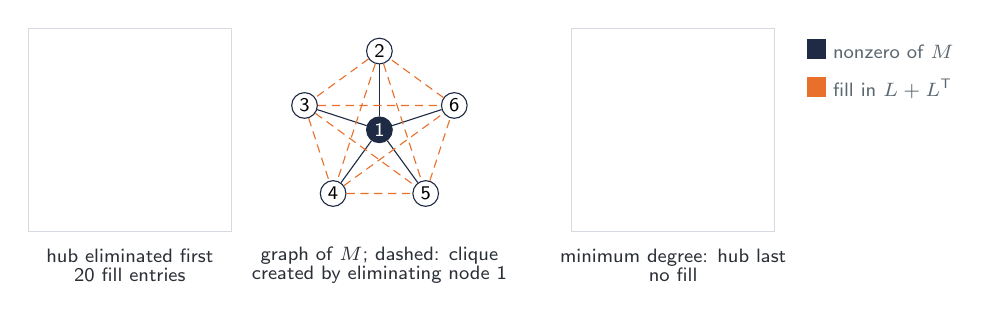
\begin{tikzpicture}
  % ---- left: hub first
  \begin{scope}
    \draw[rule] (-0.06,0.06) rectangle (2.52,-2.52);
    \foreach \i in {1,...,6}{\cell{\i}{\i}{navy}}
    \foreach \j in {2,...,6}{\cell{1}{\j}{navy}\cell{\j}{1}{navy}}
    \foreach \i in {2,...,6}{\foreach \j in {2,...,6}{\ifnum\i=\j\else\cell{\i}{\j}{saffron}\fi}}
    \node[lbl,text=ink,align=center] at (1.23,-2.95) {hub eliminated first\\[-1pt]20 fill entries};
  \end{scope}
  % graph in the middle
  \begin{scope}[shift={(4.4,-1.23)}]
    \node[circle,draw=navy,fill=navy,text=white,inner sep=1.2pt,font=\sffamily\scriptsize] (h) at (0,0) {1};
    \foreach \k/\a in {2/90,3/162,4/234,5/306,6/18}{
      \node[circle,draw=navy,fill=white,inner sep=1.2pt,font=\sffamily\scriptsize] (n\k) at (\a:1.0) {\k};
      \draw[navy] (h) -- (n\k);}
    \draw[saffron,densely dashed] (n2)--(n3) (n3)--(n4) (n4)--(n5) (n5)--(n6) (n6)--(n2) (n2)--(n4) (n2)--(n5) (n3)--(n5) (n3)--(n6) (n4)--(n6);
    \node[lbl,text=ink,align=center] at (0,-1.72) {graph of $M$; dashed: clique\\[-1pt]created by eliminating node 1};
  \end{scope}
  % ---- right: hub last (minimum degree)
  \begin{scope}[shift={(6.9,0)}]
    \draw[rule] (-0.06,0.06) rectangle (2.52,-2.52);
    \foreach \i in {1,...,6}{\cell{\i}{\i}{navy}}
    \foreach \j in {1,...,5}{\cell{6}{\j}{navy}\cell{\j}{6}{navy}}
    \node[lbl,text=ink,align=center] at (1.23,-2.95) {minimum degree: hub last\\[-1pt]no fill};
  \end{scope}
  \node[lbl,anchor=west] at (9.7,-0.2) {\tikz\fill[navy] (0,0) rectangle (0.25,0.25); nonzero of $M$};
  \node[lbl,anchor=west] at (9.7,-0.7) {\tikz\fill[saffron] (0,0) rectangle (0.25,0.25); fill in $L+L\T$};
\end{tikzpicture}
\caption[Fill-in and ordering]{Fill-in and ordering on an arrowhead matrix. Eliminating the hub
first (left) makes its five neighbours a clique (middle), and $L$ becomes dense. Minimum degree
eliminates the leaves first and the hub last (right), and $L$ has no fill at all. The same effect,
on a large scale, decides whether the normal matrix of an LP can be factorised at all.}
\label{fig:fill}
\end{figure}

\subsection{Assembling the normal matrix}\label{sec:normal}
$M = B\Theta B\T + \diag(\delta)$ changes its values at every interior-point iteration but not its
pattern. \file{linalg/normal.py} therefore computes once the full pattern of $BB\T$ (with sorted
row indices) and a \emph{slot map}. For each row $k$ of $B$, each column $j$ in that row, and each
entry $i$ of column $j$, the map gives the position of $M_{ik}$ in the value array. Each
iteration then assembles $M$ in one pass,
\begin{equation}\label{eq:assemble}
  M_{\text{slot}(q)} \mathrel{+}= \theta_j\, b_{kj}\, b_{ij},\qquad q=1,2,\dots,\ \sum_j \nnz(b_j)^2 ,
\end{equation}
with no searching and no allocation, followed by the diagonal term $\delta_k$.

\subsection{Quasi-definite \texorpdfstring{$LDL\T$}{LDLT} for the QP augmented system}\label{sec:ldl}
The QP method solves systems with the regularised augmented matrix
\begin{equation}\label{eq:qd}
  K=\begin{bmatrix} -H & B\T\\ B & R\end{bmatrix},\qquad H = Q+D+\rho I\succ0,\quad R=\delta I\succ0,
\end{equation}
which is symmetric \emph{quasi-definite}. Vanderbei~\cite{vanderbei1995} showed that such a matrix
has a factorisation $PKP\T=LDL\T$ with $D$ diagonal, $n$ negative and $m$ positive pivots, for
\emph{every} symmetric permutation $P$. The ordering can therefore be chosen for sparsity alone,
exactly as for Cholesky, and no pivoting for stability is needed during the numeric
factorisation. \file{linalg/ldl.py} reuses the Cholesky analysis (minimum degree, elimination tree,
column counts) and the up-looking $LDL\T$ kernel of Davis~\cite{davis2005}. The numeric step computes,
for row $k$,
\begin{equation}\label{eq:ldl}
  L_{kj} = \frac{y_j}{D_{jj}},\qquad D_{kk} = k_{kk} - \sum_{j<k} L_{kj}\,y_j ,
\end{equation}
where $y$ solves the sparse triangular system for row $k$.

\paragraph{Pivot floor}
The signs of the pivots are known in advance: $\sigma_k=-1$ for a primal row of $K$ and $+1$ for a
dual row. A pivot with the wrong sign, or smaller than $\delta_{\min}$ in magnitude, is replaced by
$\sigma_k\delta_{\min}$ (dynamic regularisation, with $\delta_{\min}=10^{-11}$ in the QP method). The
factorisation then always exists and has the correct inertia. The perturbation is removed by
iterative refinement against the unregularised matrix (\cref{sec:qp}). \Cref{fig:kkt} shows the
block structure.

\begin{figure}[tbp]
\centering
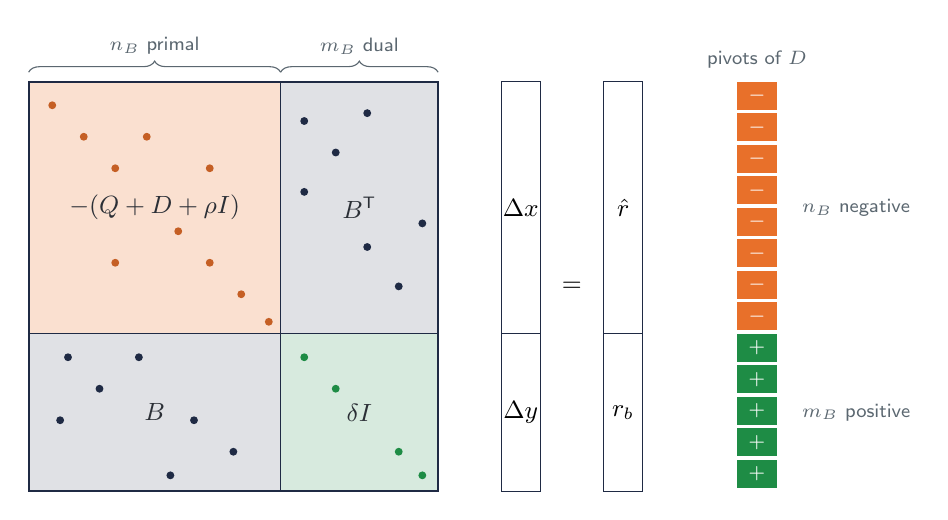
\begin{tikzpicture}[x=1cm,y=1cm]
  % K blocks
  \fill[saffron!22] (0,0) rectangle (3.2,-3.2);
  \fill[navy!14] (3.2,0) rectangle (5.2,-3.2);
  \fill[navy!14] (0,-3.2) rectangle (3.2,-5.2);
  \fill[igreen!18] (3.2,-3.2) rectangle (5.2,-5.2);
  \draw[navy,line width=0.7pt] (0,0) rectangle (5.2,-5.2);
  \draw[navy,line width=0.4pt] (3.2,0) -- (3.2,-5.2) (0,-3.2) -- (5.2,-3.2);
  % sparsity motif
  \foreach \p in {(0.3,-0.3),(0.7,-0.7),(1.1,-1.1),(1.5,-1.5),(1.9,-1.9),(2.3,-2.3),(2.7,-2.7),(3.05,-3.05),
                  (0.7,-1.5),(1.5,-0.7),(1.1,-2.3),(2.3,-1.1)}{\fill[saffron!85!black] \p circle (0.05);}
  \foreach \p in {(3.5,-3.5),(3.9,-3.9),(4.3,-4.3),(4.7,-4.7),(5.0,-5.0)}{\fill[igreen] \p circle (0.05);}
  \foreach \p in {(3.5,-0.5),(3.5,-1.4),(3.9,-0.9),(4.3,-2.1),(4.7,-2.6),(5.0,-1.8),(4.3,-0.4),
                  (0.5,-3.5),(1.4,-3.5),(0.9,-3.9),(2.1,-4.3),(2.6,-4.7),(1.8,-5.0),(0.4,-4.3)}{\fill[navy] \p circle (0.05);}
  \node[font=\small,text=ink,fill=saffron!22,inner sep=2pt] at (1.6,-1.6) {$-(Q+D+\rho I)$};
  \node[font=\small,text=ink,fill=navy!14,inner sep=2pt] at (4.2,-1.6) {$B\T$};
  \node[font=\small,text=ink,fill=navy!14,inner sep=2pt] at (1.6,-4.2) {$B$};
  \node[font=\small,text=ink,fill=igreen!18,inner sep=2pt] at (4.2,-4.2) {$\delta I$};
  % dimension braces
  \draw[decorate,decoration={brace,amplitude=4pt},muted] (0,0.12) -- node[above=3pt,lbl]{$n_B$ primal} (3.2,0.12);
  \draw[decorate,decoration={brace,amplitude=4pt},muted] (3.2,0.12) -- node[above=3pt,lbl]{$m_B$ dual} (5.2,0.12);
  % solution / rhs
  \draw[navy] (6.0,0) rectangle (6.5,-5.2); \draw[navy] (6.0,-3.2) -- (6.5,-3.2);
  \node[font=\small] at (6.25,-1.6) {$\Delta x$}; \node[font=\small] at (6.25,-4.2) {$\Delta y$};
  \node[font=\small] at (6.9,-2.6) {$=$};
  \draw[navy] (7.3,0) rectangle (7.8,-5.2); \draw[navy] (7.3,-3.2) -- (7.8,-3.2);
  \node[font=\small] at (7.55,-1.6) {$\hat r$}; \node[font=\small] at (7.55,-4.2) {$r_b$};
  % D signs
  \begin{scope}[shift={(9.0,0)}]
    \node[lbl,anchor=south] at (0.25,0.05) {pivots of $D$};
    \foreach \k in {0,...,7}{\fill[saffron] (0,-\k*0.4) rectangle (0.5,-\k*0.4-0.36); \node[font=\sffamily\scriptsize,text=white] at (0.25,-\k*0.4-0.18) {$-$};}
    \foreach \k in {0,...,4}{\fill[igreen] (0,-3.2-\k*0.4) rectangle (0.5,-3.2-\k*0.4-0.36); \node[font=\sffamily\scriptsize,text=white] at (0.25,-3.2-\k*0.4-0.18) {$+$};}
    \node[lbl,align=left,anchor=west] at (0.7,-1.6) {$n_B$ negative};
    \node[lbl,align=left,anchor=west] at (0.7,-4.2) {$m_B$ positive};
  \end{scope}
\end{tikzpicture}
\caption[Quasi-definite KKT block structure]{Block structure of the regularised augmented
(KKT) system solved at every QP interior-point iteration. The $(1,1)$ block is negative definite,
because it contains the barrier term $D=Z X^{-1}+S W^{-1}$ and the regularisation $\rho I$, and the
$(2,2)$ block is positive definite. Any symmetric permutation therefore factorises as $LDL\T$ with
the pivot signs shown on the right, and the ordering can be chosen for sparsity alone.}
\label{fig:kkt}
\end{figure}

% Section 6: the bounded dual simplex.
\section{The bounded dual simplex method}\label{sec:simplex}

The dual simplex is \nirnay{}'s default LP engine and the node solver of branch-and-bound. Its
design follows Koberstein's thesis~\cite{koberstein2005}: dual steepest-edge pricing
\cite{forrest1992}, the bound-flipping ratio test \cite{maros2003} with Harris's two-pass
tolerance \cite{harris1973}, Fourer's auxiliary problem for phase~1 \cite{fourer1994}, cost
perturbation and shifting against degeneracy, and a primal simplex to clean up at the end
(\file{lp/simplex.py}, with the per-iteration loops in \file{lp/\_simplex\_kernels.py}).

\subsection{Basis, primal and dual values}
In the computational form \eqref{eq:simplex-form} the constraint matrix is $\bar A=[A\;\;{-I}]$ over
$n+m$ variables. A basis is an index set $\mathcal B$ of size $m$ with $B=\bar A_{:,\mathcal B}$
nonsingular; every nonbasic variable sits at a bound (or at zero if free). Then
\begin{equation}\label{eq:basic}
  x_{\mathcal B} = -B^{-1}\bar A_{:,\mathcal N}\,x_{\mathcal N},\qquad
  y = B\mT c_{\mathcal B},\qquad d = c - \bar A\T y\quad(d_{\mathcal B}=0).
\end{equation}
The basis is \emph{dual feasible} when every nonbasic reduced cost has the sign its bound allows
($d_j\ge0$ at a lower bound, $d_j\le0$ at an upper bound, $d_j=0$ if free), and
\emph{primal feasible} when $\ell_{\mathcal B}\le x_{\mathcal B}\le u_{\mathcal B}$. The dual
simplex keeps dual feasibility and removes primal infeasibility one row at a time. Each iteration
does not decrease the dual objective \eqref{eq:dualobj}.

\subsection{One iteration}
\paragraph{Pricing: dual steepest edge}
Let $\delta_r$ be the primal infeasibility of basic variable $r$ ($\ell_r-x_r$ below, $x_r-u_r$
above; only violations beyond the primal tolerance $10^{-7}$ count). The leaving row maximises
\begin{equation}\label{eq:dse}
  r = \arg\max_i \frac{\delta_i^2}{w_i},\qquad w_i \approx \bigl\|e_i\T B^{-1}\bigr\|_2^2 ,
\end{equation}
which measures the infeasibility per unit length of the dual edge~\cite{forrest1992}. The weights start
at~1 for the slack basis.

\paragraph{Pivot row}
One BTRAN gives $\rho_r=B\mT e_r$. The pivot row $\alpha_r=\rho_r\T\bar A$ is then formed row-wise: the
kernel walks only the rows of $A$ (columns of $A\T$) where $\rho_r$ is nonzero, so a sparse $\rho_r$
costs little. Basic entries are set to zero.

\paragraph{Ratio test}
If $x_r$ leaves towards its lower bound, set $s=-1$; towards its upper bound, $s=+1$. A nonbasic $j$ is
a candidate when $s\,\alpha_{rj}$ has the sign that lets $d_j$ move towards zero: $s\alpha_{rj}>\epsilon$
at a lower bound, $s\alpha_{rj}<-\epsilon$ at an upper bound, $|\alpha_{rj}|>\epsilon$ if free. The
pivot tolerance is \emph{relative}, $\epsilon=\max(10^{-7},\,10^{-9}\max_j|\alpha_{rj}|)$, so a
badly scaled row cannot supply a pivot that is tiny next to its neighbours. Each candidate has a
breakpoint $t_j=|d_j|/|\alpha_{rj}|$ (negative $d_j$ of the wrong sign is clipped to zero) and a
relaxed breakpoint $\tilde t_j=(|d_j|+\epsilon_d)/|\alpha_{rj}|$ with dual tolerance
$\epsilon_d=10^{-7}$. \Cref{alg:ratio} passes the breakpoints in increasing order, as
Maros's bound-flipping ratio test does~\cite{maros2003}. The slope of the dual objective starts at
$\delta_r$ and falls by $|\alpha_{rj}|(u_j-\ell_j)$ each time a boxed candidate is passed and flipped
to its other bound. The pass stops before the slope would turn negative. Among the remaining
candidates, Harris's two passes~\cite{harris1973} choose the entering~$q$: pass~1 takes the bound
$\Theta=\min\tilde t_j$, and pass~2 takes, among the candidates with $t_j\le\Theta$, the one with the
largest $|\alpha_{rj}|$. Stepping to any such candidate leaves every reduced cost within $\epsilon_d$
of feasibility, and the large pivot keeps the basis well conditioned.

\begin{algorithm}[t]
\caption{Bound-flipping ratio test with Harris's two passes (\code{dual\_ratio\_test})}\label{alg:ratio}
\Input{pivot row $\alpha_r$, reduced costs $d$, statuses, bounds, direction $s$, infeasibility $\delta$, tolerances $\epsilon_d,\epsilon_p$}
\Output{entering column $q$ (or none), list $F$ of bound flips}
$\epsilon\leftarrow\max(\epsilon_p,\ 10^{-9}\max_j|\alpha_{rj}|)$ \Comment*[r]{relative pivot tolerance}
$\mathcal C\leftarrow$ candidates with $s\alpha_{rj}$ of the right sign and $|\alpha_{rj}|>\epsilon$\;
\lIf{$\mathcal C=\emptyset$}{\Return none (the dual is unbounded along this row)}
sort $\mathcal C$ by $t_j=|d_j|/|\alpha_{rj}|$;\quad $\text{slope}\leftarrow\delta$;\quad $F\leftarrow\emptyset$\;
\For{$j\in\mathcal C$ in order, except the last}{
  \lIf{$j$ is free or $u_j-\ell_j=\infty$ or $\text{slope}-|\alpha_{rj}|(u_j-\ell_j)\le0$}{\textbf{break}}
  $F\leftarrow F\cup\{j\}$;\quad $\text{slope}\leftarrow\text{slope}-|\alpha_{rj}|(u_j-\ell_j)$\;
}
$\mathcal R\leftarrow$ the candidates not in $F$\;
$\Theta\leftarrow\min_{j\in\mathcal R}(|d_j|+\epsilon_d)/|\alpha_{rj}|$ \Comment*[r]{Harris pass 1}
$q\leftarrow\arg\max\{|\alpha_{rj}| : j\in\mathcal R,\ t_j\le\Theta\}$ \Comment*[r]{Harris pass 2}
\Return $q$, $F$\;
\end{algorithm}

\paragraph{Updates}
FTRAN gives the entering column $\alpha_q=B^{-1}\bar a_q$. Its entry $\alpha_{q,r}$ must agree with
$\alpha_{rq}$ from the row: if $|\alpha_{q,r}-\alpha_{rq}|>10^{-6}(1+|\alpha_{q,r}|)$ or
$|\alpha_{q,r}|<10^{-9}$, the factorisation has lost accuracy. The basis is then refactorised and the
iteration repeated; if the factorisation was already fresh, row $r$ is skipped for now. Otherwise the
flips move the basic variables once, $x_{\mathcal B}\leftarrow x_{\mathcal B}-B^{-1}\sum_{j\in F}\bar a_j\Delta x_j$, and
\begin{equation}\label{eq:updates}
\begin{aligned}
  \theta_d &= d_q/\alpha_{rq}, & d_j &\leftarrow d_j-\theta_d\,\alpha_{rj}\ (j\in\mathcal N), & d_{\text{leave}}&=-\theta_d,\\
  \theta_p &= (x_{\mathcal B_r}-\text{target})/\alpha_{q,r}, & x_{\mathcal B}&\leftarrow x_{\mathcal B}-\theta_p\,\alpha_q, & x_q&\leftarrow x_q+\theta_p ,
\end{aligned}
\end{equation}
where the leaving variable goes to the bound it violated. The dual steepest-edge weights are
updated exactly as in Forrest and Goldfarb~\cite{forrest1992}, with one more FTRAN $\tau=B^{-1}\rho_r$
and $\beta_r=\|\rho_r\|^2$:
\begin{equation}\label{eq:dse-update}
  w_i\leftarrow \max\Bigl(w_i + \Bigl(\frac{\alpha_{iq}}{\alpha_{rq}}\Bigr)^{\!2}\beta_r - 2\frac{\alpha_{iq}}{\alpha_{rq}}\tau_i,\;
  10^{-4}\Bigl(1+\Bigl(\frac{\alpha_{iq}}{\alpha_{rq}}\Bigr)^{\!2}\Bigr)\Bigr)\ (i\ne r),\qquad
  w_r\leftarrow\max\Bigl(\frac{\beta_r}{\alpha_{rq}^2},10^{-8}\Bigr).
\end{equation}
The lower bounds on the weights keep rounding from driving a weight to zero or below. Finally $q$
replaces the leaving variable in the basis, and an eta vector is appended to the factorisation
(\cref{sec:lu}). \Cref{fig:simplex-flow} shows the whole loop.

\begin{figure}[p]
\centering
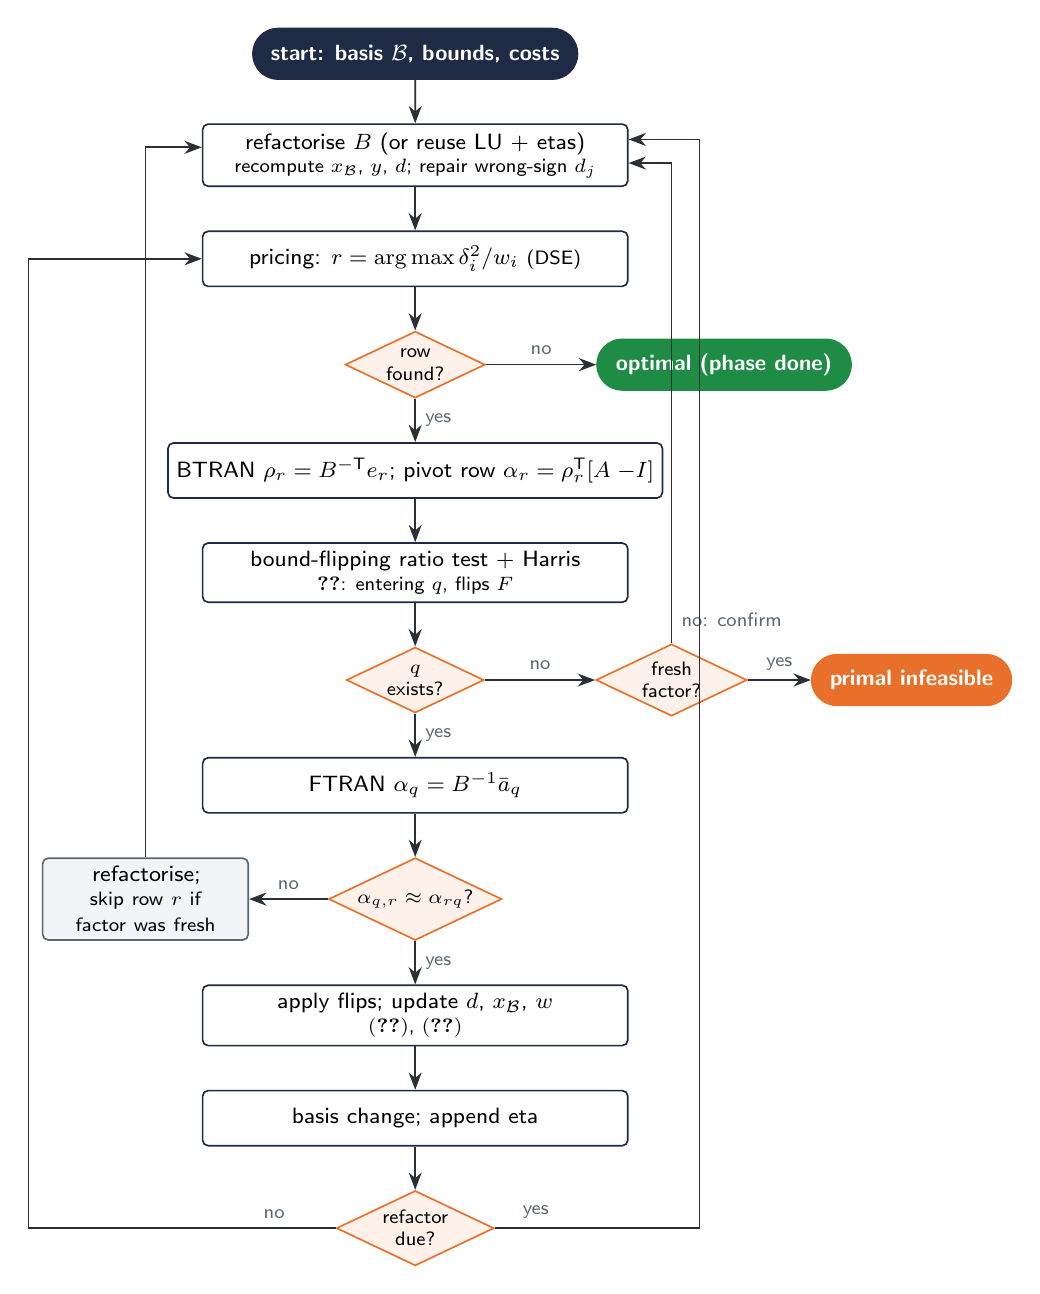
\begin{tikzpicture}[node distance=5.5mm and 8mm]
  \node[term] (start) {start: basis $\mathcal B$, bounds, costs};
  \node[blk,below=of start,minimum width=5.4cm] (fac) {refactorise $B$ (or reuse LU + etas)\\[-1pt]{\scriptsize recompute $x_{\mathcal B}$, $y$, $d$; repair wrong-sign $d_j$}};
  \node[blk,below=of fac,minimum width=5.4cm] (price) {pricing: $r=\arg\max\delta_i^2/w_i$ \scriptsize(DSE)};
  \node[dec,below=of price] (any) {row\\found?};
  \node[term,fill=igreen,draw=igreen,right=14mm of any] (opt) {optimal (phase done)};
  \node[blk,below=of any,minimum width=5.4cm] (row) {BTRAN $\rho_r=B\mT e_r$;\ pivot row $\alpha_r=\rho_r\T[A\;{-I}]$};
  \node[blk,below=of row,minimum width=5.4cm] (ratio) {bound-flipping ratio test + Harris\\[-1pt]{\scriptsize\cref{alg:ratio}: entering $q$, flips $F$}};
  \node[dec,below=of ratio] (cand) {$q$\\exists?};
  \node[dec,right=14mm of cand] (fresh) {fresh\\factor?};
  \node[term,fill=saffron,draw=saffron,right=8mm of fresh] (inf) {primal infeasible};
  \node[blk,below=of cand,minimum width=5.4cm] (ftran) {FTRAN $\alpha_q=B^{-1}\bar a_q$};
  \node[dec,below=of ftran] (agree) {$\alpha_{q,r}\approx\alpha_{rq}$?};
  \node[blkm,left=10mm of agree,text width=2.4cm] (skip) {refactorise;\\[-1pt]{\scriptsize skip row $r$ if factor was fresh}};
  \node[blk,below=of agree,minimum width=5.4cm] (upd) {apply flips; update $d$, $x_{\mathcal B}$, $w$\\[-1pt]{\scriptsize\eqref{eq:updates}, \eqref{eq:dse-update}}};
  \node[blk,below=of upd,minimum width=5.4cm] (chg) {basis change; append eta};
  \node[dec,below=of chg] (due) {refactor\\due?};
  \draw[flow] (start) -- (fac);
  \draw[flow] (fac) -- (price);
  \draw[flow] (price) -- (any);
  \draw[flow] (any) -- node[lbl,above]{no} (opt);
  \draw[flow] (any) -- node[lbl,right]{yes} (row);
  \draw[flow] (row) -- (ratio);
  \draw[flow] (ratio) -- (cand);
  \draw[flow] (cand) -- node[lbl,above]{no} (fresh);
  \draw[flow] (fresh) -- node[lbl,above]{yes} (inf);
  \draw[flow] (fresh.north) -- node[lbl,right,pos=0.3]{no: confirm} ++(0,1.0) |- ([yshift=-1mm]fac.east);
  \draw[flow] (cand) -- node[lbl,right]{yes} (ftran);
  \draw[flow] (ftran) -- (agree);
  \draw[flow] (agree) -- node[lbl,above]{no} (skip);
  \draw[flow] (skip.north) |- ([yshift=1mm]fac.west);
  \draw[flow] (agree) -- node[lbl,right]{yes} (upd);
  \draw[flow] (upd) -- (chg);
  \draw[flow] (chg) -- (due);
  \draw[flow] (due.east) -- node[lbl,above,pos=0.2]{yes} ++(2.6,0) |- ([yshift=2mm]fac.east);
  \draw[flow] (due.west) -- node[lbl,above,pos=0.2]{no} ++(-3.9,0) |- (price.west);
\end{tikzpicture}
\caption[Dual simplex iteration loop]{The dual simplex iteration loop of \file{lp/simplex.py}.
Diamonds are tests. Every path that could declare a result on a possibly inaccurate
factorisation (a missing ratio-test candidate, a pivot that the row and the column see
differently) first refactorises and repeats the iteration.}
\label{fig:simplex-flow}
\end{figure}

\subsection{Phase 1, perturbation and cleanup}
\paragraph{Dual phase 1 by auxiliary boxes}
The all-logical start basis is rarely dual feasible. Following Fourer~\cite{fourer1994}
(Koberstein~\cite[§4.1.2]{koberstein2005}), phase~1 solves the same problem with every bound replaced by
a box:
\begin{equation}\label{eq:aux}
  \text{free}\to[-1,1],\qquad \text{lower only}\to[0,1],\qquad \text{upper only}\to[-1,0],\qquad
  \text{boxed or fixed}\to[0,0].
\end{equation}
Every variable of the auxiliary problem is boxed, so any basis becomes dual feasible once each
nonbasic variable is placed at the bound its reduced cost prefers. The dual simplex therefore starts
at once. An optimal basis of the auxiliary problem is dual feasible for the real problem whenever the
real problem is dual feasible at all. The code does not test the auxiliary objective. Phase~2
starts from the phase-1 basis, and any reduced cost left with the wrong sign is repaired by the
flips and cost shifts described below. If the real problem is dual infeasible (unbounded), the
shifted costs are removed at the end and the primal cleanup finds the unbounded ray.

\paragraph{Cost perturbation}
Degenerate LPs make many ratio-test breakpoints tie at zero, and the dual simplex can then cycle
or stall. Both phases therefore run on perturbed costs~\cite[§6.2.2.3]{koberstein2005}:
\begin{equation}\label{eq:perturb}
  \tilde c_j = c_j + \sigma_j\,5\cdot10^{-7}(1+|c_j|)(1+\xi_j),\qquad \xi_j\sim U[0,1],
\end{equation}
with $\sigma_j=-1$ for a variable at its upper bound and $+1$ otherwise. The direction keeps the
start dual feasible, and the random magnitude breaks the ties. Basic, fixed and free nonbasic
variables are not perturbed. The random factors $\xi$ come from a generator with a fixed seed and are
drawn once per instance, so runs are reproducible and the warm-started re-solves of branch-and-bound
all see the same perturbation.

\paragraph{Cost shifting}
If the entering candidate's reduced cost has the wrong sign (by less than the tolerance, which
the relaxed test allows), its cost is shifted so that $d_q=0$ before the step. The dual objective
then never moves backwards~\cite[§6.2.2.2]{koberstein2005}. After each refactorisation the same fix
is applied to all nonbasics: a boxed variable with a wrong-sign reduced cost is flipped to its other
bound, and any other variable has its cost shifted.

\paragraph{Cleanup by primal simplex}
When phase~2 is optimal, the perturbation and shifts are removed: the true costs are restored and
$y$, $d$ recomputed. Any dual infeasibility that remains is removed by a primal simplex on the same
factorisation. It prices by the largest dual infeasibility, uses a Harris two-pass ratio test over the
basic variables, and flips the entering variable instead of pivoting when it reaches its own
other bound first. The cleanup runs with the dual tolerance tightened to $10^{-9}$
(\cref{sec:simplex-safeguards}). If it loses primal feasibility by more than $10\epsilon_p$, the dual
simplex runs once more. On return the duals are recomputed exactly as $y=B\mT c_{\mathcal B}$ for
the true costs.

\subsection{Warm starts for branch-and-bound}
A \code{SimplexLP} object keeps its factorisation, basis, weights and phase-1 status between calls.
\code{set\_structural\_bounds} changes only the variables whose bounds differ, and re-places
nonbasic ones at their new bounds. \code{get\_basis} and \code{load\_basis} save and restore a basis as
one status byte per variable. If the loaded basis has the same basic set as the current one, the
LU and eta file remain valid and only $x_{\mathcal B}$, $y$ and $d$ are recomputed; otherwise the
basis is refactorised. After a branching change the parent's optimal basis stays dual feasible, so a
child node is typically re-optimised in a few dual pivots.

% Section 7: the LP interior-point method.
\section{The interior-point method for LP}\label{sec:ipm}

\file{lp/ipm.py} implements Mehrotra's predictor--corrector method~\cite{mehrotra1992} on the bounded
standard form \eqref{eq:ipm-form}, with the normal equations solved by the sparse Cholesky of
\cref{sec:chol}. The practical details (free variables, starting point, the normal equations and
their numerical difficulties) follow Wright~\cite[ch.~10--11]{wright1997}. The upper-bound handling
follows Lustig, Marsten and Shanno~\cite{lustig1994}.

\subsection{Newton system}
Write $\mathcal L$ for the variables with a lower bound (after shifting, $x_j\ge0$) and $\mathcal U$
for the boxed ones, and let $X,Z,W,S$ be the diagonal matrices of $x,z,w,s$. The residuals of
\eqref{eq:ipm-kkt} are
\begin{equation}\label{eq:ipm-res}
  r_b = b - Bx,\qquad r_u = U - x - w,\qquad r_c = c - B\T y - z + s,\qquad
  \mu = \frac{x_{\mathcal L}\T z_{\mathcal L} + w\T s}{|\mathcal L|+|\mathcal U|}.
\end{equation}
A Newton step for the perturbed complementarity conditions $XZe=\sigma\mu e$, $WSe=\sigma\mu e$
solves
\begin{equation}\label{eq:newton}
\begin{aligned}
  B\,\Delta x &= r_b, & \Delta x+\Delta w &= r_u, & B\T\Delta y+\Delta z-\Delta s &= r_c,\\
  Z\Delta x + X\Delta z &= r_{xz}, & S\Delta w + W\Delta s &= r_{ws}. &&
\end{aligned}
\end{equation}
Eliminating $\Delta z$, $\Delta w$, $\Delta s$ gives $-\Theta^{-1}\Delta x + B\T\Delta y=\hat r$ with
\begin{equation}\label{eq:theta}
  \Theta^{-1} = X^{-1}Z + W^{-1}S + \Gamma,\qquad
  \hat r = r_c - X^{-1}r_{xz} + W^{-1}(r_{ws}-S r_u),
\end{equation}
where $\Gamma$ is a small primal regularisation: $10^{-8}$ on free variables, which have no barrier
term and would otherwise make $\Theta$ infinite, and $10^{-10}$ elsewhere. Eliminating $\Delta x$
leaves the normal equations
\begin{equation}\label{eq:normal}
  \bigl(B\Theta B\T + \delta I\bigr)\,\Delta y = r_b + B\Theta\hat r,\qquad \delta = 10^{-10},
\end{equation}
and back-substitution recovers
\begin{equation}\label{eq:backsub}
  \Delta x = \Theta(B\T\Delta y-\hat r),\quad
  \Delta z = X^{-1}(r_{xz}-Z\Delta x),\quad
  \Delta w = r_u-\Delta x,\quad
  \Delta s = W^{-1}(r_{ws}-S\Delta w).
\end{equation}
The dual regularisation $\delta$ keeps $M$ positive definite when rows of $B$ are dependent. Each
solve of \eqref{eq:normal} is followed by up to two steps of iterative refinement against the
assembled matrix, $\Delta y\leftarrow\Delta y + M^{-1}(\text{rhs}-M\Delta y)$.

\subsection{Predictor--corrector}
Each iteration factorises $M$ once and solves with it twice:
\begin{enumerate}
  \item \textbf{Predictor} (affine scaling): $r_{xz}=-XZe$, $r_{ws}=-WSe$. The largest steps
        $\alpha_p,\alpha_d\le1$ that keep $x,w$ and $z,s$ nonnegative give the affine
        complementarity $\mu_{\text{aff}}$, and the centring parameter is Mehrotra's
        $\sigma=\min\bigl(1,(\mu_{\text{aff}}/\mu)^3\bigr)$.
  \item \textbf{Corrector:} $r_{xz}=\sigma\mu e - XZe - \Delta X_{\text{aff}}\Delta Z_{\text{aff}}e$,
        and likewise for $(w,s)$. This adds centring and the second-order term the predictor
        neglected.
  \item \textbf{Step:} separate primal and dual step lengths, each the fraction $\eta=0.9995$ of the
        distance to the boundary, capped at~1.
\end{enumerate}

\paragraph{Starting point}
Mehrotra's heuristic, adapted to bounds: with $M_0=BB\T+\delta I$ (factorised once),
$x=B\T M_0^{-1}b$ and $y=M_0^{-1}Bc$. Then $z$ and $s$ are the positive and negative parts of
$c-B\T y$, and $w = U-x$. Each group is shifted to positivity by $1.5$ times its most negative entry,
and all four are then shifted once more by $\frac12 x\T z/\sum z$ and $\frac12 x\T z/\sum x$, which
balances the complementarity products.

\begin{figure}[tbp]
\centering
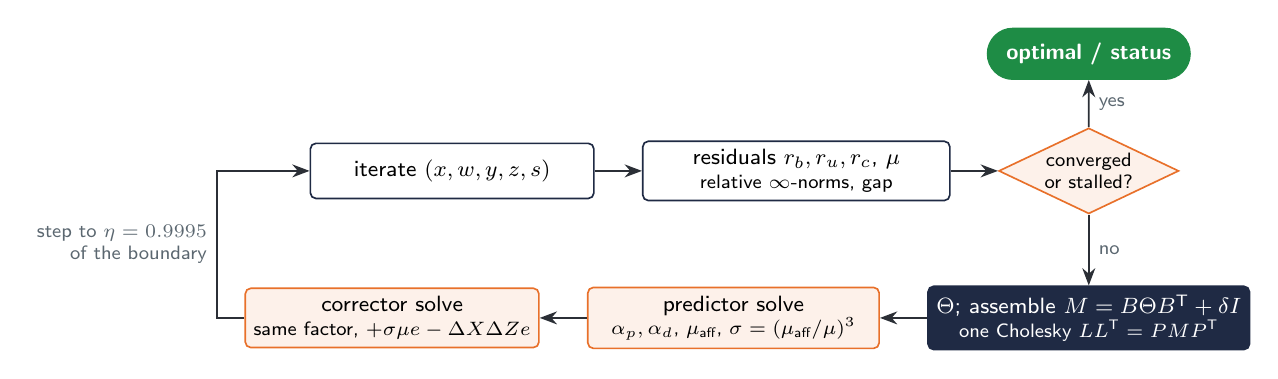
\begin{tikzpicture}[node distance=5mm and 6mm]
  \node[blk,minimum width=3.6cm] (it) {iterate $(x,w,y,z,s)$};
  \node[blk,right=of it,minimum width=3.9cm] (res) {residuals $r_b,r_u,r_c$, $\mu$\\[-1pt]{\scriptsize relative $\infty$-norms, gap}};
  \node[dec,right=of res] (conv) {converged\\or stalled?};
  \node[term,fill=igreen,draw=igreen,above=6mm of conv] (done) {optimal / status};
  \node[blkn,below=9mm of conv,minimum width=3.8cm] (fac) {$\Theta$; assemble $M=B\Theta B\T+\delta I$\\[-1pt]{\scriptsize one Cholesky $LL\T=PMP\T$}};
  \node[blks,left=of fac,minimum width=3.7cm] (pred) {predictor solve\\[-1pt]{\scriptsize$\alpha_p,\alpha_d$, $\mu_{\text{aff}}$, $\sigma=(\mu_{\text{aff}}/\mu)^3$}};
  \node[blks,left=of pred,minimum width=3.4cm] (corr) {corrector solve\\[-1pt]{\scriptsize same factor, $+\sigma\mu e-\Delta X\Delta Ze$}};
  \draw[flow] (it) -- (res);
  \draw[flow] (res) -- (conv);
  \draw[flow] (conv) -- node[lbl,right]{yes} (done);
  \draw[flow] (conv) -- node[lbl,right]{no} (fac);
  \draw[flow] (fac) -- (pred);
  \draw[flow] (pred) -- (corr);
  \draw[flow] (corr.west) -- ++(-0.35,0) |- node[lbl,left,pos=0.25,align=right]{step to $\eta=0.9995$\\of the boundary} (it.west);
\end{tikzpicture}
\caption[Interior-point iteration]{One iteration of the LP interior-point method: one
factorisation of the normal matrix and two solves with it (predictor and corrector). The same loop,
with the augmented system of \cref{fig:kkt} in place of $M$, is the QP method of \cref{sec:qp}.}
\label{fig:ipm}
\end{figure}

\subsection{Termination and stall detection}
Convergence is measured by relative residuals in the $\infty$-norm, the way HiGHS/IPX and most
interior-point codes report them:
\begin{equation}\label{eq:ipm-term}
  p = \frac{\|r_b\|_\infty}{1+\|b\|_\infty}+\frac{\|r_u\|_\infty}{1+\|U\|_\infty},\qquad
  d = \frac{\|r_c\|_\infty}{1+\|c\|_\infty},\qquad
  g = \frac{|c\T x - (b\T y - U\T s)|}{1+|c\T x|},
\end{equation}
and the method stops as \code{optimal} when $p,d,g<10^{-8}$. Near the solution the normal
equations become so ill-conditioned that progress can stop before that point. Continuing then only
drives $\mu$ to zero and $z/x$ to overflow. The method therefore tracks the best error
$e^\star=\min\max(p,d,g)$ so far and counts iterations that fail to halve it:
\begin{itemize}
  \item after 4 such iterations, or once $\mu<10^{-14}(1+|c\T x|)$, the point is accepted as
        \code{optimal} if $p,d,g$ are all below the loose tolerance $10^{-6}$, the accuracy floor
        of the normal equations;
  \item after 30 such iterations it stops with \code{numerical\_error};
  \item a non-finite objective also stops with \code{numerical\_error}.
\end{itemize}
Infeasibility is detected heuristically, from iterates that run off to infinity while the other side
converges: after 20 iterations, $\mu<10^{-12}$, $p>10^{-6}$ and $\|y\|_\infty>10^{12}$ mean primal
infeasible, and $d>10^{-6}$ with $\|x\|_\infty>10^{14}$ means unbounded. A homogeneous self-dual
formulation would give certificates instead, and is on the roadmap.

\begin{algorithm}[t]
\caption{Mehrotra predictor--corrector for LP (\file{lp/ipm.py})}\label{alg:ipm}
\Input{bounded standard form $(B,b,c,U)$, tolerance $\epsilon=10^{-8}$, loose tolerance $10^{-6}$}
analyse the pattern of $BB\T$ once: ordering, elimination tree, slot map\;
starting point (Mehrotra's heuristic); $e^\star\leftarrow\infty$, $k_{\text{stall}}\leftarrow0$\;
\For{$k=1,\dots,200$}{
  compute $r_b,r_u,r_c,\mu$ and $p,d,g$ \eqref{eq:ipm-term}\;
  \lIf{$\max(p,d,g)<\epsilon$}{\Return optimal}
  \leIf{$\max(p,d,g)<e^\star/2$}{$e^\star\leftarrow\max(p,d,g)$, $k_{\text{stall}}\leftarrow0$}{$k_{\text{stall}}\leftarrow k_{\text{stall}}+1$}
  \If{$k_{\text{stall}}\ge4$ or $\mu$ tiny}{
    \lIf{$\max(p,d,g)<10^{-6}$}{\Return optimal}
    \lIf{$k_{\text{stall}}\ge30$}{\Return numerical error}
  }
  infeasibility and unboundedness heuristics\;
  $\Theta\leftarrow(X^{-1}Z+W^{-1}S+\Gamma)^{-1}$; assemble $M$ \eqref{eq:assemble}; factor $LL\T=PMP\T$\;
  predictor: solve \eqref{eq:normal} with $r_{xz}=-XZe$, $r_{ws}=-WSe$; get $\alpha_p,\alpha_d,\mu_{\text{aff}}$\;
  $\sigma\leftarrow\min(1,(\mu_{\text{aff}}/\mu)^3)$\;
  corrector: solve with $r_{xz}=\sigma\mu e-XZe-\Delta X_{\text{aff}}\Delta Z_{\text{aff}}e$ (and $w,s$)\;
  step with $\alpha_p,\alpha_d\leftarrow\min(1,0.9995\,\alpha_{\max})$\;
}
\end{algorithm}

% Section 8: PDLP on CPU and GPU.
\section{PDLP: a first-order LP method on CPU and GPU}\label{sec:pdlp}

The simplex and interior-point methods need sparse factorisations, and those are hard to run
efficiently on a GPU. PDLP~\cite{applegate2021} needs only products with $A$ and $A\T$ and vector
operations, which GPUs do well. \file{lp/pdlp.py} implements the restarted, preconditioned
primal--dual hybrid gradient method (PDHG~\cite{chambolle2011}) with the enhancements of PDLP and of
its GPU descendants cuPDLP.jl~\cite{lu2023cupdlp} and cuPDLP-C~\cite{lu2023cupdlpc}. The method is
written once over an array module (NumPy or CuPy); the inner loop has a Numba backend for the CPU
and a CUDA backend for the GPU.

\subsection{The PDHG step}
For the saddle-point form \eqref{eq:saddle}, one step with primal step $\tau=\eta/\omega$ and dual
step $\sigma=\eta\omega$ (step size $\eta$, primal weight $\omega$) is
\begin{align}
  x' &= \proj_X\bigl(x-\tau(c-A\T y)\bigr),\label{eq:pdhg-x}\\
  y' &= \arg\max_{y\in Y}\; -y\T A(2x'-x) + p(y) - \tfrac{1}{2\sigma}\|y-y_k\|^2 .\label{eq:pdhg-y}
\end{align}
The dual step has a closed form. With $t=y-\sigma A(2x'-x)$, Moreau's identity gives
\begin{equation}\label{eq:moreau}
  y' = t + \sigma\,\proj_{[r^l,r^u]}(-t/\sigma) = t - \clip\bigl(t,\,-\sigma r^u,\,-\sigma r^l\bigr),
\end{equation}
so an equality row gets $y-\sigma(Ax'_{\text{extr}}-b)$, a $\ge$ row gets $\max(0,t+\sigma r^l)$, and a
free row gets~$0$. No slack columns are introduced: ranged rows, bounds and free rows are all
handled by the two projections.

\paragraph{Adaptive steps}
PDLP's step-size rule (its Algorithm~3) accepts a step when $\eta\le\bar\eta$, where
\begin{equation}\label{eq:pdlp-step}
  \bar\eta = \frac{\omega\|x'-x\|^2+\|y'-y\|^2/\omega}{2\,\bigl|(x'-x)\T A\T(y'-y)\bigr|},\qquad
  \eta_{\text{next}} = \min\Bigl(\bigl(1-(k+1)^{-0.3}\bigr)\bar\eta,\ \bigl(1+(k+1)^{-0.6}\bigr)\eta\Bigr).
\end{equation}
A rejected step is not committed and is retried with $\eta_{\text{next}}$. The first step is
$\eta_0=1/\|A\|_{\max}$. Accepted iterates enter a running average weighted by their step size.

\paragraph{Restarts and the primal weight}
Every 64 attempts the method evaluates the primal-weighted KKT error
$\sqrt{\omega\,\|r_p\|^2+\|r_d\|^2/\omega+\text{gap}^2}$ at the current iterate and at the
average, and restarts from the better of the two, following cuPDLP's criteria~\cite{lu2023cupdlp}.
It restarts when that error has fallen below $0.2$ times its value at the last restart; or below $0.8$
times that value while rising since the previous check; or when the iterations since the last restart
exceed $0.36$ of all iterations. Restarts are what give PDHG linear convergence on LPs~\cite{applegate2023}.
At a restart the primal weight is smoothed towards the ratio of dual to primal movement,
\begin{equation}\label{eq:omega}
  \omega \leftarrow \exp\bigl(\theta\log(\|\Delta y\|/\|\Delta x\|)+(1-\theta)\log\omega\bigr),\qquad \theta=0.5 .
\end{equation}

\paragraph{Preconditioning}
Ten Ruiz iterations~\cite{ruiz2001} divide each row and column by the square root of its largest
entry. One Pock--Chambolle pass~\cite{pock2011} ($\alpha=1$) then divides by the square roots of the
row and column $\ell_1$ norms. Finally the bounds and the objective are rescaled by
$\beta_b=1+\|\text{bounds}\|_2$ and $\beta_c=1+\|c\|_2$, as in cuPDLP-C~\cite{lu2023cupdlpc}, so that
$\omega$ starts near~1. The initial weight is $\omega_0=\|c\|/\|b\|$ on the scaled problem.

\paragraph{Termination and infeasibility}
The tests are PDLP's relative ones, evaluated on the \emph{unscaled} problem:
$\|r_p\|_2\le\epsilon(1+\|b\|_2)$, $\|r_d\|_2\le\epsilon(1+\|c\|_2)$ and
$|c\T x-\phi|\le\epsilon(1+|c\T x|+|\phi|)$, where $r_d$ is the part of $c-A\T y$ that the variable
bounds cannot absorb. The default is $\epsilon=10^{-4}$. Every fourth check (256 attempts), the
difference between the current iterate and the one at the previous check is projected onto the
recession cones of the bounds and tested as a Farkas certificate~\cite{applegate2024}. A dual ray
with positive objective and relative infeasibility below $10^{-8}$ proves primal infeasibility; a
primal ray with $c\T\Delta x<0$ proves unboundedness.

The 2-norm primal test alone is not safe. On \code{s250r10} a few right-hand sides are huge
($\|b\|_2\approx2\times10^5$), so the test accepted a point whose worst row was violated by about 20 in
absolute terms: the reported objective was 0.22 away from the optimum, and every bound is finite, so
the dual residual gave no warning. NIRNAY therefore accepts a candidate only if, in addition, every
row satisfies $\mathrm{viol}_i\le10\epsilon\,(1+|b_i|)$ in the original model. A candidate that
fails the row check is counted (\code{row\_check\_rejects}) and the iteration continues. On
\code{s250r10} the GPU run now ends within $3\times10^{-5}$ of the HiGHS objective, at the cost of a
longer run (\cref{tab:large}).

\subsection{Two backends}
\paragraph{CPU}
One Numba call runs a whole block of 64 attempts, in three passes over the data per attempt:
(1)~the primal step \eqref{eq:pdhg-x}; (2)~a row pass that computes $(Ax')_i$ and immediately takes
the dual step \eqref{eq:moreau} for row~$i$; and (3)~a column pass that computes $(A\T y')_j$ together
with the two reductions the step rule \eqref{eq:pdlp-step} needs. The average is updated lazily inside
the next attempt's first two passes. The passes are thread-parallel when $\nnz(A)\ge30\,000$. Below
that, on the development laptop, the fork/join cost of the thread pool outweighed the gain.

\paragraph{GPU}
Each attempt is four CUDA kernels (\cref{fig:gpu}). A \emph{commit} kernel adds the previous accepted
step to the average and takes the primal step. A \emph{rows} kernel computes $Ax'$ with a group of $G$
lanes per row, reducing with warp shuffles, and fuses the dual step. A \emph{columns} kernel computes
$A\T y'$ and fuses $\|\Delta x\|^2$ and $\Delta x\T A\T\Delta y$. A one-thread \emph{step-size}
kernel applies \eqref{eq:pdlp-step}. $G$ is the largest power of two not above the mean row (or
column) length, capped at~32. The accept/reject decision stays on the device: a rejected step is simply
not committed by the next commit kernel. A block of 64 attempts therefore needs no host round trip,
and it is captured once as a CUDA graph and replayed. The host reads one small array of scalars per
check.

\begin{figure}[tbp]
\centering
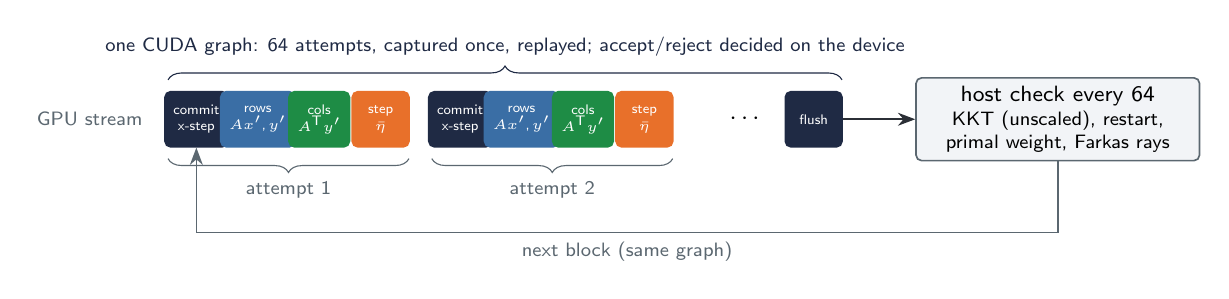
\begin{tikzpicture}[x=1cm,y=1cm]
  \node[lbl,anchor=east] at (-0.2,0) {GPU stream};
  \foreach \a/\x in {1/0,2/3.35} {
    \node[blk,fill=navy,text=white,minimum width=0.72cm,minimum height=0.7cm,font=\sffamily\tiny] (c\a) at (\x+0.36,0) {commit\\x-step};
    \node[blk,fill=sky,draw=sky,text=white,minimum width=0.72cm,minimum height=0.7cm,font=\sffamily\tiny] (r\a) at (\x+1.14,0) {rows\\$Ax'$,\,$y'$};
    \node[blk,fill=igreen,draw=igreen,text=white,minimum width=0.72cm,minimum height=0.7cm,font=\sffamily\tiny] (k\a) at (\x+1.92,0) {cols\\$A\T y'$};
    \node[blk,fill=saffron,draw=saffron,text=white,minimum width=0.72cm,minimum height=0.7cm,font=\sffamily\tiny] (s\a) at (\x+2.7,0) {step\\$\bar\eta$};
  }
  \node[font=\sffamily\small] at (7.35,0) {$\cdots$};
  \node[blk,fill=navy,text=white,minimum width=0.72cm,minimum height=0.7cm,font=\sffamily\tiny] (fl) at (8.2,0) {flush};
  \draw[decorate,decoration={brace,amplitude=5pt,mirror},muted] (0,-0.5) -- node[below=5pt,lbl]{attempt 1} (3.06,-0.5);
  \draw[decorate,decoration={brace,amplitude=5pt,mirror},muted] (3.35,-0.5) -- node[below=5pt,lbl]{attempt 2} (6.41,-0.5);
  \draw[decorate,decoration={brace,amplitude=5pt},navy] (0,0.5) -- node[above=5pt,lbl,text=navy]{one CUDA graph: 64 attempts, captured once, replayed; accept/reject decided on the device} (8.56,0.5);
  \node[blkm,minimum width=3.6cm,align=center] (host) at (11.3,0) {host check every 64\\[-1pt]{\scriptsize KKT (unscaled), restart,}\\[-1pt]{\scriptsize primal weight, Farkas rays}};
  \draw[flow] (fl.east) -- (host.west);
  \draw[flow,muted] (host.south) -- ++(0,-0.9) -| node[lbl,below,pos=0.25]{next block (same graph)} (c1.south);
\end{tikzpicture}
\caption[PDLP on the GPU]{PDLP on the GPU. Each attempt is four fused kernels; the step-size
decision never leaves the device. A block of 64 attempts is one replay of a captured CUDA graph, and
the host is involved only at the check between blocks.}
\label{fig:gpu}
\end{figure}

\subsection{Results}\label{sec:pdlp-results}
\paragraph{Netlib} PDLP at its default tolerance $10^{-4}$ reports \code{optimal} on \nPdlp{} of the
\nPdlpTot{} Netlib problems (\tlPdlp\,s limit). \nPdlpTimeLimit{} hit the time limit
(\pdlpTimeLimitNames) and \nPdlpIterLimit{} the iteration limit (\pdlpIterLimitNames). These are
the badly scaled problems that every PDLP implementation in our comparator study also fails
(\cref{sec:competitors}). A relative KKT tolerance of $10^{-4}$ does not bound the objective error by
$10^{-4}$: \nPdlpTight{} of the problems are within $10^{-4}$ of the HiGHS objective,
\nPdlpLoose{} within $10^{-3}$, and only \nPdlpStrict{} within the $10^{-6}$ used to score the other
engines. The worst objective errors among the ``optimal'' runs are \pdlpWorst. The median run takes
\medItPdlp{} iterations (the longest \maxItPdlp). The shifted geometric mean time is \sgmPdlp\,s
against \sgmPdlpRef\,s for HiGHS. Netlib problems are small and hard, and PDLP is the wrong tool for
them. It is there to show correctness, not speed.

\ifnum\haveLarge=1
\paragraph{Large LPs, CPU against GPU}
The regime PDLP is built for is large, structured LPs. \Cref{tab:large,fig:large} show the
\nLarge{} large instances run so far\ifnum\nLarge<\nLargeList{} (the sweep over \nLargeList{} files is
still running)\fi, from the Mittelmann benchmark sets~\cite{mittelmann}, all at relative tolerance
\largeTol{}, on an \largeGpuHw{} against the CPU backend on the laptop's six cores (12 threads). On
the \nLargeBothOk{} instances both backends finish, the GPU-over-CPU speed-up ranges from
\largeSpeedMin{} to \largeSpeedMax{} (geometric mean \largeSpeedGm; a value below~1 means the GPU was
slower). On \nLargeGpuOnly{} more
(\largeGpuOnlyNames) only the GPU finishes within the \largeLimit\,s limit, and \nLargeNeither{}
finished on neither. HiGHS in the same table runs its interior-point method without crossover at its
default $10^{-8}$ tolerances, which gives the reference objective. That is a far more accurate answer,
so the comparison with the PDLP times is not like for like. HiGHS's interior point at the same
$10^{-4}$ tolerance (last column) is the closer comparison. Where both finish, the ratio of the
high-accuracy HiGHS time to the GPU time ranges from \largeVsHighsMin{} to \largeVsHighsMax.

\begin{table}[ht]
\centering\small
\caption[PDLP on large LPs: CPU against GPU]{PDLP on large LPs (LP relaxations for the MIPLIB
files): wall time of \nirnay{} PDLP on the CPU (Numba, 12 threads) and on the GPU (CuPy), the
relative objective error of the GPU run against the HiGHS reference, and HiGHS's interior point
at its default tolerance (reference) and at the PDLP tolerance. $^\dagger$: stopped at the time
limit; ``$>$'' is then a lower bound on the speed-up. $^\ddagger$: HiGHS did not report
\code{Optimal}.}
\label{tab:large}
\setlength{\tabcolsep}{4pt}
\begin{tabular}{@{}l rrr rrr r rr@{}}
\toprule
 & & & & \multicolumn{3}{c}{\nirnay{} PDLP} & & \multicolumn{2}{c}{HiGHS IPM (s)}\\
\cmidrule(lr){5-7}\cmidrule(l){9-10}
Instance & $m$ & $n$ & nnz & CPU (s) & GPU (s) & $\times$ & rel.\ err & $10^{-8}$ & $10^{-4}$\\
\midrule
\rows{data/large_pdlp.tex}
\bottomrule
\end{tabular}
\end{table}

\begin{figure}[ht]
\centering
\begin{tikzpicture}
\begin{axis}[
  width=0.95\linewidth, height=6cm,
  ybar, bar width=5pt, ymode=log, log origin=infty,
  ylabel={wall time (s)},
  xtick=data, xticklabels from table={data/large_pdlp.dat}{name},
  xticklabel style={font=\ttfamily\scriptsize,rotate=30,anchor=north east},
  enlarge x limits=0.06,
  ymajorgrids, legend style={at={(0.5,1.03)},anchor=south}, legend columns=3,
  ymin=0.1, ymax=1000,
]
\addplot[fill=muted!60,draw=muted] table[x=x,y=cpu] {data/large_pdlp.dat};
\addplot[fill=saffron,draw=saffron] table[x=x,y=gpu] {data/large_pdlp.dat};
\addplot[fill=navy,draw=navy] table[x=x,y=highs] {data/large_pdlp.dat};
\legend{{\nirnay{} PDLP (CPU)},{\nirnay{} PDLP (GPU)},{HiGHS IPM $10^{-8}$}}
\end{axis}
\end{tikzpicture}
\caption[PDLP on large LPs]{Wall time on the large LPs (log scale), from
\file{results/large\_pdlp\_gpu.csv}. The PDLP runs stop at relative tolerance $10^{-4}$;
the HiGHS reference solves to $10^{-8}$.}
\label{fig:large}
\end{figure}
\fi

% Section 9: branch-and-bound for MILP.
\section{Branch-and-bound for mixed-integer programmes}\label{sec:mip}

Every node of the search is the LP relaxation \eqref{eq:simplex-form} with some integer bounds
tightened. A branching change leaves the parent's optimal basis dual feasible, so the dual simplex
re-optimises a child in a few pivots. This is why MILP codes are built on the dual simplex, and
\file{mip/bnb.py} is built on the warm-started \code{SimplexLP} of \cref{sec:simplex}. Its components
follow Achterberg's thesis~\cite{achterberg2007} and the branching study of Achterberg, Koch and
Martin~\cite{achterberg2005}.

\subsection{The search}
\paragraph{Node selection: best bound with plunging}
Open nodes wait in a binary heap keyed by
\begin{equation}\label{eq:heapkey}
  \bigl(\ \underline{z}_{\text{parent}},\ -\text{depth},\ \text{counter}\ \bigr),
\end{equation}
so the node with the smallest bound comes first, and among equal bounds the \emph{deepest}
(\cref{sec:heap}). After a node is branched on, the child that the fractional part favours ($x_j$
rounded up if $f_j\ge0.5$, else down) is solved at once, and the other goes to the heap. The search
keeps diving into the solved child while its bound stays within $10\%$ of the distance between the
best open bound and the cutoff:
\begin{equation}\label{eq:plunge}
  \underline z_{\text{child}} \le \underline z_{\text{open}} + 0.1\,\bigl|z_{\text{cutoff}}-\underline z_{\text{open}}\bigr| .
\end{equation}
Before an incumbent exists the right-hand side is infinite, so the search dives depth-first, which
finds incumbents early. Once one exists it returns to best-first search, which proves the bound.
A child that fails \eqref{eq:plunge} is queued with its own LP bound and basis.

\paragraph{Pruning and bound rounding}
A node is pruned when its LP is infeasible or its rounded bound reaches the cutoff
\begin{equation}\label{eq:cutoff}
  z_{\text{cutoff}} = \begin{cases} z_{\text{inc}} - 1 + 10^{-6} & \text{if the objective is integral on integer points},\\
  z_{\text{inc}} - \max(10^{-9}, 10^{-9}|z_{\text{inc}}|) & \text{otherwise.}\end{cases}
\end{equation}
The objective is integral when every continuous column has zero cost and all costs and $c_0$ are
integers. Node bounds are then rounded up, $\lceil \underline z - 10^{-6}\rceil$, which often closes
the last unit of gap without enumeration. The search stops when the relative gap
$(z_{\text{inc}}-\underline z)/\max(1,|z_{\text{inc}}|)$ is at most $10^{-4}$, the default of HiGHS
and SCIP.

\begin{figure}[tbp]
\centering
\begin{forest}
  for tree={
    draw=navy, rounded corners=2pt, align=center, font=\sffamily\scriptsize,
    inner sep=2pt, minimum width=11mm, l sep=7mm, s sep=9mm, edge={->,draw=ink,line width=0.5pt},
    fill=white,
  }
  [{root\\$\underline z{=}100.3$},fill=navy!12
    [{$x_3\le2$\\$100.6$},edge label={node[midway,left,lbl]{\#1 plunge}},fill=saffron!18,draw=saffron
      [{$x_7\le0$\\$100.8$},edge label={node[midway,left,lbl]{\#2}},fill=saffron!18,draw=saffron
        [{$x_1\le4$\\infeasible},fill=card,draw=muted,edge label={node[midway,left,lbl]{\#3}}]
        [{$x_1\ge5$\\$102$ integral},fill=igreen!12,draw=igreen,edge label={node[midway,right,lbl]{\#4}}]
      ]
      [{$x_7\ge1$\\$100.9$},fill=sky!12,draw=sky,edge label={node[midway,right,lbl]{\#5 from heap}}
        [{$x_2\le1$\\\textbf{101} integral},fill=igreen!25,draw=igreen,edge label={node[midway,left,lbl]{\#6}}]
        [{$x_2\ge2$\\not solved},fill=card,draw=muted,edge label={node[midway,right,lbl]{pruned}}]
      ]
    ]
    [{$x_3\ge3$\\not solved},fill=card,draw=muted,edge label={node[midway,right,lbl]{pruned}}]
  ]
\end{forest}
\caption[Branch-and-bound tree]{An illustrative branch-and-bound tree (made-up numbers, integral
objective). Orange: the plunge, which dives into the favoured child after each branching and finds
the incumbent 102 at node~\#4. The cutoff is then $102-1+10^{-6}$. The open nodes $x_7\ge1$ and
$x_3\ge3$ both have the rounded key $\lceil100.6\rceil=\lceil100.3\rceil=101$; the depth tie-break
of \eqref{eq:heapkey} pops the deeper one (\#5), whose child \#6 is the optimum 101. The new cutoff
$100+10^{-6}$ prunes the two remaining nodes without solving their LPs, and the root bound
$\lceil100.3\rceil=101$ closes the gap.}
\label{fig:bnb}
\end{figure}

\paragraph{Branching: pseudocosts with reliability}
The candidate score is the product rule
\begin{equation}\label{eq:score}
  \text{score}_j = \max\bigl(\psi^-_j f_j,\ 10^{-6}\bigr)\cdot\max\bigl(\psi^+_j(1-f_j),\ 10^{-6}\bigr),
\end{equation}
where $f_j$ is the fractional part of $x_j$ and $\psi^\pm_j$ are the pseudocosts: the average gain in
the LP objective per unit of change, recorded from every solved child. Unobserved directions use the
average over all columns. A candidate is \emph{unreliable} while it has fewer than 4 observations in
either direction. Up to 8 of the best-scored unreliable candidates are then strong-branched, both
children solved by the dual simplex for at most 60 iterations from the current basis, which also
records pseudocosts~\cite{achterberg2005}. If both children are infeasible the node is pruned. If one
is, the candidate gets a top score, because branching on it fixes a variable. An integral child LP
found during strong branching is offered as an incumbent.

\subsection{Domain propagation}\label{sec:propagation}
At every node the bounds are propagated over the rows~\cite{savelsbergh1994,achterberg2007}
(\file{mip/propagate.py}). For a row $r^l\le\sum_j a_jx_j\le r^u$, the minimum and maximum activities
of the row without $x_j$ imply
\begin{equation}\label{eq:propagate}
  a_j>0:\quad x_j\le \frac{r^u-\underline{\text{act}}_{-j}}{a_j},\qquad x_j\ge\frac{r^l-\overline{\text{act}}_{-j}}{a_j},
\end{equation}
with the inequalities reversed for $a_j<0$. Infinite contributions are counted, so a row with exactly
one infinite contributor can still bound that one variable. Integer bounds are rounded inward
($\lfloor u+10^{-6}\rfloor$, $\lceil \ell-10^{-6}\rceil$). A continuous bound is accepted only if it
improves by more than $10^{-3}\max(1,|\text{bound}|)$, so round-off cannot creep into the bounds.
An empty domain, or an activity range that misses the row, proves the node infeasible. Up to 5 passes
run per node. Bounds found for continuous columns guide the search but are not sent to the LP.

\subsection{Primal heuristics}
\begin{itemize}
  \item \textbf{Simple rounding} at every node: round all integer columns of the LP solution and
        accept the point if it is feasible.
  \item \textbf{Fix-and-solve} at the root and every 100 nodes: fix every integer to its rounded
        LP value, propagate, and re-solve the LP for the continuous columns (at most 5\,000
        dual iterations).
  \item \textbf{Fractional diving}~\cite{berthold2006} at the root when no incumbent exists, and every
        50 nodes while none does: repeatedly fix the least fractional integer to its nearest value,
        propagate and re-solve, until the LP is integral, infeasible or worse than the cutoff. The
        LP budget is $\max(1000,\ 2\times$ the LP iterations spent so far$)$.
\end{itemize}

\subsection{Gomory mixed-integer cuts}\label{sec:gmi}
At the root, up to 20 rounds of Gomory mixed-integer (GMI) cuts~\cite{gomory1960,balas1996} tighten
the relaxation (\file{mip/cuts.py}). Take an optimal tableau row whose basic variable is an integer
column with fractional value. Write each nonbasic variable as its distance from the bound it sits
at, $t_k\ge0$, so that $x_B + \sum_k a_k t_k = b$ with $f_0=\fr(b)\in(0,1)$. Every integer-feasible
point then satisfies
\begin{equation}\label{eq:gmi}
  \sum_{\substack{k\ \text{int}\\ f_k\le f_0}}\frac{f_k}{f_0}t_k
  +\sum_{\substack{k\ \text{int}\\ f_k> f_0}}\frac{1-f_k}{1-f_0}t_k
  +\sum_{\substack{k\ \text{cont}\\ a_k>0}}\frac{a_k}{f_0}t_k
  +\sum_{\substack{k\ \text{cont}\\ a_k<0}}\frac{-a_k}{1-f_0}t_k \;\ge\; 1,
  \qquad f_k=\fr(a_k).
\end{equation}
The LP point has $t=0$ and violates the cut by exactly~1. A nonbasic variable counts as integer when its
column is integer and its bound is integral. Logical variables are expanded into the structural
columns of their row, and the cut is mapped back to the unscaled $x$ space.

\paragraph{Numerical safeguards}
Following the practice of Cook, Dash, Fukasawa and Goycoolea~\cite{cook2009}, a cut is generated only
from a row with $0.01<f_0<0.99$. It is skipped when a free nonbasic variable appears in the row or a
needed bound is infinite. Coefficients below $10^{-9}$ of the largest are removed by relaxing against
the variable's bound, which keeps the cut valid. The cut is rejected if its coefficient ratio exceeds
$10^6$ or its efficacy (violation divided by $\|g\|_2$) is below $10^{-5}$, and the survivors are
scaled so that the largest coefficient is~1. A regression test checks that every cut generated on
\code{p0033} keeps the known optimal integer point feasible.

\paragraph{The cut loop}
Each round adds up to $\max(20,\min(200,m/2))$ cuts, most fractional rows first, and re-solves the LP.
The loop stops when the LP is integral, no cut is found, three rounds together move the bound by less
than $0.1\%$, or the cuts have grown the model beyond $4m+1000$ rows. Cuts that are slack at the final
root point are then dropped, because they would only slow down the node LPs.

\begin{algorithm}[t]
\caption{Branch-and-bound with plunging (\file{mip/bnb.py}, simplified)}\label{alg:bnb}
\Input{MILP, gap tolerance $10^{-4}$, time limit}
propagate at the root; solve the root LP; GMI cut rounds; rounding, fix-and-solve, diving\;
$\text{current}\leftarrow$ root (LP solved); heap $\leftarrow\emptyset$\;
\While{time remains}{
  \If{$\text{current}=\emptyset$}{
    pop nodes whose bound $\ge z_{\text{cutoff}}$; \lIf{heap empty}{\textbf{break}}
    pop node with the smallest $(\underline z,-\text{depth})$; propagate; warm-start the dual simplex from its stored basis\;
    record the pseudocost of the branching that created it\;
  }
  \lIf{LP infeasible or $\lceil\underline z\rceil\ge z_{\text{cutoff}}$}{\textbf{continue}}
  \lIf{LP solution integral}{update incumbent; \textbf{continue}}
  simple rounding; periodic diving and fix-and-solve\;
  choose $j$ by reliability branching \eqref{eq:score}\;
  create children $x_j\le\lfloor x_j\rfloor$ and $x_j\ge\lceil x_j\rceil$ with the parent's basis\;
  push the less favoured child; solve the favoured one\;
  \leIf{its bound satisfies \eqref{eq:plunge}}{$\text{current}\leftarrow$ that child}{push it; $\text{current}\leftarrow\emptyset$}
  \lIf{relative gap $\le10^{-4}$}{\textbf{break}}
}
\end{algorithm}

% Section 10: QP interior point.
\section{The interior-point method for convex QP}\label{sec:qp}

With a quadratic objective the normal equations $B(Q+D)^{-1}B\T$ lose their sparsity, because
$(Q+D)^{-1}$ is dense in general. \file{qp/ipm.py} therefore solves the \emph{augmented} system at
every Newton step, factorised by the quasi-definite $LDL\T$ of \cref{sec:ldl}. The outer iteration
is Mehrotra's predictor--corrector, as for LP~\cite{mehrotra1992,wright1997}, in the form Gertz and
Wright give for QP~\cite{gertz2003}. The regularisation follows Friedlander and
Orban~\cite{friedlander2012} and Altman and Gondzio~\cite{altman1999}.

\subsection{The regularised augmented system}
With the bounded standard form \eqref{eq:ipm-form} and $D = X^{-1}Z + W^{-1}S$ (zero on free
variables), the Newton system reduces to
\begin{equation}\label{eq:aug}
  \begin{bmatrix} -(Q+D+\rho I) & B\T\\ B & \delta I\end{bmatrix}
  \begin{bmatrix}\Delta x\\ \Delta y\end{bmatrix} =
  \begin{bmatrix}\hat r\\ r_b\end{bmatrix},\qquad
  \hat r = r_c - X^{-1}r_{xz} + W^{-1}(r_{ws}-Sr_u),
\end{equation}
where now $r_c = c+Qx-B\T y-z+s$. The primal regularisation is $\rho=10^{-10}$ ($10^{-8}$ on free
variables) and the dual regularisation $\delta=10^{-10}$. The matrix is quasi-definite
(\cref{fig:kkt}), so it has an $LDL\T$ factorisation for the minimum-degree order. The pattern of
$K$ is fixed: the triplets of $Q$, the diagonal, $B$ and $B\T$ are sorted once, and each iteration
only sums new values into the fixed slots.

\paragraph{Iterative refinement against the unregularised matrix}
The regularisation perturbs the system being solved. Each solve is therefore followed by up to three
refinement steps in which the residual is computed with the \emph{true} matrix ($\rho=\delta=0$, only
the free-variable term kept) and corrected with the regularised factor:
\begin{equation}\label{eq:refine}
  v \leftarrow v + K_{\text{reg}}^{-1}\bigl(\text{rhs}-K_{\text{true}}\,v\bigr),
\end{equation}
stopping when $\|\text{rhs}-K_{\text{true}}v\|_\infty\le10^{-13}(1+\|\text{rhs}\|_\infty)$. This removes the
effect of $\rho$ and $\delta$ from the direction, while the factorisation keeps the stability they
bring~\cite{friedlander2012}.

\paragraph{Retry with a regularisation boost}
A direction is accepted only if it is finite \emph{and} the refined residual of the augmented system
is below $10^{-6}$ relative to the right-hand side. A factorisation that lost too much to pivot
flooring can return a direction that is finite but wrong: on \code{QRECIPE} it had entries of order
$10^{46}$. If the check fails, the factorisation is repeated with $\rho$ and $\delta$ multiplied by
$10^2$, up to five attempts in all. Only if every attempt fails does the method stop with
\code{numerical\_error}.

\paragraph{Starting point}
The starting point is Mehrotra's heuristic as for LP, with one change. Every component of $x,z,w,s$
is floored at $\max(1,\|b\|_\infty/10^{12})$. When the heuristic lands on a point with tiny
complementarity but large residuals (on \code{YAO}, $\mu\approx2\cdot10^{-6}$ against a dual
infeasibility of $0.5$), the iterates hug the boundary and crawl, and the floor keeps the start well
inside the cone.

\paragraph{Coupled step length}
In LP the primal and dual steps are independent. In QP they are coupled through $Q\Delta x$ in the
dual residual, so with $Q\ne0$ the method takes one common step $\alpha=\min(\alpha_p,\alpha_d)$ by
default, again at the fraction $0.9995$ of the distance to the boundary.

\paragraph{Termination}
The residual measures, the loose-tolerance acceptance on stalling and the infeasibility heuristics are
those of the LP method (\cref{sec:ipm}), with the primal objective $c\T x+\frac12x\T Qx$ and the dual
objective $b\T y-U\T s-\frac12 x\T Qx$ in the gap. The gap is measured relative to
$1+\min(|f|,|f+c_0|)$, that is, also against the objective the user sees, constant included. With a
large constant and an optimum near zero (\code{HS268}, \code{GOULDQP3}), a gap relative to $f$ alone
was far too loose, and points with objective errors near $10^{-5}$ were accepted. Reduced costs are
mapped back as $z=c+Qx-A\T y$ on the original model.

These three changes came from the failure analysis of the first Maros--Mészáros sweep
(\cref{sec:results}). \ifnum\haveQpVone=1 With them, and with the corrected reference of
\cref{sec:verification}, the second sweep solves \nQp{} of \nQpTot{} problems against \nQpVone{} of
\nQpVoneTot{} in the first. The two effects cannot be separated: part of the gain comes from the
reference.\else The sweep that measures their effect is \file{maros\_qpipm\_v2.csv}.\fi

% Section 11: numerical safeguards: what went wrong and how each fix works.
\section{Numerical safeguards: what went wrong and what fixed it}\label{sec:safeguards}

Most of the effort in a simplex or interior-point code goes into its failure modes, not into the
textbook iteration. This section collects the failures we met on the benchmark sets and explains
the mechanism of each fix. The first sweeps (\file{netlib\_simplex\_v1.csv}, \file{netlib\_ipm\_v1.csv})
record the state before the fixes. \Cref{tab:fixes-spx,tab:fixes-ipm} list every problem whose result
changed between versions.

\subsection{Dual simplex}\label{sec:simplex-safeguards}

\begin{table}[tbp]
\centering\small
\caption[Dual simplex: problems changed by the fixes]{Dual simplex, v1 against v2: every Netlib
problem not solved by both versions. v1 solved \nFixedSpxVOne{} of \nFixedSpxVOneTot{}; the fixes of
\cref{sec:simplex-safeguards} solved \nFixedSpx{} more. On the problems both versions finish, v2 is
\nFixedSpxSpeedup{} times faster in shifted geometric mean, measured relative to HiGHS in each sweep.}
\label{tab:fixes-spx}
\begin{tabular}{@{}l lrr lrr@{}}
\toprule
 & \multicolumn{3}{c}{v1} & \multicolumn{3}{c}{v2}\\
\cmidrule(lr){2-4}\cmidrule(l){5-7}
Problem & status & rel.\ err & time (s) & status & rel.\ err & time (s)\\
\midrule
\rows{data/fixes_simplex.tex}
\bottomrule
\end{tabular}
\end{table}

\paragraph{False ``infeasible'' from the ratio test (\code{perold}, \code{pilotnov})}
The v1 sweep declared two feasible problems infeasible within a second. A dual simplex concludes
primal infeasibility when the ratio test finds no entering candidate: the dual is unbounded along the
pivot row, which is a Farkas certificate. That conclusion is only as good as the reduced costs and the
pivot row it rests on. The v1 ratio test did not use the textbook Harris bound. A Harris pass must
bound the step by the \emph{smallest relaxed} ratio $\min_j(|d_j|+\epsilon_d)/|\alpha_{rj}|$ over the
candidates that remain after the bound flips. Only then does a step to any candidate with $t_j\le\Theta$
leave every reduced cost within $\epsilon_d$ of its feasible sign. A step past that bound makes some
$d_j$ infeasible by more than the tolerance. Later ratio tests then exclude that $j$ or treat it
wrongly, and an empty candidate set, and so a false certificate, follows. The fixed kernel
(\cref{alg:ratio}) computes the bound exactly as above. It also makes the pivot tolerance
\emph{relative} to the largest $|\alpha_{rj}|$ in the row, because the \code{pilot} models have rows
whose entries span many orders of magnitude, where an absolute $10^{-7}$ admits pivots that are noise.
Two further guards keep a certificate honest. First, before reporting infeasibility the code
refactorises, recomputes $x_{\mathcal B},y,d$ from scratch, repairs the dual feasibility, and repeats the
iteration; only a second empty ratio test on a fresh factorisation counts. Second, the pivot seen
from the row ($\alpha_{rq}$) and from the column ($\alpha_{q,r}$) must agree to $10^{-6}$ relative, or
the factorisation is renewed.

The source of v1 is not in the repository: the first commit already contains the fixed kernel. This
account is therefore of the fixed code and of the failure recorded in the v1 sweep.

\paragraph{Stalling and cycling in phase 1 (\code{cycle}, \code{pilot87}, \code{tuff})}
Three problems ran into the \tlNetlib\,s limit in v1. Degenerate problems give many zero
reduced costs, so many ratio-test breakpoints tie at zero, and the dual simplex can pivot through a
sequence of degenerate bases without improving the dual objective, possibly returning to a basis
already visited. v1 perturbed the costs in phase~2 only, while phase~1 on Fourer's auxiliary problem
\eqref{eq:aux} is at least as degenerate: every bound there is $0$ or $\pm1$. The fix applies the
random perturbation \eqref{eq:perturb} in phase~1 as well, which breaks the ties. \code{cycle}
went from a time-out to under a second (\cref{tab:fixes-spx}).

\paragraph{Wrong objective on \code{pilot}: the dual tolerance of the cleanup}
v1 returned \code{optimal} on \code{pilot} with a relative objective error far above $10^{-6}$
(\cref{tab:fixes-spx}). The cause is the size of the variable ranges. After the perturbation is removed, reduced costs with the
wrong sign but below the dual tolerance $\epsilon_d=10^{-7}$ are accepted as optimal. The objective
error they leave is bounded by
\begin{equation}\label{eq:dualerr}
  |f(x)-f^\star| \;\lesssim\; \sum_{j\in\mathcal N} |d_j^{\text{infeas}}|\,(u_j-\ell_j),
\end{equation}
and on \code{pilot} a reduced cost of $10^{-8}$ on a variable with a scaled range of $10^3$ already
shifts the objective by $10^{-5}$. The fix polishes with the primal simplex to $\epsilon_d=10^{-9}$ in
the cleanup phase only (phase~1 and phase~2 keep $10^{-7}$, which is enough to steer the search).
v2 solves \code{pilot} to the reference objective (\cref{tab:fixes-spx}).

\paragraph{Singular bases}
Basis repair (\cref{sec:lu}) replaces a dependent basic column by a logical instead of failing; the
number of repairs is reported with each result. Refactorisation every 100 updates, or when the eta
file grows beyond eight times the LU size, bounds the growth of rounding error in the product form.

\paragraph{Exact duals at return}
The iteration updates $d$ incrementally and $y$ only at refactorisation, and cost shifts change $c$
during the loop. The returned $y$ is therefore recomputed as $B\mT c_{\mathcal B}$ for the true costs.
This matters for postsolve (\cref{sec:presolve-bug}) and for anyone who uses the duals as prices, as
refinery planners do.

\subsection{Interior-point method}

\begin{table}[tbp]
\centering\small
\caption[Interior point: problems changed by the fixes]{Interior point, v1 against v2: every Netlib
problem not solved by both versions. v1 solved \nFixedIpmVOne{} of \nFixedIpmVOneTot{}; v2 solves
\nFixedIpm{} more. On problems both versions finish, v2 is \nFixedIpmSpeedup{} times faster in shifted
geometric mean, measured relative to HiGHS in each sweep.}
\label{tab:fixes-ipm}
\begin{tabular}{@{}l lrr lrr@{}}
\toprule
 & \multicolumn{3}{c}{v1} & \multicolumn{3}{c}{v2}\\
\cmidrule(lr){2-4}\cmidrule(l){5-7}
Problem & status & rel.\ err & time (s) & status & rel.\ err & time (s)\\
\midrule
\rows{data/fixes_ipm.tex}
\bottomrule
\end{tabular}
\end{table}

\paragraph{Stall detection}
In v1 several problems (\code{degen3}, \code{greenbeb}, \code{pilot}, \code{pilot87}, \code{dfl001})
ran to the iteration limit, some of them with objectives already correct to $10^{-8}$. Near the
solution $\Theta$ spans many orders of magnitude and the normal equations lose the digits
needed to reach $10^{-8}$. Further iterations only drive $\mu$ towards zero and $z_j/x_j$ towards
overflow. The v2 rule of \cref{sec:ipm} detects this. When the error has not halved in four iterations
(or $\mu$ has collapsed), a point that meets $10^{-6}$ is accepted, and after 30 such iterations the
method gives up with \code{numerical\_error} instead of wandering. Residuals are measured as relative
$\infty$-norms \eqref{eq:ipm-term}, the convention of HiGHS/IPX, so the tolerance means the same on
every problem. The remaining failures (\ipmFailNames) are the problems where even $10^{-6}$ is out of
reach of the normal equations without presolve and crossover (\cref{sec:results}).

\paragraph{Cholesky pivot guard}
Dependent rows make $M$ singular at the limit. A pivot $\le10^{-30}$ is replaced by $10^{128}$
(\cref{sec:chol}), which zeroes that component of $\Delta y$ instead of producing \code{inf}. The dual
regularisation $\delta=10^{-10}$ and the two refinement steps keep the resulting error small. The
numerical errors on \code{grow15} and \code{grow22} in v1 no longer occur.

\subsection{QP interior point: the \texorpdfstring{$LDL\T$}{LDLT} pivot floor}
The augmented matrix is quasi-definite only in exact arithmetic with $\rho,\delta>0$. When $D$
spans many orders of magnitude, cancellation can still produce a pivot of the wrong sign or of
magnitude $10^{-20}$, and dividing by it destroys the factorisation. The kernel replaces any pivot with
$\sigma_kD_{kk}<\delta_{\min}$ by $\sigma_k\delta_{\min}$ (\cref{sec:ldl}), so the inertia is always
right. Without the floor a single bad pivot produces \code{nan} in the direction and ends the solve.
Refinement against the true matrix recovers the accuracy \eqref{eq:refine}. The floor alone is not
enough, though. Flooring many pivots changes the matrix so much that the direction can be finite and
still wrong (\code{QRECIPE}). The method therefore also checks the refined residual of every direction,
and if the check fails it boosts the regularisation by $10^2$ and refactorises (\cref{sec:qp}).

\subsection{Branch-and-bound: heap tie-breaking}\label{sec:heap}
When the objective is integral, node bounds are rounded up, so many open nodes share exactly the
same key. A heap keyed by $(\underline z,\text{counter})$ breaks those ties by insertion order: it
takes the \emph{oldest}, hence shallowest, node among equals. The search then proceeds breadth-first
across a level of equal bounds, the open list grows, and incumbents that a deeper node would give
arrive late. Adding $-\text{depth}$ as the second key \eqref{eq:heapkey} makes ties go to the deepest
node. This changes nothing about which bound is processed next, so the best-bound guarantee is
unchanged. It only makes the search finish subtrees it has already started.

\subsection{Presolve: dual postsolve order}
See \cref{sec:presolve-bug}: singleton-row duals depended on the order in which reductions were
undone, and recording the column's cost and live rows at removal time fixed it.

\begin{lessonbox}[What these failures have in common]
The worst of these bugs produced confident wrong answers (``infeasible'', ``optimal'' with the wrong
objective, duals with the wrong sign) rather than crashes or error messages. Each was found because the benchmark
harness checks every result against an independent solver in a separate process, and because the dual
check tests the optimality conditions on the original model. \Cref{sec:verification} describes these
checks.
\end{lessonbox}

% Section 12: verification methodology.
\section{Verification methodology}\label{sec:verification}

A solver is useful only if its ``optimal'' can be trusted. \nirnay{} is checked at four levels.

\subsection{Independent references, in separate processes}
The harnesses \file{bench/run\_lp.py}, \file{run\_mip.py} and \file{run\_qp.py} run every instance
in a fresh process with a wall-clock limit, so one pathological instance cannot stall or corrupt a
sweep. Each process first solves a tiny instance, so that loading the Numba-compiled code is not
charged to the first real instance, and then times only the solve call (file reading excluded).
The same file is then solved by a reference solver:
\begin{itemize}
  \item \textbf{LP and MILP:} HiGHS~\verHighs~\cite{huangfu2018} with the same time limit, reading its
        own copy of the file;
  \item \textbf{QP:} Clarabel~\verClarabel~\cite{goulart2024}, an interior-point conic solver. HiGHS's
        active-set QP solver times out on the larger Maros--Mészáros problems. The model Clarabel sees
        is read by \emph{HiGHS's} MPS parser, not ours, so a reader bug in \nirnay{} cannot hide by
        affecting both sides. The failure analysis of the first QP sweep found two defects in this
        reference, and the harness was corrected for the second sweep. First, at its default
        tolerances Clarabel's objective is about $10^{-6}$ off on several problems where \nirnay{}
        matches the published optimum, so the reference now runs at $10^{-11}$. Second, a comparison of
        the two parsers (\file{tools/qps\_compare.py}) showed that HiGHS~\verHighs{} misreads the RHS
        section of \code{DPKLO1} and drops coefficients below $10^{-9}$ in \code{HUESTIS},
        \code{HUES-MOD} and \code{KSIP}. On files where the two parsers disagree, the reference now
        solves \nirnay{}'s reading and says so in its status.
\end{itemize}
Neither reference is imported by the \code{nirnay} package. \file{bench/comparators.py}, which drives
the other solvers of \cref{sec:competitors}, carries the same rule in its header.

\subsection{What counts as solved}
With $f$ the objective reported by \nirnay{} and $f^\star$ the reference objective,
\begin{equation}\label{eq:relerr}
  \operatorname{err} = \frac{|f-f^\star|}{\max(1,|f^\star|)} .
\end{equation}
\begin{itemize}
  \item \textbf{LP:} status \code{optimal} and $\operatorname{err}<10^{-6}$;
  \item \textbf{MILP:} status \code{optimal} (relative gap proved $\le10^{-4}$) and
        $\operatorname{err}\le10^{-4}$;
  \item \textbf{QP:} status \code{optimal}, $\operatorname{err}<10^{-6}$, and the reference itself
        reports \code{Solved} or \code{AlmostSolved}. Problems whose reference failed are listed but
        not scored.
\end{itemize}
The harnesses also record the largest row and bound violations (and, for MILP, the integrality
violation) of the returned $x$ on the original model. A wrong answer therefore cannot pass on the
objective alone. PDLP stops at a relative KKT tolerance of $10^{-4}$, and its objective errors are reported
against several thresholds (\cref{sec:pdlp-results}).

\subsection{Optimality conditions after postsolve}
\file{tools/dual\_check.py} tests the conditions \eqref{eq:kkt-lp} directly on the original model: primal
feasibility, and the sign of every $y_i$ and $z_j$ against the activity of its row or bound.
This checks presolve, postsolve, unscaling and the simplex duals together
(\cref{sec:presolve-bug}).
\ifnum\haveDualCheck=1 It currently passes on \nDualOk{} of \nDualTot{} Netlib problems with no
failure; the other \nDualStatus{} stop at its \SI{60}{s} limit.\fi

\subsection{Regression tests and file round trips}
\file{tests/} holds \nTestFunctions{} test functions (many parametrised over several instances). They
check each engine against published optimal values: Koch's final Netlib results~\cite{koch2004}, the
MIPLIB~3 solution values and the Maros--Mészáros repository~\cite{maros1999}. They also check the
kernels (the $LDL\T$ on a random quasi-definite matrix, propagation on a hand-made example), and
that every Gomory cut generated on \code{p0033} keeps the known optimal integer point feasible.
Further tests cover PDLP at three tolerances, on infeasible and unbounded problems, with limits, and
on the GPU. The MPS reader and writer are checked by round trips: read, write and read again gives
identical arrays on the benchmark files, and HiGHS reads the original and the written file into the
same model. The case-study tests re-solve every case file with HiGHS against its stored reference.

\subsection{How speed is measured}
Times are wall-clock seconds on the development laptop (Intel Core i5-11400H, 6 cores / 12 threads,
16\,GB RAM, NVIDIA RTX 3050 Laptop GPU with 4\,GB, Windows~11), taken while other work was running.
Differences below a factor of two on sub-second runs are noise. Two aggregate measures are used:
\begin{itemize}
  \item the \textbf{shifted geometric mean} $\operatorname{sgm}_s(t)=\exp\bigl(\frac1N\sum_i\log(t_i+s)\bigr)-s$,
        with shift $s=\shiftA$\,s (and $s=\shiftB$\,s as a check). The shift keeps sub-millisecond
        instances from dominating a ratio of means. It also compresses ratios on small instances,
        so we additionally report the plain geometric mean and the median of per-instance time ratios;
  \item \textbf{performance profiles}~\cite{dolan2002}: for solver $s$ on problem $p$ let
        $r_{p,s}=t_{p,s}/\min_{s'}t_{p,s'}$ ($\infty$ if $s$ failed). The profile
        $\rho_s(\tau)=\frac1N|\{p: r_{p,s}\le\tau\}|$ is the fraction of problems $s$ solves within a
        factor $\tau$ of the fastest. $\rho_s(1)$ is how often $s$ is fastest, and $\rho_s(\infty)$ how
        often it solves at all.
\end{itemize}

% Section 13: benchmark results and failure analysis.
\section{Benchmark results}\label{sec:results}

\pgfplotsset{discard if not/.style 2 args={
  x filter/.append code={\edef\tempa{\thisrow{#1}}\edef\tempb{#2}\ifx\tempa\tempb\else\def\pgfmathresult{inf}\fi}}}

Three public test sets are used, all with published optimal values: the \nSpxTot{} LPs of
Netlib~\cite{gay1985}, from $\netlibMinRows$ to $\netlibMaxRows$ rows and up to \netlibMaxNnz{}
nonzeros (\code{\netlibMaxName}); the \nMipList{} MILPs of MIPLIB~3~\cite{bixby1998}; and the
\nQpList{} convex QPs of Maros and Mészáros~\cite{maros1999}. The large LPs of \cref{sec:pdlp} come
from Mittelmann's benchmark sets~\cite{mittelmann}. Every number below is read from the result files
named in the captions. \Cref{tab:summary} gives the overview and \cref{fig:bars} the solved counts.

\ifnum\haveInProgress=1
\begin{keybox}[Sweeps still running when this report was built]
\file{gen\_data.py} analyses the newest sweep of each suite that covers every instance. The following
newer sweeps were still running and are not yet in the headline numbers: \inProgressList. Where a
comparison with them is meaningful on the instances finished so far, the text gives it and says so.
Rerunning \file{gen\_data.py} and \code{latexmk} after they finish updates every number.
\end{keybox}
\fi

\begin{table}[tbp]
\centering\small
\caption[Summary of the benchmark sweeps]{Summary of the benchmark sweeps. ``Solved'' uses the
criteria of \cref{sec:verification}. Times are shifted geometric means (shift \shiftA\,s) over the
instances \nirnay{} solves, for \nirnay{} and for the reference on the same instances.}
\label{tab:summary}
\begin{tabular}{@{}l l l r r r r@{}}
\toprule
Suite & Engine & Reference & Solved & \nirnay{} (s) & Ref.\ (s) & Ratio\\
\midrule
Netlib LP & dual simplex (\spxVer) & HiGHS & \nSpx/\nSpxTot & \sgmSpx & \sgmSpxRef & \ratioSpx\\
Netlib LP & interior point (\ipmVer) & HiGHS & \nIpm/\nIpmTot & \sgmIpm & \sgmIpmRef & \ratioIpm\\
Netlib LP & PDLP, $10^{-4}$ & HiGHS & \nPdlp/\nPdlpTot$^{a}$ & \sgmPdlp & \sgmPdlpRef & \ratioPdlp\\
MIPLIB 3 & branch-and-bound (\mipVer) & HiGHS & \nMip/\nMipTot$^{b}$ & \sgmMip & \sgmMipRef & \ratioMip\\
Maros--Mészáros & QP interior point & Clarabel & \nQp/\nQpTot & \sgmQp & \sgmQpRef & \ratioQp\\
\bottomrule
\multicolumn{7}{@{}l}{\footnotesize $^a$ status \code{optimal} at relative KKT $10^{-4}$; objective errors in \cref{sec:pdlp-results}.\quad
$^b$ \tlMip\,s limit; HiGHS proves \nMipRefOpt.}
\end{tabular}
\end{table}

\begin{figure}[tbp]
\centering
\begin{tikzpicture}
\begin{axis}[
  width=0.82\linewidth, height=5.2cm,
  xbar, bar shift=0pt, bar width=9pt,
  xmin=0, enlarge y limits=0.14,
  ytick=data, yticklabels from table={data/solved_bars.dat}{label},
  y dir=reverse,
  xlabel={instances},
  xmajorgrids,
  nodes near coords, nodes near coords style={font=\sffamily\scriptsize},
  every node near coord/.append style={anchor=west},
  legend style={at={(1,1.03)},anchor=south east}, legend columns=2,
]
\addplot[fill=rule,draw=muted] table[x=total,y=x] {data/solved_bars.dat};
\addplot[fill=saffron,draw=saffron!80!black,nodes near coords style={text=white,anchor=east}] table[x=solved,y=x] {data/solved_bars.dat};
\legend{instances run, solved}
\end{axis}
\end{tikzpicture}
\caption[Solved instances per suite]{Solved instances per suite and engine (from
\file{data/solved\_bars.dat}, generated from \file{results/}). PDLP counts status \code{optimal} at its
$10^{-4}$ tolerance.}
\label{fig:bars}
\end{figure}

\subsection{Netlib LP: correctness}
The dual simplex solves all \nSpx{} of the \nSpxTot{} Netlib problems to the reference objective
(file \file{\spxFile}). The median relative objective error is \medErrSpx{} and the largest \maxErrSpx{},
so the answers are vertex solutions exact to rounding. The interior-point method solves \nIpm{} (median
error \medErrIpm, largest \maxErrIpm). \Cref{fig:ecdf} shows the distribution of the errors for every
engine. The interior-point failures are analysed in \cref{sec:ipm-fail}.

\begin{figure}[tbp]
\centering
\begin{tikzpicture}
\begin{axis}[
  width=0.9\linewidth, height=6cm,
  xlabel={$\log_{10}$ relative objective error against the reference},
  ylabel={fraction of scored instances},
  xmin=-17.2, xmax=0, ymin=0, ymax=1.02,
  grid=major, legend cell align=left,
  legend style={at={(0.5,-0.22)},anchor=north}, legend columns=2,
]
\addplot[nspx,const plot] table[x=logerr,y=frac] {data/ecdf_spx.dat};
\addplot[nipm,const plot] table[x=logerr,y=frac] {data/ecdf_ipm.dat};
\addplot[npdlp,const plot] table[x=logerr,y=frac] {data/ecdf_pdlp.dat};
\addplot[igreen,line width=1.1pt,const plot] table[x=logerr,y=frac] {data/ecdf_qp.dat};
\addplot[navy,line width=1.1pt,densely dashed,const plot] table[x=logerr,y=frac] {data/ecdf_mip.dat};
\addplot[muted,dashed,forget plot] coordinates {(-6,0) (-6,1.02)};
\addplot[muted,dashed,forget plot] coordinates {(-4,0) (-4,1.02)};
\legend{dual simplex (Netlib), interior point (Netlib), {PDLP, status optimal (Netlib)}, QP interior point (Maros--Mészáros), branch-and-bound (MIPLIB 3)}
\end{axis}
\end{tikzpicture}
\caption[Distribution of relative objective errors]{Cumulative distribution of the relative
objective error \eqref{eq:relerr} over the instances each engine reports optimal (for LP, QP and the
dual simplex: the instances counted as solved; for PDLP: every status \code{optimal}). Errors of
exactly zero are plotted at $10^{-17}$. Dashed lines: the $10^{-6}$ LP/QP and $10^{-4}$ MILP criteria.}
\label{fig:ecdf}
\end{figure}

\subsection{Netlib LP: speed}
\Cref{fig:profile} shows the performance profiles of the dual simplex, the interior-point method and
HiGHS on Netlib, and \cref{fig:scatter} plots every instance's time against the reference's.

\begin{honestbox}[Speed, stated plainly]
\nirnay{}'s dual simplex is faster than HiGHS on \nFasterSpx{} of the \nSpx{} Netlib problems it solves.
Its shifted geometric mean time is \sgmSpx\,s against \sgmSpxRef\,s, a ratio of \ratioSpx{} with a
\shiftA\,s shift and \ratioSpxTenShift{} with a \shiftB\,s shift. The per-instance ratios have
geometric mean \gmrSpx{}, median \medrSpx{} and maximum \maxrSpx{}. The shifted mean understates the
gap because most Netlib problems solve in milliseconds, so the per-instance ratios are the fairer
summary: \nirnay{} is about \gmrSpx{} times slower. On load-normalised times (\cref{fig:profile}), the
interior-point method is faster than the simplex on \nIpmFasterThanSpx{} of the \nBothSolved{} problems
both solve, and taking the faster of the two engines on each problem gives a shifted-mean ratio of
\bestOfTwoRatio{} against HiGHS.
\end{honestbox}

\begin{figure}[tbp]
\centering
\begin{tikzpicture}
\begin{axis}[
  width=0.9\linewidth, height=6.2cm,
  xmode=log, log basis x=2,
  xmin=1, xmax=\profTauMax, ymin=0, ymax=1.02,
  xlabel={$\tau$ (time relative to the fastest of the solvers shown)},
  ylabel={$\rho_s(\tau)$},
  grid=major, legend pos=south east, legend cell align=left,
  log number format basis/.code 2 args={\pgfmathparse{#1^#2}\pgfmathprintnumber{\pgfmathresult}},
]
\addplot[nhighs,const plot] table[x=tau,y=rho] {data/profile_highs.dat};
\addplot[nspx,const plot] table[x=tau,y=rho] {data/profile_spx.dat};
\addplot[nipm,const plot] table[x=tau,y=rho] {data/profile_ipm.dat};
\legend{HiGHS, \nirnay{} dual simplex, \nirnay{} interior point}
\end{axis}
\end{tikzpicture}
\caption[Performance profile on Netlib]{Dolan--Moré performance profile on the \nProf{} Netlib
problems. Times come from \file{\spxFile} and \file{\ipmFile}. The two sweeps ran under different
machine load (HiGHS itself was \sweepLoadRatio{} times slower, in geometric mean, in the first than in
the second), so each engine's time is rescaled by the ratio of the common HiGHS time (the geometric
mean of its two measurements) to HiGHS's time in that engine's sweep. HiGHS is
fastest on a fraction \rhoOneHighs{} of the problems. The dual simplex is within a factor of 10 of the
fastest on a fraction \rhoTenSpx{} and within \tauAllSpx{} on all of them. The interior-point
method's curve stays below~1 because of its failures.}
\label{fig:profile}
\end{figure}

\begin{figure}[tbp]
\centering
\begin{tikzpicture}
\begin{groupplot}[
  group style={group size=2 by 2, horizontal sep=14mm, vertical sep=16mm},
  width=0.49\linewidth, height=0.47\linewidth,
  xmode=log, ymode=log,
  xlabel={reference time (s)}, ylabel={\nirnay{} time (s)},
  grid=major, unbounded coords=discard,
  title style={font=\sffamily\footnotesize\bfseries,color=navy},
]
\nextgroupplot[title={Netlib: dual simplex vs.\ HiGHS}, xmin=1e-4, xmax=1e3, ymin=1e-4, ymax=1e3]
  \addplot[muted,dashed,domain=1e-4:1e3,samples=2,forget plot] {x};
  \addplot[muted!60,dotted,domain=1e-4:1e2,samples=2,forget plot] {10*x};
  \addplot[only marks,mark=*,mark size=1.3pt,color=saffron,discard if not={ok}{1}] table[x=ref,y=time] {data/scatter_spx.dat};
  \addplot[only marks,mark=x,mark size=2.4pt,color=navy,thick,discard if not={ok}{0}] table[x=ref,y=time] {data/scatter_spx.dat};
\nextgroupplot[title={Netlib: interior point vs.\ HiGHS}, xmin=1e-4, xmax=1e3, ymin=1e-4, ymax=1e3]
  \addplot[muted,dashed,domain=1e-4:1e3,samples=2,forget plot] {x};
  \addplot[muted!60,dotted,domain=1e-4:1e2,samples=2,forget plot] {10*x};
  \addplot[only marks,mark=*,mark size=1.3pt,color=sky,discard if not={ok}{1}] table[x=ref,y=time] {data/scatter_ipm.dat};
  \addplot[only marks,mark=x,mark size=2.4pt,color=navy,thick,discard if not={ok}{0}] table[x=ref,y=time] {data/scatter_ipm.dat};
\nextgroupplot[title={MIPLIB 3: branch-and-bound vs.\ HiGHS}, xmin=1e-2, xmax=2e2, ymin=1e-2, ymax=2e2]
  \addplot[muted,dashed,domain=1e-2:2e2,samples=2,forget plot] {x};
  \addplot[muted!60,dotted,domain=1e-2:2e1,samples=2,forget plot] {10*x};
  \addplot[only marks,mark=*,mark size=1.3pt,color=igreen,discard if not={ok}{1}] table[x=ref,y=time] {data/scatter_mip.dat};
  \addplot[only marks,mark=x,mark size=2.4pt,color=navy,thick,discard if not={ok}{0}] table[x=ref,y=time] {data/scatter_mip.dat};
\nextgroupplot[title={Maros--Mészáros: QP-IPM vs.\ Clarabel}, xmin=1e-4, xmax=1e3, ymin=1e-4, ymax=1e3]
  \addplot[muted,dashed,domain=1e-4:1e3,samples=2,forget plot] {x};
  \addplot[muted!60,dotted,domain=1e-4:1e2,samples=2,forget plot] {10*x};
  \addplot[only marks,mark=*,mark size=1.3pt,color=plum,discard if not={ok}{1}] table[x=ref,y=time] {data/scatter_qp.dat};
  \addplot[only marks,mark=x,mark size=2.4pt,color=navy,thick,discard if not={ok}{0}] table[x=ref,y=time] {data/scatter_qp.dat};
\end{groupplot}
\end{tikzpicture}
\caption[Time against reference time]{Time of \nirnay{} against the time of the reference solver, per
instance, on log--log axes. Dots: solved; crosses: not solved (plotted at the time used). Dashed:
equal time; dotted: ten times slower. Points above the dashed line are instances where \nirnay{} is
slower. On MIPLIB the \tlMip\,s limit shows as a horizontal row of crosses.}
\label{fig:scatter}
\end{figure}

\paragraph{Where the time goes}
The iteration counts are reasonable: the median Netlib solve takes \medItSpx{} dual iterations, and
\cref{fig:iters} shows the count growing roughly in proportion to $m+n$, as expected for a dual simplex.
The cost is in each iteration. Every step calls several compiled kernels (pricing, BTRAN, pivot row,
ratio test, two or three FTRANs, updates) from a Python loop. On small problems the Python overhead
of each call exceeds the arithmetic. On large ones the linear algebra is less refined than in
production codes: FTRAN and BTRAN work on dense vectors of length $m$ instead of exploiting
hyper-sparsity, the product-form update grows the eta file where a Forrest--Tomlin update would
modify $U$ in place. \ifnum\spxHasPresolve=1 The simplex sweep analysed here runs with presolve,
which is still written in plain Python; its cost and benefit are measured in \cref{sec:presolve}.\else
The sweeps analysed here ran without presolve; its effect is measured in \cref{sec:presolve}.\fi{} \Cref{sec:roadmap} lists the remedies in the order we expect them to pay.

\begin{figure}[tbp]
\centering
\begin{tikzpicture}
\begin{axis}[
  width=0.62\linewidth, height=5.2cm, xmode=log, ymode=log,
  xlabel={$m+n$ (rows + columns)}, ylabel={dual simplex iterations},
  grid=major, legend pos=north west, legend cell align=left,
]
\addplot[only marks,mark=*,mark size=1.2pt,color=saffron] table[x=mn,y=iters] {data/iters_spx.dat};
\addplot[muted,dashed,domain=40:30000,samples=2] {x};
\legend{Netlib problems, iterations $=m+n$}
\end{axis}
\end{tikzpicture}
\caption[Dual simplex iterations against problem size]{Dual simplex iterations (phase~1, phase~2
and cleanup together) against $m+n$ on the Netlib problems.}
\label{fig:iters}
\end{figure}

\subsection{Interior-point failures}\label{sec:ipm-fail}
\begin{table}[ht]
\centering\small
\caption[Interior-point failures on Netlib]{Netlib problems the interior-point method does not solve (\file{\ipmFile}).}
\label{tab:ipm-fail}
\begin{tabular}{@{}l rr l r r r@{}}
\toprule
Problem & $m$ & $n$ & status & rel.\ err & time (s) & iterations\\
\midrule
\rows{data/ipm_failures.tex}
\bottomrule
\end{tabular}
\end{table}
\Cref{tab:ipm-fail} lists the failures. All end in the stall rule's
\code{numerical\_error}, and \nIpmNear{} of them are within $10^{-3}$ of the optimum when they stop. These
are the problems known to be hard for interior-point methods without presolve. The comparator study
found Clarabel and GLPK's interior point also failing on \code{greenbea} without presolve. The
\code{pilot} models have coefficients spanning many orders of magnitude, and \code{dfl001}'s normal
matrix fills heavily. Production IPMs solve them with presolve, crossover to a basis, and
more careful handling of free variables. Within \nirnay{}, the dual simplex solves all of them.

\subsection{MIPLIB 3}\label{sec:mip-results}
\ifnum\nMipTot<\nMipList
\begin{keybox}[Partial sweep]
The MIPLIB sweep (\file{\mipFile}) had finished \nMipTot{} of the \nMipList{} instances when this
report was built. The numbers below cover those instances and update when \file{gen\_data.py} is rerun.
\end{keybox}
\fi
With a \tlMip\,s limit, branch-and-bound proves \nMip{} of \nMipTot{} instances optimal, all with the
reference objective. No instance was declared optimal with a wrong objective (\nMipWrongOpt{}). HiGHS,
under the same limit, proves \nMipRefOpt. \nMipBothOpt{} instances are proved by both, \nMipRefOnly{}
only by HiGHS, and \nMipOnlyUs{} only by \nirnay{}. \nirnay{} is faster than HiGHS on \nFasterMip{}
of its solved instances (\fasterMipNames). On the instances it solves, its shifted geometric mean time is
\sgmMip\,s against \sgmMipRef\,s for HiGHS, \ratioMip{} times slower.

The instances not proved fall into three groups:
\begin{itemize}
  \item \textbf{optimum found, not proved} (\nMipFoundNotProved): \mipFoundNotProvedNames. The incumbent is
        optimal, but the bound does not close in time;
  \item \textbf{incumbent with a gap} (\nMipIncumbent{} with an incumbent at the limit, of which
        \nMipGapBelowOnePct{} are within $1\%$ and \nMipGapBelowTenPct{} within $10\%$), see \cref{fig:gaps};
  \item \textbf{no incumbent at all} (\nMipNoIncumbent): \mipNoIncumbentNames. These are mostly
        large set-partitioning and network-design models, where rounding and diving fail and each LP is
        expensive.
\end{itemize}
The causes are the ones the comparator study (\cref{sec:competitors}) points to. \nirnay{}'s MIP presolve
only tightens bounds. Its only cut family is Gomory mixed-integer; production codes add MIR, knapsack
cover, flow cover, clique and zero-half cuts. It has no feasibility pump, no feasibility jump and no
large-neighbourhood search. Node throughput is low: the median solved instance processes
\mipNodesPerSec{} nodes per second at a median of \mipLpItersPerNode{} dual iterations per node, and
each node pays the Python overhead of the simplex driver. The largest search on record took
\maxNodesMip{} nodes.

\begin{figure}[tbp]
\centering
\begin{tikzpicture}
\begin{axis}[
  width=0.8\linewidth, y=10.5pt,
  xbar, bar width=6pt, xmode=log, log origin=infty,
  xmin=1e-4, xmax=2,
  ytick=data, yticklabels from table={data/mip_gaps.dat}{name},
  yticklabel style={font=\ttfamily\scriptsize},
  xlabel={relative gap at the time limit}, xmajorgrids, enlarge y limits={abs=0.7},
  y dir=reverse,
]
\addplot[fill=saffron,draw=saffron!80!black] table[x=gap,y=idx] {data/mip_gaps.dat};
\end{axis}
\end{tikzpicture}
\caption[MIPLIB 3: gap at the time limit]{MIPLIB~3 instances that reached the \tlMip\,s limit with an
incumbent: relative gap $|f-\underline z|/\max(1,|f|)$ at the limit (log scale). The target is $10^{-4}$.}
\label{fig:gaps}
\end{figure}

\ifnum\haveMipVtwo=1
\paragraph{Effect of cuts and presolve} The sweep with Gomory cuts and presolve
(\file{\mipNewerFile})\ifnum\mipNewerPartial=1{} was still running when this report was built, with
\mipNewerDone{} of \nMiplibFiles{} instances finished\fi. It proves \mipNewerSolved{} of them optimal.
On the \nMipCommon{} instances both sweeps cover, it proves \nMipCutsGained{} instances that v1 (no
cuts, no presolve) did not (\mipGainedNames), and loses \nMipCutsLost{} (\mipLostNames).
\fi

\subsection{Maros--Mészáros QP}
The QP interior point solves \nQp{} of the \nQpTot{} problems (\file{\qpFile}), with a median error of
\medErrQp{} and a median of \medItQp{} iterations (the most \maxItQp). It is faster than Clarabel on
\nFasterQp{} of them, and slower by a factor of \ratioQp{} in shifted geometric mean. The rest divide as
follows:
\begin{itemize}
  \item \textbf{reference failed} (\nQpRefBad): \qpRefBadNames. Clarabel did not report a solution,
        so these count as not solved whatever \nirnay{} returned;
  \item \textbf{accepted loosely} (\nQpLoose): \qpLooseNames. \nirnay{} reports \code{optimal} with an
        objective error between $10^{-6}$ and $10^{-3}$ against the reference: points whose relative
        residuals met the tolerance while the objective error did not (or, see below, reference error);
  \item \textbf{wrong answer} (\nQpWrongBig): \qpWrongBigNames. Reported \code{optimal} with a large
        objective error against the reference;
  \item \textbf{numerical error} (\nQpNumErr): \qpNumErrNames. The stall rule gave up. Clarabel itself
        reports only \code{AlmostSolved} on \nQpAlmostRef{} of the problems \nirnay{} does not solve;
  \item \textbf{other} (\nQpOther): \qpOtherNames. The solve stopped at the time limit, or the
        benchmark process returned no status; these count as not solved.
\end{itemize}
\ifnum\nQpLooseOrWrong>0 The wrong and loose answers show the weak point of the QP method: its
termination rule trusts relative residuals that do not bound the objective error on badly scaled
problems.\else No problem is reported \code{optimal} with an objective error above $10^{-6}$: every
failure is an honest status (numerical error, time limit) rather than a wrong answer.\fi{}
\ifnum\nQpRefAnnotated>0 On \nQpRefAnnotated{} files the two MPS parsers disagree, and the reference
solves \nirnay{}'s reading (\cref{sec:verification}).\fi{}
\ifnum\qpVerNum=1 Not every entry above is \nirnay{}'s fault. This sweep used the first version of the
QP reference, whose two defects are described in \cref{sec:verification}: Clarabel at default
tolerances, and HiGHS's parser misreading \code{DPKLO1} and dropping small coefficients in
\code{HUESTIS}, \code{HUES-MOD} and \code{KSIP}. Some ``loose'' and ``wrong'' entries, \code{DPKLO1} among
them, may be reference errors, and the corrected reference will tell. The changes described in \cref{sec:qp} (the gap measured with the objective
constant, the residual check on every direction, and the floored starting point) were made in response
to this sweep. \ifnum\haveQpNew=1 The sweep that measures them was still running when this report was
built.\fi\fi{} Presolve is not yet applied to QPs. \Cref{tab:maros-full} in the appendix lists every
problem.

% Section 14: industrial case studies.
\section{Industrial case studies}\label{sec:cases}

Benchmarks show that a solver is correct; case studies show that it fits the problems the problem
statement is about. \file{nirnay/cases/} builds \nCases{} optimisation models from public data, most of
it Indian. Every module carries a \code{CASE\_INFO} record of its sources (URL and licence), of what is
taken from them unchanged, and of what is assumed. \file{docs/CASE\_STUDIES.md} documents each model in
full. Each case is written to \file{data/cases/<case>.mps} and re-solved by HiGHS as a reference.
\Cref{tab:cases} gives the sizes.

\begin{table}[ht]
\centering\small
\caption[Case-study models]{Case-study models: problem class and size of the default instance, read
from the MPS files in \file{data/cases/} (integer columns in parentheses).}
\label{tab:cases}
\begin{tabularx}{\linewidth}{@{}X l l r r r@{}}
\toprule
Case & Module & Class & Rows & Columns & Nonzeros\\
\midrule
\rows{data/cases_sizes.tex}
\bottomrule
\end{tabularx}
\end{table}

\subsection{The models}
\paragraph{Refinery crude selection and blending (LP)}
The model chooses how much of each crude to run on each of MRPL's three crude distillation units
(capacities from MRPL's public project filing), where each distillation cut goes, and how to blend
BS-VI petrol (MS\,91, MS\,95), BS-VI diesel, ATF, LPG, naphtha and fuel oil to the BIS
specifications (IS~2796, IS~1460, IS~1571), to maximise gross margin at PPAC's 2024--25 average
prices. Crude assays come from the US Department of Energy's Strategic Petroleum Reserve (public
domain). Every cut of every crude is its own stream, so the property blending is linear. For a product
pool $P$ with components $i$ of mass $m_i$ and density $\rho_i$, a volumetric specification such as the
octane number is written
\begin{equation}\label{eq:blend}
  \sum_{i\in P}\frac{m_i}{\rho_i}\bigl(\mathrm{RON}_i-\mathrm{RON}_{\min}\bigr)\ \ge\ 0 ,
\end{equation}
which is linear in the mass flows. Density, cetane index, smoke point, naphthalenes and sulphur are
handled the same way.

\paragraph{Twelve-month production plan (MILP)}
Twelve monthly copies of the refinery network are linked by product inventories and storage limits.
Crude is bought in integer parcels, at most three crudes are processed per month (tank segregation),
and the FCC severity is a binary choice with at most two changeovers per year. Monthly demand follows
PPAC's national consumption pattern.

\paragraph{Thermal unit commitment (MILP)}
The 73 thermal units of the RTS-GMLC system over 48 hours, with the tight and compact formulation of
Morales-España, Latorre and Ramos~\cite{moralesespana2013} as published with PGLib-UC: on, start and
stop binaries, start-up categories, ramping, minimum up and down times, spinning reserve, and a
piecewise-linear production cost.

\paragraph{Economic dispatch with a DC network (QP)}
Quadratic generation cost over the 2000-bus PGLib-OPF case, with DC power flow, line limits and
angle-difference limits. The HiGHS optimum matches the DC objective PGLib-OPF publishes for the case.

\paragraph{Capacitated facility location (MILP)}
OR-Library's \code{capb} instance~\cite{beasley1990} (100 depots, 1000 customers) with the strong
linking constraints $x_{ij}\le y_i$. The HiGHS optimum equals the published optimum. It stands in for
depot and terminal network design, for which no Indian dataset with costs and capacities is public.

\paragraph{BS-VI fuel distribution across India (LP)}
A transport model from 21 Indian refineries to 36 states and union territories. It meets every state's
2024--25 MS and HSD sales (PPAC) with the least tonne-kilometres, using refinery and state locations
from Wikidata.

\paragraph{Crude-oil unloading and blending schedule (MILP)}
The crude scheduling problems of Lee et al.~\cite{lee1996} in the multi-operation sequencing
formulation of Mouret, Grossmann and Pestiaux~\cite{mouret2009} (the MILP relaxation that is the first
step of their method). All four instances reproduce the published optimal values.

\subsection{Reference solutions and \nirnay{}'s results}
\Cref{tab:cases-ref} gives the HiGHS reference for each case file, and \cref{tab:cases-runs} the
record of \nirnay{}'s runs kept in the case-study document.

\begin{table}[ht]
\centering\small
\caption[HiGHS reference results for the cases]{HiGHS \verHighs{} reference results for the case files
(\file{data/cases/reference.csv}). Refinery objectives are negative gross margins in thousand US\$.
The unit-commitment reference was solved to a \ucGapTarget\% gap target (final gap \ucGap\%), as in
PGLib-UC's own reference script, so it is not a proven optimum.}
\label{tab:cases-ref}
\begin{tabular}{@{}l l l r r r@{}}
\toprule
Case & Class & Status & Objective & MIP gap & Time (s)\\
\midrule
\rows{data/cases_ref.tex}
\bottomrule
\end{tabular}
\end{table}

\ifnum\haveCaseRuns=1
\begin{table}[ht]
\centering\small
\caption[\nirnay{} on the case studies]{\nirnay{} on the case studies (from the ``NIRNAY on the
cases'' record in \file{docs/CASE\_STUDIES.md}; one process per run, 120\,s limit, times including
Numba compilation on first call).}
\label{tab:cases-runs}
\begin{tabular}{@{}l l l r r r@{}}
\toprule
Case & Method & Status & Objective & Rel.\ diff. & Time (s)\\
\midrule
\rows{data/cases_runs.tex}
\bottomrule
\end{tabular}
\end{table}

\nCaseRunsOptimal{} of the \nCaseRuns{} recorded runs reach the HiGHS optimum: both LP cases with the
simplex and the interior point, and the economic dispatch QP. The MILP cases do not yet solve.
The twelve-month refinery plan stops at the time limit with a poor incumbent, the crude schedule
returns nothing within the wall limit, and unit commitment and facility location, the two largest
models in \cref{tab:cases}, were not attempted with branch-and-bound. This is the same gap as on MIPLIB
(\cref{sec:mip-results}), and closing it is the first item of the roadmap.
\fi

% Section 15: competitor analysis summary.
\section{Competitor analysis}\label{sec:competitors}

Before deciding what to build next, we installed and ran the established solvers on the development
machine and read their logs (\file{docs/COMPETITOR\_ANALYSIS.md}, driver \file{bench/comparators.py}).
The field covers HiGHS (dual simplex, IPX interior point, two PDLP variants, MIP, QP), SCIP with SoPlex,
Google OR-Tools (GLOP, PDLP, CLP, CBC, SCIP, CP-SAT), CBC, GLPK, Clarabel, OSQP and NVIDIA cuOpt on the
GPU. CPLEX, Gurobi and Xpress are commercial and were not installed. Each (instance, solver) pair ran in
its own process at default settings on small sets of \nCompLpInst{} Netlib LPs, \nCompMipInst{} MIPLIB~3
instances and \nCompQpInst{} Maros--Mészáros QPs. \Cref{tab:comp-lp,tab:comp-mip,tab:comp-qp} add
\nirnay{}'s own results on the same instances, taken from its sweeps.

\begin{table}[ht]
\centering\small
\caption[Comparator solvers on the Netlib LP set]{Comparator solvers on the LP set (\CompLpInstances).
Solved: objective within $10^{-6}$ of the reference ($10^{-3}$ for the first-order PDLP and OSQP runs,
whose default tolerances are loose). Times: shifted geometric mean over the solved instances and the
largest time. From \file{results/comparators\_lp.csv} and \nirnay{}'s sweeps; sorted by solved count,
then time.}
\label{tab:comp-lp}
\begin{tabular}{@{}l l r r r@{}}
\toprule
Solver & Platform & Solved & sgm (s) & max (s)\\
\midrule
\rows{data/comp_complp.tex}
\bottomrule
\end{tabular}
\end{table}

\begin{table}[ht]
\centering\small
\begin{minipage}[t]{0.52\linewidth}
\centering\footnotesize\setlength{\tabcolsep}{3pt}
\captionof{table}[Comparator solvers on the MIPLIB 3 set]{MIP set (\CompMipInstances); solved: optimal within $10^{-4}$. $^\ast$: GPU.}
\label{tab:comp-mip}
\begin{tabular}{@{}l r r r@{}}
\toprule
Solver & Solved & sgm (s) & max (s)\\
\midrule
\rows{data/comp_compmip_short.tex}
\bottomrule
\end{tabular}
\end{minipage}\hfill
\begin{minipage}[t]{0.45\linewidth}
\centering\footnotesize\setlength{\tabcolsep}{3pt}
\captionof{table}[Comparator solvers on the Maros--Mészáros set]{QP set (\CompQpInstances); solved: within $10^{-6}$ ($10^{-3}$ for OSQP).}
\label{tab:comp-qp}
\begin{tabular}{@{}l r r r@{}}
\toprule
Solver & Solved & sgm (s) & max (s)\\
\midrule
\rows{data/comp_compqp_short.tex}
\bottomrule
\end{tabular}
\end{minipage}
\end{table}

\subsection{What the comparison shows}
\begin{itemize}
  \item \textbf{Every winner is a dual simplex first.} HiGHS, SoPlex inside SCIP, GLOP and cuOpt's
        concurrent mode all rely on a dual simplex for small and medium LPs and for node LPs. The
        interior point is the alternative for large LPs, and PDLP a third engine for very large LPs at
        low accuracy. cuOpt races all three and takes the first answer, and on the small Netlib LPs its
        own concurrent mode always picked the CPU dual simplex. \nirnay{} has the same three engines;
        running them concurrently is on the roadmap.
  \item \textbf{PDLP failures are algorithmic.} Every PDLP implementation tested failed on the same
        badly scaled Netlib problems (\code{pilot4}, \code{greenbea}), as ours does. On large,
        structured LPs the picture reverses: GPU PDLP beats every factorisation-based method on the
        laptop (\cref{sec:pdlp-results}).
  \item \textbf{Presolve matters more than anything else.} A census of HiGHS's presolve on Netlib and
        MIPLIB~3 shows that singleton rows, doubleton equations, the aggregator (free-column
        substitution), forcing rows, and fixed and dominated columns do most of the work. It is also what
        makes an interior point robust: Clarabel and GLPK's interior point fail on \code{greenbea}
        without it, and HiGHS's IPX succeeds with it.
  \item \textbf{MIP gaps close at the root.} Gomory mixed-integer and (c-)MIR cuts are the common core
        of SCIP, CBC and cuOpt, with knapsack cover, zero-half, clique and implied-bound cuts next. First
        incumbents come from cheap heuristics run before or right after the first LP (HiGHS's
        feasibility jump, SCIP's trivial, locks and shifting heuristics).
  \item \textbf{References make mistakes too.} The study found a wrong ``optimal'' from one solver's
        MIP on \code{p0201}, a ``Solved'' status at a $10^{-3}$ objective error from another on
        \code{greenbea}, false infeasibility verdicts from GLPK's interior point, and a time-limit
        defect in one PDLP. \nirnay{}'s harness therefore scores against a reference in a separate
        process and records the reference's own status (\cref{sec:verification}).
\end{itemize}

\subsection{Licences and cost}
All the open-source comparators are free: HiGHS (MIT), SCIP and OR-Tools, Clarabel, OSQP and cuOpt
(Apache-2.0), CBC (EPL-2.0), and GLPK (GPL-3.0, whose copyleft prevents linking into a non-GPL product).
CPLEX, Gurobi and Xpress are proprietary: their free editions are limited in model size, and
production licences are sold per user or per deployment, with prices quoted on request. \nirnay{} is
intended to be released under Apache-2.0, like most of the open-source field, and because it depends
on no solver library, no licence restriction flows into it.

% Section 16: limitations and roadmap.
\section{Limitations and roadmap}\label{sec:roadmap}

\subsection{Limitations}
\begin{itemize}
  \item \textbf{Speed.} The dual simplex is about \gmrSpx{} times slower than HiGHS on Netlib
        (geometric mean of per-instance ratios; \ratioSpx{} in shifted geometric mean), and
        branch-and-bound is \ratioMip{} times slower on the MIPLIB instances it solves. The iteration
        drivers are Python; only the kernels are compiled.
  \item \textbf{MILP strength.} \nMip{} of \nMipTot{} MIPLIB~3 instances are proved optimal in
        \tlMip\,s against \nMipRefOpt{} for HiGHS. The MILP case studies do not yet solve. MIP presolve
        only tightens bounds, Gomory mixed-integer is the only cut family, the heuristics are simple, and
        there is no parallel tree search.
  \item \textbf{Presolve.} Only reductions with a simple exact postsolve exist so far
        (\cref{sec:presolve}). Doubleton equations, forcing rows, dominated columns, parallel rows and
        columns, and coefficient tightening are missing, and QPs are not presolved at all.
  \item \textbf{Interior points.} Infeasibility is detected heuristically, not certified. There is no
        crossover to a basic solution, and the QP termination test can accept a point whose
        objective is wrong (\cref{sec:results}).
  \item \textbf{Linear algebra.} FTRAN and BTRAN use dense work vectors, updates are product-form, and
        the Cholesky is up-looking rather than supernodal, so it uses no dense BLAS kernels.
  \item \textbf{Scope.} No MIQP, no second-order cones, no SOS constraints, no callbacks or modelling
        layer beyond the Python API and MPS files.
\end{itemize}

\subsection{Roadmap, in order of expected payoff}
\begin{enumerate}
  \item \textbf{Move the simplex driver into compiled code.} Moving the whole iteration into one Numba
        (or C) loop removes the per-call overhead that dominates small problems. We expect this to be
        the largest single speed-up.
  \item \textbf{Complete presolve}, following the census order: doubleton equations and the
        aggregator, forcing rows, dominated columns, parallel rows and columns, then MIP coefficient
        tightening and probing.
  \item \textbf{MIP:} MIR and knapsack-cover cuts with a cut pool and ageing, feasibility jump and a
        feasibility pump for first incumbents, RINS/RENS-style neighbourhood search, reduced-cost fixing
        and a root restart.
  \item \textbf{Linear algebra:} hyper-sparse FTRAN/BTRAN, a Forrest--Tomlin update, and a supernodal
        Cholesky/$LDL\T$ with dense kernels, which would also make a GPU factorisation possible.
  \item \textbf{Interior points:} a homogeneous self-dual formulation for certified infeasibility,
        crossover to a vertex, and a stricter QP gap test.
  \item \textbf{Concurrent LP:} race dual simplex, interior point and GPU PDLP and take the first answer,
        as cuOpt does. The three engines already exist.
  \item \textbf{Refinery-scale validation:} run the case-study MILPs to proven optimality, and add
        MRPL's own planning models when they become available.
\end{enumerate}

\subsection{Conclusion}
\nirnay{} shows that a solver meeting the independence requirement of SIH26119 can be built: every
factorisation and algorithm is our own, the answers are verified against independent solvers, and on
the standard LP and QP test sets it is correct. It is not yet fast, and its MILP code is far behind the
state of the art. The report documents both the engine and its numerical failures, so the work can be
continued.


\clearpage
\phantomsection
\addcontentsline{toc}{section}{References}
\bibliographystyle{plainnat}
\bibliography{refs}

\clearpage
\appendix
% Appendices: full result tables, typesetting toolchain, reproduction.
\section{Full benchmark tables}\label{app:tables}

$^\dagger$ marks a result that does not count as solved under the criteria of \cref{sec:verification}.
Times are in seconds, and ``rel.\ err'' is the relative objective error \eqref{eq:relerr}.

{\small
\setlength{\tabcolsep}{4pt}
\begin{longtable}{@{}l rrr r rr rr rr@{}}
\caption[Netlib: every problem, all three LP engines]{Netlib: every problem, with the dual simplex
(\file{\spxFile}), the interior point (\file{\ipmFile}) and PDLP at $10^{-4}$ (\file{\pdlpFile}; for
PDLP $^\dagger$ marks an objective error of $10^{-3}$ or more).}\label{tab:netlib-full}\\
\toprule
 & & & & HiGHS & \multicolumn{2}{c}{dual simplex} & \multicolumn{2}{c}{interior point} & \multicolumn{2}{c}{PDLP}\\
\cmidrule(lr){6-7}\cmidrule(lr){8-9}\cmidrule(l){10-11}
Problem & $m$ & $n$ & nnz & time & time & rel.\ err & time & rel.\ err & time & rel.\ err\\
\midrule
\endfirsthead
\toprule
Problem & $m$ & $n$ & nnz & HiGHS & time & rel.\ err & time & rel.\ err & time & rel.\ err\\
\midrule
\endhead
\bottomrule
\endfoot
\rows{data/netlib_full.tex}
\end{longtable}
}

{\small
\setlength{\tabcolsep}{4pt}
\begin{longtable}{@{}l rrr l r r r rr l@{}}
\caption[MIPLIB 3: every instance run]{MIPLIB~3: every instance run so far (\file{\mipFile},
\tlMip\,s limit). ``ref'' is HiGHS's outcome under the same limit (opt: proved optimal; TL: time
limit).}\label{tab:miplib-full}\\
\toprule
Instance & $m$ & $n$ & int & status & gap & rel.\ err & nodes & time & HiGHS & ref\\
\midrule
\endfirsthead
\toprule
Instance & $m$ & $n$ & int & status & gap & rel.\ err & nodes & time & HiGHS & ref\\
\midrule
\endhead
\bottomrule
\endfoot
\rows{data/miplib_full.tex}
\end{longtable}
}

{\small
\setlength{\tabcolsep}{4pt}
\begin{longtable}{@{}l rrr l l r r rr@{}}
\caption[Maros--Mészáros: every problem]{Maros--Mészáros convex QPs: every problem (\file{\qpFile}).
``Clarabel'' is the reference's own status; $^{\S}$: the MPS parsers disagree on this file and the
reference solves \nirnay{}'s reading (\cref{sec:verification}).}\label{tab:maros-full}\\
\toprule
Problem & $m$ & $n$ & nnz & status & Clarabel & rel.\ err & iters & time & ref.\ time\\
\midrule
\endfirsthead
\toprule
Problem & $m$ & $n$ & nnz & status & Clarabel & rel.\ err & iters & time & ref.\ time\\
\midrule
\endhead
\bottomrule
\endfoot
\rows{data/maros_full.tex}
\end{longtable}
}

\section{Typesetting toolchain}\label{app:toolchain}
The report is built with pdf\LaTeX{} from TeX Live 2023 by \code{latexmk}. Every figure is drawn in
TikZ or PGFPlots from source, with no raster images, and every plot and generated table reads files
that \file{gen\_data.py} writes from \file{results/*.csv}. The packages were chosen after checking their
CTAN pages for maintenance status and licence, and for how widely they are used on
TeX~StackExchange, where \code{tikz-pgf} and \code{pgfplots} are among the most-used tags.

\begin{center}\small
\begin{tabularx}{\linewidth}{@{}l X@{}}
\toprule
Package & Why it was chosen\\
\midrule
TikZ/PGF 3.1 & The standard native drawing system for \LaTeX{} (actively maintained, LPPL/GPL). Used
  with the libraries \code{positioning}, \code{arrows.meta}, \code{shapes.geometric},
  \code{shapes.misc}, \code{fit}, \code{calc}, \code{backgrounds}, \code{matrix} and
  \code{decorations.pathreplacing} for the architecture, data-flow, flowchart, KKT and fill-in
  figures. \url{https://ctan.org/pkg/pgf}\\
PGFPlots 1.18 & Plots computed by \TeX{} from data files, in the document's fonts; log axes,
  \code{groupplots} for the scatter panel, \code{const plot} for profiles and ECDFs.
  \url{https://ctan.org/pkg/pgfplots}\\
pgfplotstable & Reads CSV/whitespace tables directly (tick labels read from the \code{.dat}
  files). \url{https://ctan.org/pkg/pgfplotstable}\\
forest & Trees from a bracket notation with automatic, compact packing; used for the
  branch-and-bound tree. \url{https://ctan.org/pkg/forest}\\
algorithm2e & Floating pseudocode with numbered lines and block rules, referenced with
  \code{cleveref}. It was preferred to \code{algorithmicx}, whose CTAN entry lists its maintainer as
  inactive. \url{https://ctan.org/pkg/algorithm2e}\\
booktabs, longtable, tabularx & Professional table rules; multi-page appendix tables.
  \url{https://ctan.org/pkg/booktabs}\\
siunitx & Consistent typesetting of the generated numbers (\code{\textbackslash num\{1.7e-16\}}).
  \url{https://ctan.org/pkg/siunitx}\\
tcolorbox & The summary, lesson and ``honest'' boxes. \url{https://ctan.org/pkg/tcolorbox}\\
listings & Code listings. \url{https://ctan.org/pkg/listings}\\
hyperref, cleveref & Links and automatic reference names (``Figure'', ``Algorithm'').
  \url{https://ctan.org/pkg/cleveref}\\
microtype & Character protrusion and font expansion for even text colour.
  \url{https://ctan.org/pkg/microtype}\\
natbib + \code{plainnat} & Numbered citations with DOIs. \code{biblatex}/\code{biber} would be the
  modern choice, but the TeX Live installation on the build machine does not include
  \code{biblatex}, and natbib builds everywhere. \url{https://ctan.org/pkg/natbib}\\
libertinus, Source Sans/Code Pro & Open fonts with matching mathematics (Libertinus) and a
  sans-serif for headings and figures. \url{https://ctan.org/pkg/libertinus}\\
\bottomrule
\end{tabularx}
\end{center}
\code{tikz-cd} was considered and not used: none of the diagrams is a commutative diagram.

\section{Reproducing this report}\label{app:repro}
\begin{lstlisting}[language=bash]
# benchmark sweeps (each writes results/<suite>.csv)
python bench/run_lp.py  data/netlib --method simplex --limit 300 --out results/netlib_simplex_v3.csv
python bench/run_lp.py  data/netlib --method ipm     --limit 300 --out results/netlib_ipm_v2.csv
python bench/run_mip.py data/miplib --limit 60 --out results/miplib3_bnb_v2.csv
python bench/run_qp.py  data/qp/mm  --limit 120 --out results/maros_qpipm_v1.csv
python bench/run_pdlp_gpu.py data/large --tol 1e-4 --limit 300 --out results/large_pdlp_gpu.csv
python tools/dual_check.py data/netlib/*.mps.gz > deliverables/report/data/dual_check.txt

# data for the report (picks the newest version of every sweep), then the PDF
cd deliverables/report
python gen_data.py
latexmk -pdf -interaction=nonstopmode main.tex
\end{lstlisting}
\file{gen\_data.py} prefers the highest \code{\_v<k>} version of each sweep, so a new sweep appears in
the report as soon as its file exists. It was last run on \genDate.


\end{document}
